% !TEX root = main.tex


% 文章的主体架构章节数均在此设计编辑。


\documentclass[UTF8,twoside,zihao=-4,AutoFakeBold,scheme=chinese,openany]{ctexbook}
\usepackage{graphicx}
% 输入配置文件,例如调用的宏包(公式,插图等)

%设置文章格式

\usepackage[final]{pdfpages}

\usepackage{geometry}
\usepackage{makecell}
\usepackage{caption}
\usepackage{multirow}
\usepackage{booktabs}
\makeatletter
\let\c@lofdepth\relax
\let\c@lotdepth\relax
\makeatother
\usepackage{subfigure}
\usepackage{float}
\usepackage[titles,subfigure]{tocloft}
\usepackage{soul}
\usepackage{color,xcolor}
\usepackage{setspace}
\usepackage{titletoc}
\usepackage{longtable}

\usepackage[list=off]{bicaption}
\usepackage[hidelinks]{hyperref}
%\usepackage{mathptmx} %设置数学公式为新罗马字体
\usepackage{amsmath} %几个数学宏包
\usepackage{fontspec}
%\usepackage{mathspec}
%\usepackage[no-math]{fontspec}
\usepackage{newtxmath}
\usepackage{bm}
%\usepackage{newtxtext}
%\usepackage{unicode-math}
%\usepackage{txfonts}
\usepackage{diagbox}
\usepackage{tabularray}
\UseTblrLibrary{diagbox}

\AtBeginDocument{\DeclareMathAlphabet{\mathbf}{OT1}{cmr}{bx}{n}}







% 设置页边距
\geometry{a4paper,top=3cm,bottom=3cm,left=3cm,right=3cm}

% 设置行间距 1.5倍
%\linespread{1.4}\selectfont

% 设置段与段之间的垂直距离 \parskip默认橡皮长度是0pt plus 1pt
\setlength{\parskip}{0pt}
%\setlength{\baselineskip}{20pt}
% \setlength{\parindent}{0pt}
%\setlength{\intextsep}{6pt}         % 调整正文中浮动体与文字之间的距离

% 行间距={}*字体里面的第二个{},对于xiaosi而言就是1等于20磅
\linespread{1}\selectfont

%设置字体
% 设置英文字体
\setmainfont{Times New Roman}[
BoldFont = Times New Roman Bold,
ItalicFont = Times New Roman Italic,
BoldItalicFont = Times New Roman Bold Italic
]

\setsansfont{Times New Roman}[
BoldFont = Times New Roman Bold,
ItalicFont = Times New Roman Italic,
BoldItalicFont = Times New Roman Bold Italic
]

\setmonofont{Times New Roman}[
BoldFont = Times New Roman Bold,
ItalicFont = Times New Roman Italic,
BoldItalicFont = Times New Roman Bold Italic
]

%设置字号,举例\xiaosi表示的是20磅行距,\xiaosid对应的是单倍行距


\usepackage{ctexsize,type1cm}
\newcommand{\chuhaod}{\fontsize{42pt}{54.6pt}\selectfont}
\newcommand{\xiaochud}{\fontsize{36pt}{46.8pt}\selectfont}
%\newcommand{\yihao}{\fontsize{26pt}{39pt}\selectfont}
%\newcommand{\xiaoyi}{\fontsize{24pt}{36pt}\selectfont}   
\newcommand{\erhaod}{\fontsize{22pt}{28.6pt}\selectfont}          
\newcommand{\xiaoerd}{\fontsize{18pt}{23.4pt}\selectfont}          
\newcommand{\sanhaod}{\fontsize{16pt}{20.8pt}\selectfont}        
\newcommand{\xiaosand}{\fontsize{15pt}{19.5pt}\selectfont}        
\newcommand{\sihaod}{\fontsize{14pt}{18.2pt}\selectfont}            
\newcommand{\xiaosid}{\fontsize{12pt}{15.6pt}\selectfont}            
\newcommand{\wuhaod}{\fontsize{10.5pt}{13.65pt}\selectfont}
%\newcommand{\xiaowu}{\fontsize{9pt}{13.5pt}\selectfont}    
%\newcommand{\liuhao}{\fontsize{7.5pt}{11.25pt}\selectfont}

\newcommand{\wuhaob}{\fontsize{10.5pt}{17pt}\selectfont}

\newcommand{\chuhao}{\fontsize{42pt}{42pt}\selectfont}
\newcommand{\xiaochu}{\fontsize{36pt}{36pt}\selectfont}
\newcommand{\yihao}{\fontsize{26pt}{39pt}\selectfont}
\newcommand{\xiaoyi}{\fontsize{24pt}{36pt}\selectfont}   
%\newcommand{\erhao}{\fontsize{22pt}{33pt}\selectfont}          
\newcommand{\xiaoer}{\fontsize{18pt}{27pt}\selectfont}          
\newcommand{\sanhao}{\fontsize{16pt}{20pt}\selectfont}        
\newcommand{\xiaosan}{\fontsize{15pt}{20pt}\selectfont}        
\newcommand{\sihao}{\fontsize{14pt}{20pt}\selectfont}            
\newcommand{\xiaosi}{\fontsize{12pt}{20pt}\selectfont}            
\newcommand{\wuhao}{\fontsize{10.5pt}{20pt}\selectfont}
\newcommand{\xiaowu}{\fontsize{9pt}{13.5pt}\selectfont}    
\newcommand{\liuhao}{\fontsize{7.5pt}{11.25pt}\selectfont}

%使用公式,表格,图片
% 先取消原先的 \Bbbk 宏的定义,避免与后续宏包加载产生冲突。
\let\Bbbk\relax
\usepackage{mathtools,amsmath,amssymb,graphicx,array,float,bbm}

%按照章节编号
\numberwithin{figure}{chapter}
\numberwithin{table}{chapter}
\numberwithin{equation}{chapter}

%图、表、公式格式改为 X-X
\renewcommand\thefigure{\arabic{chapter}-\arabic{figure}}
\captionsetup[figure]{labelsep=space}

\renewcommand\thetable{\arabic{chapter}-\arabic{table}}
\captionsetup[table]{labelsep=space}

\renewcommand\theequation{\arabic{chapter}-\arabic{equation}}

%设置图表英文标题格式
\captionsetup{font={stretch=1.2}} %调整中英文图表标题的行距
\setlength{\abovecaptionskip}{6pt} %调整图表标题与图片和表格之间的距离
%\setlength{\belowcaptionskip}{1pt} 
\captionsetup[figure][bi-second]{name=\wuhao Fig.}
\captionsetup[table][bi-second]{name=\wuhao Table}
%\setlength{\captionwidth}{10cm} 




% 设置页眉面脚
%% 设置章节前的页码格式
%\usepackage[pagestyles]{titlesec}
%\newpagestyle{MyStyle}{
	%  \setfoot{}{\Roman{page}}{}
	%%  \headrule
	%}

\usepackage{fancyhdr}

%\fancypagestyle{abstract}
%{
	%	\fancyhf{}
	%	\renewcommand{\headrulewidth}{0.5pt}
	%	%	\renewcommand{\footrulewidth}{0mm}
	%	\fancyfoot[C]{\songti\xiaowu \Roman{page}}
	%	\fancyhead[C]{\wuhao \leftmark}
	%}

%重新设置plain,chapter设置页眉时会调用plain,因此需要重新定义plain,不能设置为其他名称



\fancypagestyle{plain}{
	\fancyhf{}
	\fancyfoot[C]{\songti\xiaowu  \Roman{page} }
	\fancyhead[C]{\songti\wuhao \leftmark}
}





%页眉设置,博士和硕士学位论文请在下面自行修改
\fancypagestyle{body}{
	\fancyhf{}
	\fancyfoot[C]{\songti\xiaowu \thepage}
	\fancyhead[CO]{\songti\wuhao \rightmark}
	\fancyhead[CE]{\songti\wuhao 重庆邮电大学硕士学位论文}
}

\fancypagestyle{others}{
	\fancyhf{}
	\fancyfoot[C]{\songti\xiaowu \thepage}
	\fancyhead[CO]{\songti\wuhao \leftmark}
	\fancyhead[CE]{\songti\wuhao 重庆邮电大学硕士学位论文}
}







%设置双线页眉
%\makeatletter
%\def\headrule{
	%    {\if@fancyplain\let\headrulewidth\plainheadrulewidth\fi%
		%    \hrule\@height 1.0pt \@width\headwidth\vskip1pt%上面线为1pt粗
		%    \hrule\@height 0pt \@width\headwidth  %下面0.5pt粗
		%    \vskip-2\headrulewidth\vskip-1.2pt}    %两条线的距离1pt
	%    \vspace{6mm}}     %双线与下面正文之间的垂直间距
%\makeatother

%设置双线页脚
\makeatletter
\def\footrule{
	{\if@fancyplain\let\footrulewidth\plainfootrulewidth\fi%
		\hrule\@height 0pt \@width\headwidth          %上面0.5pt粗
		\vskip 1pt
		\hrule\@height 0pt \@width\headwidth %下面线为1pt粗
		\vskip-2\headrulewidth\vskip-1.2pt}    %两条线的距离1pt
	\vspace{8mm}}     %双线与下面正文之间的垂直间距
\makeatother

%\renewcommand\thechapter{\arabic{chapter}}

%设置文章格式
\ctexset {
	contentsname={目 \quad 录},
	listfigurename={图目录},
	listtablename={表目录},
	figurename={\wuhao 图},
	tablename={\wuhao 表},
	bibname={参考文献},
	appendixname={附录},
	chapter={
		name={第,章},
		aftername=\enspace,
		number={\arabic{chapter}},
		beforeskip={-2pt},
		afterskip={18pt},
		nameformat={\heiti\sanhao\centering\mdseries}, 
		titleformat={\heiti\sanhao\centering\mdseries},
	},
	section={
		aftername=\enspace,
		beforeskip={18pt},
		afterskip={6pt},
		format={\heiti\sihao\leftline},
	},
	subsection={
		aftername=\enspace,
		beforeskip={12pt},
		afterskip={6pt},
		format={\heiti\sihao\leftline},
	},
	subsubsection={
		aftername=\enspace,
		beforeskip={12pt},
		afterskip={6pt},
		format={\heiti\xiaosi\leftline},
	}
}



% 目录中的章加点
%\usepackage[titles]{tocloft}
%\renewcommand{\cftdot}{$\cdot$}
%\renewcommand{\cftdotsep}{1.5}
%\setlength{\cftbeforechapskip}{10pt}
%
%\renewcommand{\cftchapleader}{\cftdotfill{\cftchapdotsep}}
%\renewcommand{\cftchapdotsep}{\cftdotsep}
%\makeatletter
%\renewcommand{\numberline}[1]{
	%\settowidth\@tempdimb{#1\hspace{0.5em}}
	%\ifdim\@tempdima<\@tempdimb
	%  \@tempdima=\@tempdimb
	%\fi
	%\hb@xt@\@tempdima{\@cftbsnum #1\@cftasnum\hfil}\@cftasnumb}
%\makeatother

% 设置目录字体尺寸
%\renewcommand{\cftchapfont}{\heiti\xiaosi}
%\renewcommand{\cftsecfont}{\heiti\xiaosi}
%\renewcommand{\cftsubsecfont}{\songti\xiaosi}
%\renewcommand{\cftsubsubsecfont}{\songti\xiaosi}

% 设置目录标题深度
\setcounter{secnumdepth}{3}
\setcounter{tocdepth}{2}


% 设置目录标题缩进,字体等
\titlecontents{chapter}[3.8em]{\heiti\xiaosi}{\contentslabel{3.8em}}{\hspace{-3.76em}}{\titlerule*[0.4pc]{$\cdot$}\contentspage\hspace*{0.01em}}
\titlecontents{section}[3.8em]{\songti\xiaosi}{\contentslabel{2em}}{\hspace{-2em}}{\titlerule*[0.4pc]{$\cdot$}\contentspage\hspace*{0.01em}}
\titlecontents{subsection}[6.5em]{\songti\xiaosi}{\contentslabel{2.7em}}{\hspace{-2.7em}}{\titlerule*[0.4pc]{$\cdot$}\contentspage\hspace*{0.01em}}

%设置图表目录标题格式
\titlecontents{figure}[0pt]{\songti\xiaosi\settowidth{\hangindent}{图~\thecontentslabel\ \ }}{图~\thecontentslabel\ \ }{}{\hspace{.25em}\titlerule*[4pt]{$\cdot$}\contentspage}


\titlecontents{table}[0pt]{\songti\xiaosi\settowidth{\hangindent}{表~\thecontentslabel\ \ }}{表~\thecontentslabel\ \ }{}{\hspace{.25em}\titlerule*[4pt]{$\cdot$}\contentspage}

%\dottedcontents{subsubsection}[4cm]{\normalsize}{4em}{4pt}

%使用代码排版包
\usepackage{listings}
\usepackage{color}
\lstset{%
	frame=shadowbox,
	extendedchars=false,            % 不使用xelatex而使用CJK方式处理汉字
	language=python,
	basicstyle=\sffamily,           % 设置整体格式
	keywordstyle=\bfseries,         % 关键字格式
	commentstyle=\rmfamily\itshape, % 注释格式
	stringstyle=\ttfamily,          % 字符串格式
	columns=flexible,
	escapechar=',                   % 注释中显示汉字,eg //'一个整数'
	tabsize=4,
	numbers=left,
	numberstyle=\small,             % 行号字体设置
	stepnumber=1,                   % 行号距离设置,1代表每行加行号
	numbersep=8pt,                  % 行号和代码距离设置
	backgroundcolor=\color{white},
	showspaces=false,               % show spaces adding particular underscores
	showstringspaces=false,         % 使用下划线连接字符串
	showtabs=false,
	frame=single,                   % 给代码加边框
	captionpos=b,                   % sets the caption-position to bottom
	breaklines=true,                % 自动换行设置
	breakatwhitespace=false,        % sets if automatic breaks should only happen at whitespace
	escapeinside={\%*}{*)},         % if you want to add a comment within your code
	xleftmargin=2em,                % 设置左边距,宽度默认是与页芯等宽的
	xrightmargin=2em,               % 设置右边距,宽度默认是与页芯等宽的
	aboveskip=1em                   % 设置上边距
}

%设置自定义变量
\newcommand\degree{^\cire}

% 定义文献引用格式,\cite正常引用 \supercite右上角引用
\usepackage{cite}
%\newcommand{\upcite}[1]{\textsuperscript{\textsuperscript{\cite{#1}}}}
\newcommand\supercite[2][]{%
	\textsuperscript{\cite[#1]{#2}}
}


\usepackage{enumitem}
\setlist[description]{
	itemsep=-5pt,
	font=\songti,
}

% 定义中文封面环境
\newenvironment{titletabbing}
{\par\bfseries\songti\sihao\tabbing}
{\endtabbing\par}

\usepackage[nottoc]{tocbibind}
\endinput



%取消章节编号
\makeatletter
\newcommand\specialsectioning{
	\setcounter{secnumdepth}{-2}
}
\makeatother




\begin{document}
	
% 封面页及扉页
\pagestyle{empty}
% !TEX root = main.tex
\quad
% 封面及扉页
\vspace{-3mm}

\begin{center}

%\begin{spacing}{1.0}


\erhaod 重\hspace{11pt}庆\hspace{11pt}邮\hspace{11pt}电\hspace{11pt}大\hspace{11pt}学\\[1mm]
\xiaosid CHONGQING UNIVERSITY OF POSTS AND TELECOMMUNICATIONS\\
\vspace{14mm}

%根据学位论文种类自行编辑中英文名称,硕士、工程硕士名称请参照写作指南
\chuhaod 硕士学位论文\\[2mm]
\sanhaod MASTER THESIS

%\chuhaod 硕士学位论文\\
%\sanhaod MASTER THESIS

%\chuhaod 专业学位硕士学位论文\\
%\sanhaod MASTER THESIS FOR PROFESSIONAL DEGREE

%\end{spacing}

\vspace{13mm}

        
        \begin{figure*}[h]
        	\centering
        	
\includegraphics[scale=0.475]{chapters/logo2.jpg}
        \end{figure*}
\end{center}

\vspace{3mm}

		\begin{table}[h]

		\renewcommand\arraystretch{2}
		\begin{tabular}{p{3cm}p{10cm}}
			
%输入论文题目如果过长可以在第二行进行输入,如果不需要第二行请自行删除,注意字体里面的\xiaoerd表示的是单倍行距,在封面页各种字体后面都加一个d 

			\makecell[c]{\songti\bfseries\xiaoerd 论文题目}	& \makecell[c]{\songti\bfseries\xiaoerd 联邦半监督学习方法及其} \\ 
			\cline{2-2}
			 	&  \makecell[c]{\songti\bfseries\xiaoerd 在样本生成中的应用研究}\\ 
			\cline{2-2}
			\end{tabular}
	\end{table}

\vspace{5mm}

\begin{table}[!hb]
			\centering
	\renewcommand\arraystretch{2}
	
%这是一个表格,请在相应位置输入相关信息 
       \begin{tabular}{p{2.5cm}p{9.4cm}}		
		\makecell[c]{\songti\bfseries\sanhaod 学科专业} 	& \makecell[c]{\songti\bfseries\sanhaod 软件工程} \\
		\cline{2-2} 
		\makecell[c]{\songti\bfseries\sanhaod 学\qquad 号} 	&  \makecell[c]{\songti\bfseries\sanhaod S221201028} \\
		\cline{2-2} 
		\makecell[c]{\songti\bfseries\sanhaod 作者姓名} 	& \makecell[c]{\songti\bfseries\sanhaod 吕九峦} \\
		\cline{2-2} 
		\makecell[c]{\songti\bfseries\sanhaod 指导教师} 	& \makecell[c]{\songti\bfseries\sanhaod 韦庆杰\quad 正高级工程师} \\
		\cline{2-2} 
		\makecell[c]{\songti\bfseries\sanhaod 学\qquad 院} 	&  \makecell[c]{\songti\bfseries\sanhaod 软件工程学院} \\
		\cline{2-2}
	
			
			
%如果是专硕,需要改为专业学位类别,表格列宽需要调整,请将上述部分替换为下面所示
%	\begin{tabular}{p{3.5cm}p{8.1cm}}
%	\makecell[c]{\songti\bfseries\sanhaod 专业学位类别} 	& \makecell[c]{\songti\bfseries\sanhaod XXXX} \\
%	\cline{2-2} 
%	\makecell[c]{\songti\bfseries\sanhaod 学\qquad \qquad 号} 	&  \makecell[c]{\songti\bfseries\sanhaod XXXX} \\
%	\cline{2-2} 
%	\makecell[c]{\songti\bfseries\sanhaod 作 \enspace 者\enspace 姓 \enspace 名} 	& \makecell[c]{\songti\bfseries\sanhaod XXXX} \\
%	\cline{2-2} 
%	\makecell[c]{\songti\bfseries\sanhaod 指 \enspace 导\enspace 教 \enspace 师} 	& \makecell[c]{\songti\bfseries\sanhaod XXXX} \\
%	\cline{2-2} 
%	\makecell[c]{\songti\bfseries\sanhaod 学\qquad \qquad 院} 	& \makecell[c]{\songti\bfseries\sanhaod XXXX}  \\
%	\cline{2-2}	
 		
		\end{tabular}
	\end{table}

\clearpage


\begin{table}[ht]
	\centering
	\renewcommand\arraystretch{1.5}
	\begin{tabular}{p{2cm}p{4.5cm}p{1.5cm}p{4cm}}
		
%这也是一个表格,请在相关位置输入相关信息		
		\makecell[l]{\songti\xiaosid 学校代码} 	&	\makecell[c]{\xiaosid 10617} &	\makecell[c]{\xiaosid UDC} & \makecell[c]{\xiaosid xxxxxx} \\
		\cline{2-2} \cline{4-4}
		
		\makecell[l]{\songti\xiaosid 分\hspace{6pt}类\hspace{6pt}号} 	&\makecell[c]{\xiaosid xxxxxx} &\makecell[c]{\songti\xiaosid 密级} & \makecell[c]{\xiaosid } \\
		\cline{2-2} \cline{4-4}
	   
	\end{tabular}
\end{table}

		\vspace{1mm}

\begin{center}

	


		\songti\xiaochud\textbf{学\hspace{36pt}位\hspace{36pt}论\hspace{36pt}文}\\
		
		\vspace{15mm}


\makeatletter
\newcommand\dlmu[2][4cm]{\hskip1pt\underline{\hb@xt@ #1{\hss#2\hss}}\hskip1pt}
\makeatother
%请在此输入论文题目,如果一行不够请自行添加
\dlmu[14cm]{\songti\xiaoerd\bfseries 联邦半监督学习方法及其在样本生成中的应用研究}\\
\vspace{5mm}
%请在此输入作者姓名
\dlmu[5cm]{\songti\bfseries\sanhaod 吕 \quad 九 \quad 峦}\\


\end{center}

\vspace{10mm}

	\begin{table}[h]
	\renewcommand\arraystretch{2}
	\begin{tabular}{p{3cm}p{9cm}}
%请在相关位置输入指导教师姓名,如果有第二导师请在第二行输入,如果没有,可以自行删去第二行
		\makecell[r]{\songti\xiaosid 指导教师}	& \makecell[c]{\songti\bfseries\sanhaod  \quad \, 韦庆杰 \quad \, \qquad 正高级工程师} \\
		\cline{2-2}
	\end{tabular}
\end{table}

\vspace{30mm}


	\begin{table}[!hb]
	\centering
	\renewcommand\arraystretch{2}
	\begin{tabular}{p{2.6cm}p{0.4cm}p{0.8cm}p{2.8cm}p{2.6cm}p{4cm}}
%请在相关位置输入相关信息,工程硕士、学硕及博士的部分类容有不同,请自行修改	
		\makecell[l]{\songti\xiaosid 申请学位级别} 	&	\multicolumn{3}{c}{\songti\bfseries\sihaod 硕士} &	\makecell[c]{\songti\xiaosid 学科专业} & \makecell[c]{\songti\bfseries\sihaod 软件工程}\\
	\cline{2-4} \cline{6-6}
	
	\makecell[l]{\songti\xiaosid 专业学位领域} 	& \multicolumn{5}{c}{\songti\bfseries\sihaod 软件工程} \\
	 \cline{2-6}
	 
	 \multicolumn{2}{l}{\songti\xiaosid 答辩委员会主席} 	&	\multicolumn{2}{c}{\songti\bfseries\sihaod 某某某 \quad 教授} &	\makecell[c]{\songti\xiaosid 论文答辩日期} & \makecell[c]{\songti\bfseries\sihaod 2021年5月20日}\\
	 \cline{3-4} \cline{6-6}
	 
	 \multicolumn{3}{l}{\songti\xiaosid 学位授予单位和日期} & \multicolumn{3}{c}{\songti\bfseries\sihaod 重庆邮电大学 \qquad 2021年6月}\\
	 \cline{4-6}
	 

	 
	 	\end{tabular}
 \end{table}

\clearpage

\quad

\begin{center}
	
%	\begin{spacing}{1.0}
%英文论文题目自行修改
	\xiaoerd\textbf{Research on Federated Semi-Supervised Learning Approaches and Their Applications to Sample Generation}\\
	
	\vspace{60mm}
%根据硕士或者博士,自行修改下面语句中的论文种类,标准请参照写作指南	
%	\xiaosand A Doctoral Dissertation Submitted to \\
%	Chongqing University of Posts and Telecommunications\\
	
		\xiaosan A Master Thesis Submitted to \\
	Chongqing University of Posts and Telecommunications\\
	
	
%	\end{spacing}

\vspace{60mm}

\begin{table}[!hb]
	\centering
	\renewcommand\arraystretch{2}
	\begin{tabular}{p{2.5cm}p{11cm}}
		
		% Table with updated English information	
		\makecell[r]{\sanhaod Discipline} & \makecell[c]{\bfseries\sanhaod Software Engineering} \\
		\cline{2-2} 
		\makecell[r]{\sanhaod Student ID} &  \makecell[c]{\bfseries\sanhaod S221201028} \\
		\cline{2-2} 
		\makecell[r]{\sanhaod Author} & \makecell[c]{\bfseries\sanhaod LV Jiuluan} \\
		\cline{2-2} 
		\makecell[r]{\sanhaod Supervisor} & \makecell[c]{\bfseries\sanhaod Prof. WEI Qingjie} \\ 
		\cline{2-2} 
		\makecell[r]{\sanhaod School} &  \makecell[c]{\bfseries\sanhaod School of Software Engineering} \\
		\cline{2-2}			
	\end{tabular}
\end{table}



\end{center}
\clearpage







	 
	 	
	




	












% 原创性声明
% 原创性声明
%这一页无需改动,打印出来手动签名

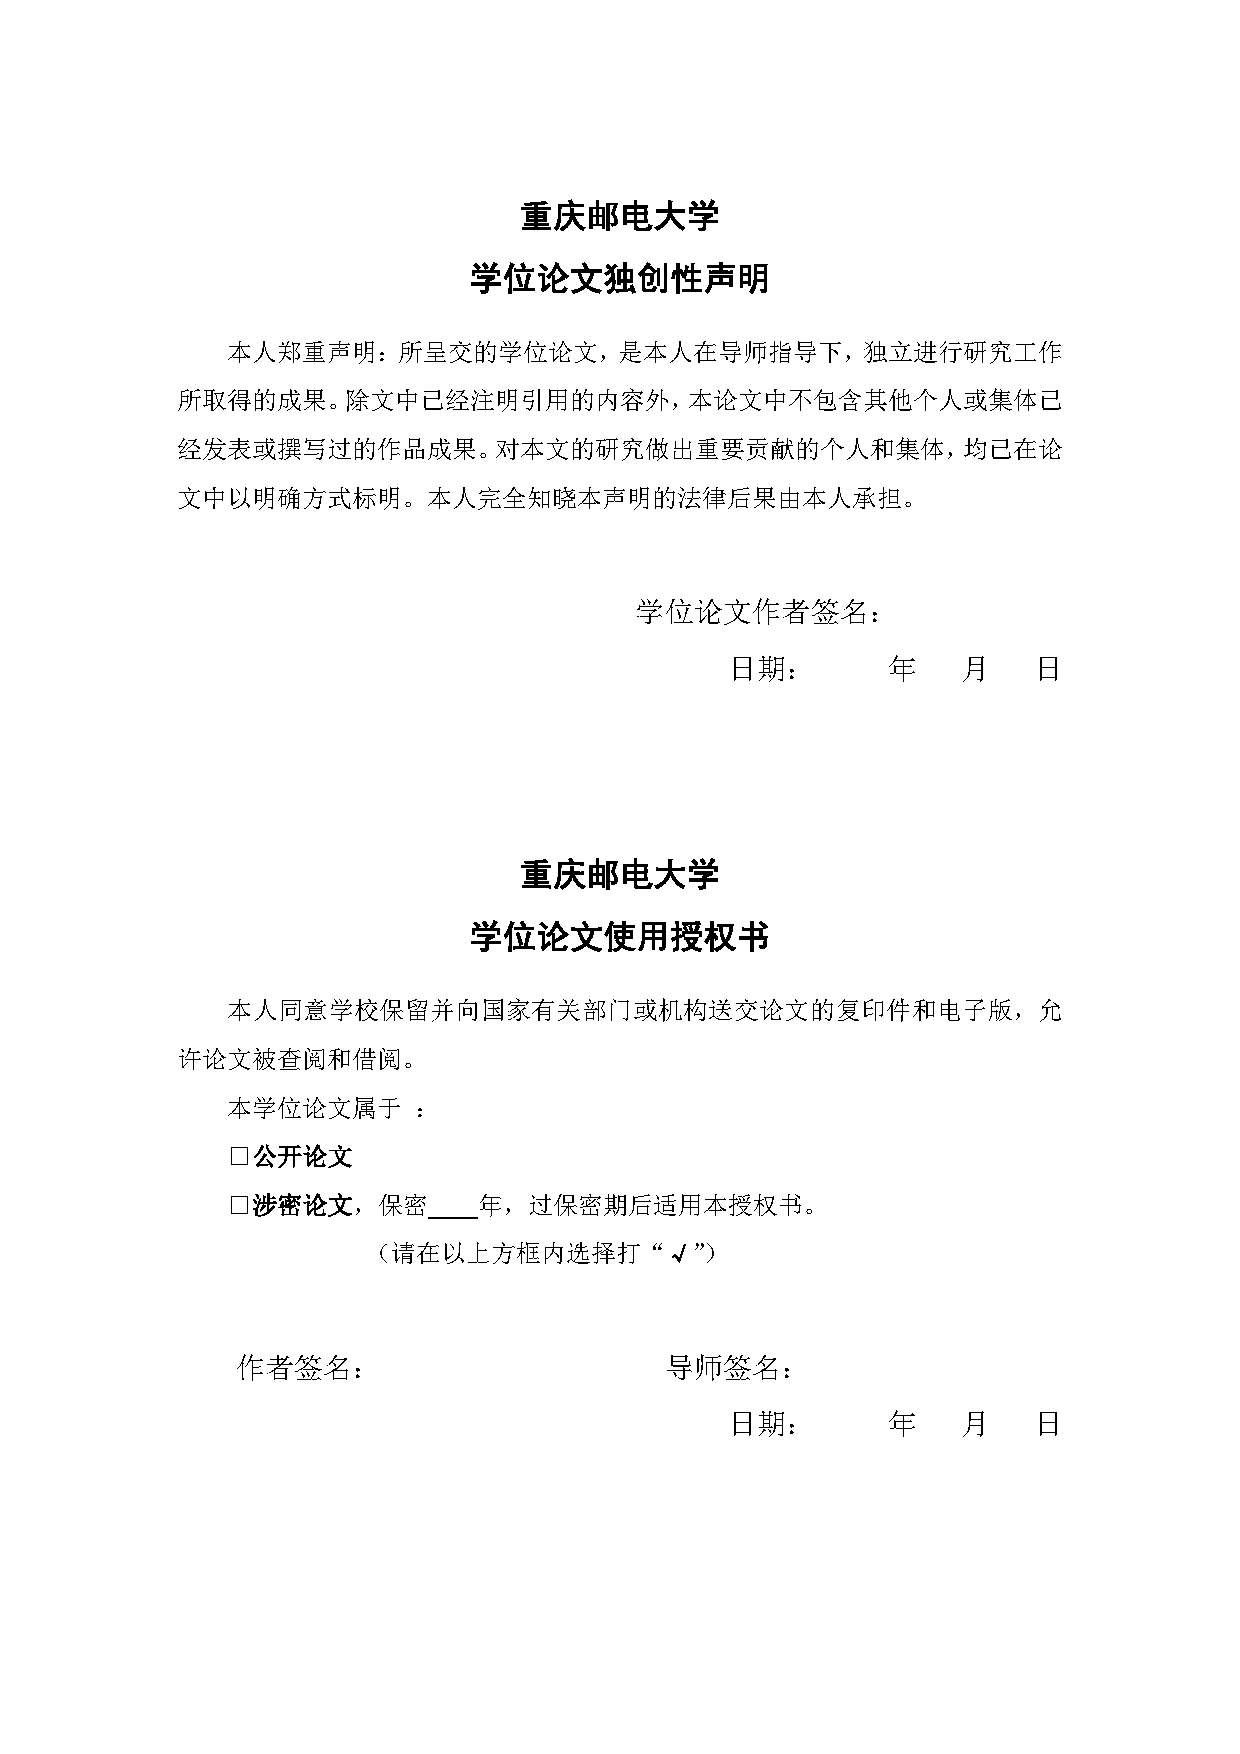
\includepdf{original.pdf}
\clearpage


\clearpage

%前序部分(中英文摘要,目录等,chapter后面不编号)
\frontmatter

%开始以大写罗马字母计页码
\pagenumbering{Roman}

\pagestyle{plain}
%页面格式
%\pagestyle{plain}

% 中文摘要页
%中文摘要,自行编辑内容



\chapter{摘\quad 要}
\xiaosi

学位论文是研究生从事科研工作的成果的主要表现,集中表明了作者在研究工作中获得的新发明、新理论或新见解,是研究生申请硕士或博士学位的重要依据,也是科研领域中的重要文献资料和社会的宝贵财富。

为进一步规范我校研究生学位论文撰写格式,提高研究生学位论文质量,参照国家标准《学位论文编写规则》(GB/T 7713.1-2006),结合我校实际,制定本模板。

  
\noindent\songti\textbf{关键词:}学位论文,撰写规范,论文模板,重庆邮电大学

\clearpage


% 英文摘要页
%英文摘要,自行编辑内容




\chapter{ABSTRACT}
\xiaosi

With the increasing demand for data privacy protection and the widespread presence of distributed data environments, federated learning (FL), as a distributed machine learning method protecting data privacy, has been rapidly developed. However, in practical applications, federated learning faces several challenges, including scarcity of labeled data, heterogeneous data distribution, and insufficient aligned samples among participating parties. Semi-supervised learning (SSL), which effectively utilizes limited labeled data and abundant unlabeled data to enhance model performance, has emerged as a significant approach to addressing these challenges. This paper focuses on federated semi-supervised learning methods and their applications in sample generation, aiming to improve the generalization ability and application value of federated learning models by fully utilizing unlabeled data and non-aligned samples under the premise of preserving data privacy. The primary research contents of this paper are as follows:

(1) To address the issue of unlabeled data absence in multi-party federated learning, a federated semi-supervised learning approach named VFPU is proposed, combining Positive-Unlabeled (PU) learning. VFPU repeatedly performs random sampling from multi-party unlabeled data, temporarily treating the sampled data as negative samples, thus forming multiple balanced training datasets (in terms of positive-negative ratio) and multiple testing datasets composed of unsampled data. Base learners are iteratively trained within a vertical federated learning framework on each training dataset. Subsequently, trained base classifiers generate predictive scores for each sample in the testing datasets. The probability of each unlabeled sample being positive is calculated based on its frequency of occurrence in the testing datasets and the sum of its scores. Samples with the highest probability are identified as reliable positive samples, then added to the positive set and removed from the unlabeled data. This iterative process of sampling, training, and selecting positives continues repeatedly. Experimental results demonstrate that the proposed method achieves comparable performance to similar non-federated approaches and outperforms other federated semi-supervised methods.

(2) To address the limited quantity of aligned samples in vertical federated learning, this paper proposes a sample generation method combining semi-supervised learning with data generation and imputation techniques. This method effectively improves data utilization and model performance by integrating federated semi-supervised learning with generative models. Specifically, the method consists of three core processes: first, cross-party feature correlations are calculated via privacy-preserving Spearman rank correlation analysis to construct a ranking system of feature association strength; second, for highly correlated features, an improved VFPU algorithm is employed for vertical federated semi-supervised learning, which iteratively generates and filters pseudo-labels, effectively leveraging unlabeled data across different tasks (classification/regression); third, for features with low correlations, generative models such as TabDDPM or VF-GAIN are introduced for data synthesis. Experiments conducted on Bank, Credit, Letter, and News datasets demonstrate that optimal performance is achieved with a correlation threshold (τ) of 0.6, a confidence threshold (α) of 0.7, and the use of GBDT as the base learner. Moreover, this method maintains stable superiority even with a sample missing rate as high as 80\%.
\\


\noindent\textbf{Keywords:} 
\begin{minipage}[t]{0.85\linewidth}
	Federated Learning; Semi-Supervised Learning; Sample Generation; Privacy Protection; Vertical Federated Learning
\end{minipage}

\clearpage


% 目录
%\begin{spacing}{1.14}
\tableofcontents


\begingroup
\renewcommand*{\addvspace}[1]{}
%图目录
%\newcommand{\loflabel}{图}
%\renewcommand{\numberline}[1]{\loflabel~#1\hspace*{1em}}
\listoffigures

%表目录
%\newcommand{\lotlabel}{表}
%\renewcommand{\numberline}[1]{\lotlabel~#1\hspace*{1em}}
\listoftables
\endgroup

%\end{spacing}





%主要符号表


\chapter{主要符号表}




\begin{table}[h]
	\renewcommand{\arraystretch}{0.6}
	\centering
	{\songti \wuhao 
	\begin{tabular}{p{2cm}p{10cm}p{1.5cm}}
		\toprule[1.5pt]
		\makecell[c]{\songti\xiaosi\bfseries 符号}&\makecell[c]{\songti\xiaosi\bfseries 说明}&\makecell[c]{\songti\xiaosi\bfseries 页码}\\
		\hline
		\makecell[c]{\wuhao ${{\mathsf{\mathcal{D}}}_{k}}$}&\makecell[c]{\wuhao 第k个数据所有者持有的数据矩阵}&\makecell[c]{\wuhao 16}\\
		\makecell[c]{\wuhao $\mathsf{\mathcal{I}}$}&\makecell[c]{\wuhao 样本ID空间,包含所有样本的唯一标识符}&\makecell[c]{\wuhao 16}\\
		\makecell[c]{\wuhao $\mathsf{\mathcal{X}}$}&\makecell[c]{\wuhao 特征空间,涵盖所有样本的全部特征维度}&\makecell[c]{\wuhao 17}\\
		\makecell[c]{\wuhao $\mathsf{\mathcal{Y}}$}&\makecell[c]{\wuhao 标签空间,包含所有可能的分类标签或类别}&\makecell[c]{\wuhao 17}\\
		\makecell[c]{\wuhao $P$}&\makecell[c]{\wuhao A方持有的正类样本集合}&\makecell[c]{\wuhao 18}\\
		\makecell[c]{\wuhao $U$}&\makecell[c]{\wuhao B方和C方共同持有的未标注数据集}&\makecell[c]{\wuhao 18}\\
		\makecell[c]{\wuhao $R$}&\makecell[c]{\wuhao 从未标注数据集$U$中成功提取出的可靠正类样本集合}&\makecell[c]{\wuhao 18}\\
		\makecell[c]{\wuhao $P_m$}&\makecell[c]{\wuhao 第m次迭代中的正样本集}&\makecell[c]{\wuhao 19}\\
		\makecell[c]{\wuhao $U_m$}&\makecell[c]{\wuhao 第m次迭代中的未标记样本集}&\makecell[c]{\wuhao 19}\\
		\makecell[c]{\wuhao $N_m^t$}&\makecell[c]{\wuhao 第m次迭代第t轮中从$U_m$随机选择的伪负样本集}&\makecell[c]{\wuhao 19}\\
		\makecell[c]{\wuhao $O_m^t$}&\makecell[c]{\wuhao 第m次迭代第t轮中的袋外样本集}&\makecell[c]{\wuhao 19}\\
		\makecell[c]{\wuhao $S_m^t$}&\makecell[c]{\wuhao 第m次迭代第t轮中基础估计器学习的输出}&\makecell[c]{\wuhao 19}\\
		\makecell[c]{\wuhao ${{\mathsf{\mathcal{P}}}_{m}}$}&\makecell[c]{\wuhao 第m次迭代中样本属于正类的概率集合}&\makecell[c]{\wuhao 19}\\
		\makecell[c]{\wuhao $R_m$}&\makecell[c]{\wuhao 第m次迭代中识别出的可靠正样本集合}&\makecell[c]{\wuhao 19}\\
		\makecell[c]{\wuhao $\mathsf{\mathcal{Y}}_{i}^{C}$}&\makecell[c]{\wuhao C方标签空间中样本i的标签}&\makecell[c]{\wuhao 19}\\
		\makecell[c]{\wuhao $\theta$}&\makecell[c]{\wuhao 可靠正样本的采样率}&\makecell[c]{\wuhao 19}\\
		\makecell[c]{\wuhao $M$}&\makecell[c]{\wuhao 最大迭代次数}&\makecell[c]{\wuhao 19}\\
		\makecell[c]{\wuhao $T$}&\makecell[c]{\wuhao 随机采样迭代次数}&\makecell[c]{\wuhao 19}\\
		\bottomrule[1.5pt]
	\end{tabular}
	}
	\label{tab:symbols}
\end{table}

\clearpage

%缩略词表




\chapter{缩略词表}
\begin{table}[h]
	\renewcommand{\arraystretch}{0.6}
	\centering
	\begin{tabular}{p{2cm}p{5cm}p{8.5cm}}
		\toprule[1.5pt]
		\makecell[c]{\songti\xiaosi\bfseries 缩写} & \makecell[c]{\songti\xiaosi\bfseries 中文} & \makecell[c]{\songti\xiaosi\bfseries 英文全称} \\
		\hline
		\makecell[c]{\wuhao FL} & \makecell[c]{\wuhao 联邦学习} & \makecell[c]{\wuhao Federated Learning} \\
		\makecell[c]{\wuhao VFL} & \makecell[c]{\wuhao 纵向联邦学习} & \makecell[c]{\wuhao Vertical Federated Learning} \\
		\makecell[c]{\wuhao HFL} & \makecell[c]{\wuhao 横向联邦学习} & \makecell[c]{\wuhao Horizontal Federated Learning} \\
		\makecell[c]{\wuhao PU} & \makecell[c]{\wuhao 正样本与未标记样本} & \makecell[c]{\wuhao Positive and Unlabeled Learning} \\
		\makecell[c]{\wuhao AE} & \makecell[c]{\wuhao 自编码器} & \makecell[c]{\wuhao Autoencoder} \\
		\makecell[c]{\wuhao GAN} & \makecell[c]{\wuhao 生成对抗网络} & \makecell[c]{\wuhao Generative Adversarial Network} \\
		\makecell[c]{\wuhao CTGAN} & \makecell[c]{\wuhao 条件表格生成对抗网络} & \makecell[c]{\wuhao Conditional Tabular Generative Adversarial Network} \\
		\bottomrule[1.5pt]
	\end{tabular}
\end{table}


\clearpage

\clearpage

%% 开始章节写作,chapter后面开始编号,显示特定页眉页脚
\mainmatter
\pagenumbering{arabic}

%正文页眉避免英文全部大写
\renewcommand\thechapter{\arabic{chapter}}
\renewcommand{\chaptermark}[1]{\markboth{第 \thechapter 章 \ #1}{}}




% 第1章


\chapter{绪论} % 创建一个新的章节,标题为“绪论”
\thispagestyle{others} % 设置当前页的页眉和页脚样式为“others”
\pagestyle{others} % 设置之后所有页的页眉和页脚样式为“others”
\xiaosi % 这是一个自定义命令,通常表示将字体设置为小四号字体(可能需要宏包支持或自定义定义)


\section{研究背景及意义}
在当今数据驱动的社会中,机器学习技术在各个领域得到了广泛应用。然而,数据隐私和安全问题日益突出,传统的集中式数据处理方式面临严峻挑战\textsuperscript{\cite{chen2021secureboost+,de2010practical}}。联邦学习(Federated Learning, FL)作为一种分布式机器学习方法,允许多个数据持有者在不共享原始数据的情况下协同训练模型,从而在保护数据隐私的同时实现模型性能的提升。在实际应用中,获取大量标记数据往往成本高昂或不可行,而未标记数据通常大量存在。半监督学习(Semi-Supervised Learning, SSL)旨在利用大量未标记数据和少量标记数据来提高模型的泛化能力。将联邦学习与半监督学习相结合,可以在保护数据隐私的同时,利用未标记数据提升模型性能\textsuperscript{\cite{li2021comatch}}。这种结合在数据分布异构、标记数据稀缺的情况下尤为重要。

在多方联邦学习中,多个数据持有者共同参与模型训练,但各自的数据特征可能不同。这种情况下,半监督学习方法的设计需要考虑数据的异构性和隐私保护。例如,某些研究提出了在多方联邦环境下的半监督学习算法,通过共享中间模型参数而非原始数据,来保护各方的隐私。在纵向联邦学习(Vertical Federated Learning, VFL)中,不同参与方拥有相同样本的不同特征。然而,实际应用中,参与方可能仅有部分样本的特征重叠,导致对齐样本不足,影响模型性能。为此,研究者提出了基于半监督学习的样本生成方法,通过生成缺失特征或伪标签,来扩充训练数据集,提高模型的泛化能力。

本研究旨在探索基于联邦半监督学习的样本生成方法,以解决数据分布异构、标记数据稀缺和对齐样本不足等问题。通过在多方联邦环境下引入半监督学习策略,设计有效的样本生成方法,可以提升模型的性能,拓展联邦学习的应用范围。这对于需要在保护数据隐私的前提下,利用分布式数据训练高性能模型的领域,如医疗、金融和智能制造,具有重要的理论和实践意义。
\section{国内外研究现状}
\subsection{联邦半监督学习}
当前的联邦半监督学习方法主要基于横向联邦架构(即参与方共享特征,但样本ID不同)。根据标注数据的位置分为标签在客户端和标签在服务器端两种情况\textsuperscript{\cite{jin2023federated}}。

(1) 标签在客户端

标注数据存于客户端,而服务器只能获取未标注数据。例如,某家公司欲利用智能手机拍摄的图片训练一个物体检测的联邦学习模型,但无法直接访问用户的本地数据,只能依赖用户的标注,如图 \ref{LabelAtClient} 所示。首先,对于不同的参与方(用户),样本ID是不同的,但参与方(用户)手机里的图片特征是一样的,所以构成了横向联邦的设置。其次,用户通常不愿为每张照片标注,给基于横向联邦的半监督学习创造了一个“客户端标注”(label-at-client)的环境。

%调整图片与上方文字之间的间距
%\vspace{-0.1cm}
\begin{figure}[h] % 开始一个图形环境,选项[ h ]表示图形尽量出现在当前位置
	\centering % 将图形居中显示
	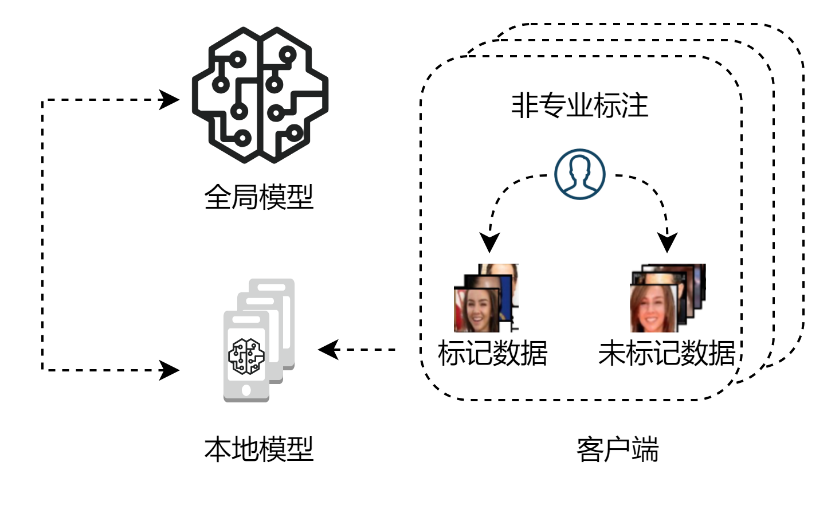
\includegraphics[width=10cm]{chapters/imgs/LabelAtClient} % 插入图像,设置图像的宽度为 10cm,图像的路径为 "chapters/31"
	\bicaption[\xiaosi 标记数据在客户端的情况] % 设置双语标题,括号中的部分是用于生成目录中的标题,设置为“小四号字体”,标题内容是“不同缩放系数v的缩放效果”
	{\wuhao 标记数据在客户端的情况} % 中文标题,设置字体为“无号”并且标题内容为“标记数据在客户端的情况”
	{\wuhao Labeled data on the client side} % 英文标题,设置字体为“无号”并且标题内容为“Labeled the data on the client side”
	\label{LabelAtClient} % 给图形一个标签,便于在文档中引用,标签为 "fig:3.1"
\end{figure} % 结束图形环境
%调整图片与下方文字之间的间距
%\vspace{-0.35cm}

RSCFed\textsuperscript{\cite{liang2022rscfed}} 主要关注联邦半监督学习中的标签隔离问题和数据异质性问题。在局部训练中,采用师生模型\textsuperscript{\cite{tarvainen2017mean}}对无标签数据进行训练。为进一步解决数据异质性问题,RSCFed 提出了子共识抽样法和距离加权聚合法。在每一轮中,通过对所有参与者的多个子集进行独立抽样,从而聚合出多个子共识模型,这样每个子共识模型都有望包含拥有标记数据的参与者。此外,本地模型会根据它们与子共识模型的距离进行加权,这样偏差模型就会得到较低的权重,其影响也会降到最低。

FedSSL\textsuperscript{\cite{fan2022private}}解决了标签隔离问题、数据隐私问题和数据异构问题。为了便于对未标记的客户端进行本地训练,FedSSL利用了伪标记技术。此外,为解决数据异构问题,FedSSL学习全局生成模型,从统一的特征空间生成数据,从而通过生成的数据缓解数据异构问题。最后,为了防止生成模型造成的隐私泄露,FedSSL利用差分隐私(DP)来限制生成模型中训练数据的信息泄露。

FedMatch\textsuperscript{\cite{jeong2020federated}}提出了一种客户端间一致性损失来解决数据异质性问题。具体来说,对每个客户端的前k个最近客户端进行采样,在每个数据样本上,本地模型的输出与前k个客户端模型的输出进行正则化,以确保一致性。此外,FedMatch还提出了分离式学习方法,将标注数据和未标注数据的参数分开,未标注数据的参数是稀疏的。更新时,只有未标记数据的客户端会上传稀疏张量,从而降低通信成本。

FedPU\textsuperscript{\cite{lin2022federated}}研究了半监督学习中更具挑战性的环境--正向和无标签学习,在这种环境中,每个客户端只有类的子集标签。在这种情况下,客户端只掌握所有类别中的一部分信息,从而导致严重的标签隔离问题。为了解决这个问题,FedPU提出了一个新颖的目标函数,即把学习客户端负类的任务交给拥有负类标签数据的其他客户端。这样,每个客户端只负责学习正类,并可自行进行局部训练。根据经验,在正类和无标签学习设置中,所提出的FedPU优于FedMatch。

AdaFedSemi\textsuperscript{\cite{wang2022enhancing}}提出了一种系统,可在联合半监督学习中利用服务器端无标记数据实现效率与模型准确性之间的权衡。在每一轮学习中,模型都是通过客户端的标注数据进行训练,并在服务器端进行汇总。服务器端未标注数据通过伪标注纳入训练过程。AdaFedSemi确定了平衡效率和性能的两个关键参数,即客户端参与率P和伪标签的置信度阈值τ。较低的P可以降低通信成本和模型准确性,而较高的τ可以降低服务器端计算成本,同时也限制了未标记数据的使用。。实验表明,AdaFedSemi通过动态调整P和τ在不同的训练阶段实现了效率和准确性之间的良好平衡。

DS-FL\textsuperscript{\cite{itahara2021distillation}}解决了与AdaFedSemi类似的问题,即客户端拥有标签数据,而服务器拥有非标签数据。它提出了一种集合伪标签解决方案来利用服务器端的非标签数据。具体来说,它不是对数据样本使用单一的伪标签,而是对所有客户端生成的伪标签进行平均,。这将创建一个客户端模型集合,并提供更好的性能。此外,由于只传输伪标签而不是模型参数,通信成本可以大大降低。此外,DS-FL发现在伪标签上进行训练会导致预测熵增大。因此,DS-FL提出了一种减少熵的聚合方法,即在聚合之前使局部输出。

(2) 标签在服务器端

标注数据存于服务器,而客户端只有未标注数据。例如,一家可穿戴设备公司希望利用联邦学习训练健康监测模型图,如图 \ref{LabelAtServer} 所示。在这种情况下,由于用户通常缺乏专业知识,无法标注健康相关数据,因此客户端的数据是未标注的。标签数据在客户端的情况比标签在服务器端设置更复杂,原因是所有客户端都只拥有未标记数据,无法为联邦模型提供额外的监督信号,仅使用无标签数据进行训练可能会导致遗忘从有标签数据中学到的知识,从而影响模型性能\textsuperscript{\cite{jeong2020federated,diao2022semifl}}。

%调整图片与上方文字之间的间距
%\vspace{-0.1cm}
\begin{figure}[h] % 开始一个图形环境,选项[ h ]表示图形尽量出现在当前位置
	\centering % 将图形居中显示
	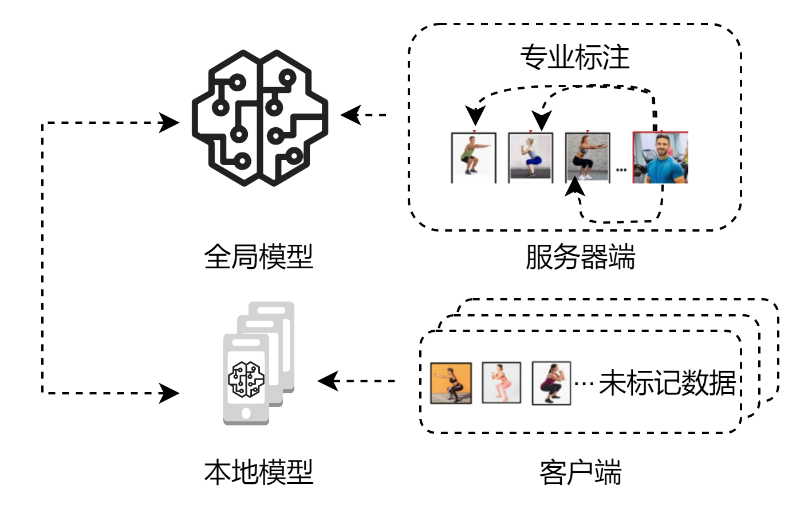
\includegraphics[width=10cm]{chapters/imgs/LabelAtServer} % 插入图像,设置图像的宽度为 10cm,图像的路径为 "chapters/31"
	\bicaption[\xiaosi 标记数据在服务端的情况] % 设置双语标题,括号中的部分是用于生成目录中的标题,设置为“小四号字体”,标题内容是“不同缩放系数v的缩放效果”
	{\wuhao 标记数据在服务端的情况} % 中文标题,设置字体为“无号”并且标题内容为“标记数据在客户端的情况”
	{\wuhao Labeled data on the server side} % 英文标题,设置字体为“无号”并且标题内容为“Labeled the data on the client side”
	\label{LabelAtServer} % 给图形一个标签,便于在文档中引用,标签为 "fig:3.1"
\end{figure} % 结束图形环境
%调整图片与下方文字之间的间距
%\vspace{-0.35cm}

为了解决标签数据和非标签数据之间的隔离问题,FedMatch\textsuperscript{\cite{jeong2020federated}}提出了一种不相干的学习方案,即分别为标签数据和非标签数据设置两套参数。在非标签数据上进行训练时,标签数据的参数是固定的,反之亦然,以防止知识被覆盖。非标记数据的参数会在参与者和服务器之间传输,而非标记数据的参数设置为稀疏的,这为通信效率带来了额外的好处。此外,为了解决不同客户端持有的异构数据问题,FedMatch 提出了客户端间一致性损失,这样不同参与者的本地模型就能在相同数据上产生相似的输出。

SemiFL\textsuperscript{\cite{diao2022semifl}}采用另一种方法来解决这些挑战。它建议使用标注数据对全局模型进行微调,以提高其质量,并减轻客户端无监督训练所造成的遗忘。此外,SemiFL建议最大限度地提高客户端模型与全局模型之间的一致性,而不是在客户端之间对模型输出进行正则化。具体来说,全局模型为客户端的未标记数据生成伪标签,而客户端的局部模型则根据伪标签进行训练。实证结果表明,与FedMatch相比,SemiFL能产生更有竞争力的结果。

(3) 联邦半监督学习方法总结

表 \ref{SummaryOfFedSemi} 总结了前文介绍的基于横向联邦的半监督学习方法,按照标签在客户端/服务器端划分。

\begin{table}[h]
	
	\centering  % 表格居中
	% 双语标题,其中中文部分用了 \songti 与 \wuhao
	\bicaption[\xiaosi \songti 联邦半监督学习方法总]
	{\songti \wuhao 联邦半监督学习方法总结}
	{\songti \wuhao Summary of federated semi-supervised learning methods}
	\label{SummaryOfFedSemi}
	
	% 使用 \resizebox 命令缩放表格到页面宽度
	\resizebox{\textwidth}{!}{
		% 整体使用 {\songti \wuhao ...} 包裹表格内容
		{\songti \wuhao
			\begin{tabular}{llllll}
				\toprule[1.5pt]
				类别 & 方法 & 半监督学习算法 & 隐私保护方案 & 数据异质问题 & 性能 \\
				\midrule
				\multirow{6}{*}{标签在客户端} 
				& RSCFed     & 教师学生模型 & 无     & 加权距离聚合   & 无                \\
				& FedSSL     & 伪标记       & 差分隐私 & 全局生成模型     & 无               \\
				& FedMatch   & 伪标记       & 无     & 客户端间一致性  & 分散学习和稀疏学习 \\
				& FedPU      & PU Learning  & 无     & 客户端间一致性  & 无                \\
				& AdaFedSemi & 伪标记       & 无     & 无             & 调整置信度阈值和参与率 \\
				& DS-FL      & 集成未标记   & 无     & 无             & 传输日志、无参数     \\
				\midrule
				\multirow{2}{*}{标签在服务器端} 
				& SemiFL     & 伪标记       & 无     & 减少熵的平均值   &                   \\
				& FedMatch   & 伪标记       & 无     & 客户端间一致性   & 分散学习和稀疏学习   \\
				\bottomrule[1.5pt]
			\end{tabular}
		}
	}
\end{table}


\subsection{数据生成方法}
生成合成数据的主要策略集中在生成模型上,这些模型旨在从现有数据集中学习丰富的表示,并随后生成新的样本。这些方法在多个领域中得到了应用,如医学研究、金融、教育和各种工业应用,其中高质量合成数据的生成对于隐私保护和有限数据集的增强都至关重要,以下将对常见的数据生成方法进行详细介绍。  
生成合成数据的主要策略集中在生成模型上,这些模型旨在从现有数据集中学习丰富的表示,并随后生成新的样本。这些方法在多个领域中得到了应用,如医学研究、金融、教育以及各种工业应用,在这些领域中,生成高质量的合成数据对隐私保护和有限数据集的增强至关重要。

基于自编码器的方法:这一类别中的先驱性工作是自编码器(Autoencoder,AE)\textsuperscript{\cite{hinton2006reducing}},其训练目的是将高维输入映射到低维潜在编码中,然后从这些编码中重构原始数据。通过强制隐藏(潜在)层降维,AE有效地学习到了压缩表示。然而,纯粹的AE是确定性的,缺乏灵活采样的直接机制。变分自编码器(Variational Autoencoder,VAE)\textsuperscript{\cite{kingma2013auto}} 通过引入概率潜在变量框架解决了这一问题,从而可以从学习到的潜在分布中采样出新的、未见过的数据点。这一扩展极大地拓宽了基于自编码器模型在合成数据生成中的潜在应用范围。在AE和VAE的基础上,Xu,Lei等人\textsuperscript{\cite{xu2019modeling}} 提出了一种针对表格数据生成和重构的改进方法。其方法更准确地建模了潜在变量与表格特征的联合分布,而后者可能包含连续和离散属性。通过关注不同类型变量之间的相互作用,该方法确保生成的合成数据忠实地反映了真实世界表格数据集(如医疗和教育数据)中存在的复杂依赖关系。

基于生成对抗网络 (Generative Adversarial Networks,GANs)\textsuperscript{\cite{goodfellow2014generative}}的方法:自2014年引入以来,GANs对生成建模领域产生了重大影响。其基本概念基于博弈论:两个网络——生成器(Generator,G)和判别器(Discriminator,D)——在对抗循环中训练。判别器学习区分真实数据和合成数据,而生成器则试图生成能够欺骗判别器的样本。当判别器无法再区分真实数据与生成数据时,这个极小极大博弈就告一段落,这表明生成器已经捕捉到了底层分布的统计特征。在GANs出现后不久,\textsuperscript{\cite{mirza2014conditional}} 提出了条件生成对抗网络(Conditional Generative Adversarial Networks,CGANs),其中生成器和判别器均基于辅助信息(如类别标签或特定输入变量)进行条件化。这一扩展框架使得生成能够针对特定类别或属性进行定向,实际上将原本的无监督设置转变为有监督或半监督范式。尽管取得了这些进展,传统GANs往往仍然面临梯度消失或模式崩溃的问题,为了解决这些问题,Banach等人用Wasserstein距离替换了Jensen–Shannon (JS)和Kullback–Leibler (KL)散度,从而诞生了Wasserstein GAN (WGAN)\textsuperscript{\cite{adler2018banach,arjovsky2017towards}}。

针对表格数据的GANs:虽然GANs最初因图像合成而受到欢迎,但它们在处理通常具有异构特征类型、不平衡和复杂依赖关系的表格数据集时,同样证明既具有挑战性又极具价值。针对这些挑战,\textsuperscript{\cite{xu2018synthesizing}} 提出了表格GAN(Table GAN,TGAN),该方法在生成器网络中应用了长短期记忆单元,并在判别器中采用了多层感知器,从而使深度架构适应于表格数据生成(例如健康记录或学生成绩数据)。2019 年,Xu, Lei等人\textsuperscript{\cite{xu2019modeling}}提出了CTGAN(Conditional Table GAN),一种专门为处理不平衡离散列、多模态连续列以及表格数据固有复杂性而设计的改进型条件GAN架构。

通过利用条件采样策略,CTGAN在建模详细分布和生成与真实数据密切对应的表格行方面表现出色。表格GANs的进一步发展,Lee等人\textsuperscript{\cite{lee2021invertible}}探索了一种可逆的表格GAN框架,该框架将对抗训练与来自可逆神经网络的负对数密度正则化相结合。该方法在训练过程中增加或降低真实样本的对数密度,从而根据隐私和质量目标生成更接近或更远离真实数据流形的合成样本。为了解决模式崩溃并提高样本多样性,Nguyen等人\textsuperscript{\cite{nguyen2017dual}}提出了一种双判别器GAN,该方法结合了KL散度和反向KL散度,以更好地捕捉真实世界数据分布的多模态特性。 Singh等人\textsuperscript{\cite{singh2021metgan}} 针对内存限制问题提出了MeTGAN,在生成器和判别器中采用稀疏线性层,从而显著降低了内存开销,而对合成质量影响不大,这在处理具有高基数类别变量的表格数据集时尤为有利。在扩展CTGAN功能方面,Zhao等人\textsuperscript{\cite{zhao2021ctab}} 提出了CTAB-GAN,能够对连续、类别和混合类型的特征进行建模。该方法能够有效处理偏态分布和多样化的特征类型,通常在与真实数据的相似性和下游任务准确性方面优于其他基线方法。 Engelmann等人\textsuperscript{\cite{engelmann2021conditional}} 提出了一种针对同时包含数值和类别变量的表格数据的条件Wasserstein GAN,通过引入辅助分类器,使模型在生成逼真合成数据的同时提升了下游任务(如信用风险评估)中分类器的性能。

基于扩散概率模型 (Denoising Diffusion Probabilistic Models,DDPMs)\textsuperscript{\cite{ho2020denoising}}的方法:与GANs一样,DDPMs因其生成高保真样本的能力而受到关注。DDPMs在多个前向步骤中系统地向数据添加高斯噪声,将原始数据分布转化为一个可处理的先验分布(例如标准正态分布)。随后,该模型通过多步马尔可夫链学习逆向(去噪)过程,逐步去除噪声以恢复数据分布。尽管DDPMs在某些领域(尤其是计算机视觉)生成了最先进的合成样本,但其多步特性可能会带来较高的计算开销。TabDDPM结合了针对表格特征混合性质精心设计的噪声添加与去除调度,同时考虑数值和类别变量的分布,展现了学习多列之间复杂关系的能力,并在生成结构化数据时缓解了纯图像中心扩散方法的缺陷\textsuperscript{\cite{kotelnikov2023tabddpm}}。

\section{论文研究的主要内容}
随着数据隐私保护需求的日益增加以及分布式数据环境的广泛存在,联邦学习(Federated Learning, FL)作为一种保护数据隐私的分布式机器学习范式得到了快速发展。然而,在实际应用中,联邦学习面临标记数据稀缺、数据分布异构以及参与方样本对齐不足等挑战。半监督学习(Semi-Supervised Learning, SSL)因其能够有效利用少量标记数据和大量未标记数据提升模型性能,成为解决上述问题的重要手段。本论文聚焦于基于联邦半监督学习的样本生成方法研究,旨在通过设计创新的算法和框架,在保护数据隐私的前提下,充分利用未标记数据和非对齐样本,提升联邦学习模型的泛化能力和应用价值。

本研究的主要内容围绕联邦半监督学习的核心问题展开,具体包括以下三个方面:首先,针对多方联邦学习中未标记数据缺失的场景,提出了一种基于多方联邦的半监督学习方法。通过分析未标记数据缺失问题(UDD-PU)的特性,设计了VFPU算法,该算法结合正样本-未标记样本(Positive-Unlabeled, PU)学习技术与联邦学习框架,利用多方协作的未标记数据提升推荐模型性能。其次,针对纵向联邦学习(Vertical Federated Learning, VFL)中对齐样本数量有限、非对齐样本未被充分利用的局限性,提出了一种基于半监督学习的样本生成方法VFPU-M-Syn。该方法通过跨方特征相关性分析、半监督预测和生成模型合成三种策略,生成高质量的伪标签和合成数据,从而扩充训练数据集,提升模型性能。最后,通过在真实数据集上的实验验证,系统评估所提方法的有效性和优越性,并分析其在隐私保护、数据异构性处理和性能优化方面的表现。

具体而言,本研究首先关注多方联邦环境下未标记数据的高效利用问题。在多方协作场景中,数据的异构性和隐私约束使得传统半监督学习方法难以直接适用。为此,本文在第3章提出了基于多方联邦的半监督学习方法VFPU,通过将PU学习技术适配到联邦学习框架中,设计了一种能够在有限标记数据条件下,利用多方未标记数据进行模型训练的算法。该方法在推荐系统等应用场景中表现出色,能够在保护数据隐私的同时,显著提升模型的精确率和召回率。

进一步地,本研究针对纵向联邦学习中对齐样本不足的问题,提出了VFPU-M-Syn方法,并在第4章进行了详细阐述。VFPU-M-Syn通过三个关键流程实现样本生成:一是计算跨方特征相关性,以识别参与方数据间的依赖关系;二是基于纵向联邦半监督学习预测未标记样本的伪标签,利用高相关性特征扩充训练数据;三是针对低相关性特征,引入生成模型合成数据,填补特征缺失,提升数据完整性。该方法不仅充分利用了对齐样本和非对齐样本,还通过隐私保护机制确保了数据安全,在小样本对齐场景下显著提高了模型的预测性能。

在实验验证方面,本研究选取了多个公开数据集,设计了一系列对比实验,分别评估VFPU和VFPU-M-Syn在不同数据分布和样本对齐程度下的表现。实验结果表明,所提方法在性能上优于传统联邦学习和半监督学习基线方法,同时在隐私保护和计算效率上具有显著优势。此外,通过对算法参数和基础估计器的分析,进一步揭示了方法设计的合理性和优化空间,为后续研究提供了理论支持和实践指导。

总之,本论文通过将半监督学习与联邦学习相结合,提出了针对样本生成的新方法,解决了联邦学习中标记数据稀缺和样本对齐不足的关键问题。这些研究成果不仅丰富了联邦半监督学习领域的理论体系,还为医疗、金融、智能制造等需要隐私保护的分布式学习场景提供了可行解决方案,具有重要的学术价值和应用前景。

\section{论文组织结构}
为清晰呈现基于联邦半监督学习的样本生成方法的研究逻辑和内容体系,本文按照科学研究的惯例组织结构,共分为五章,各章内容安排紧扣研究主题,具有明确的层次性和递进性。以下对论文的组织结构进行详细阐述:

第一章为绪论部分。本章作为全文的开篇,系统梳理了研究的背景、意义及国内外研究现状,明确了联邦半监督学习和样本生成方法的研究热点与挑战。在此基础上,简要介绍了论文的主要研究内容,并通过本节对论文结构进行概述,为读者提供研究脉络的整体框架。通过对研究背景和现状的分析,本章旨在阐明研究的必要性与创新点,为后续章节的展开奠定基础。

第二章为相关理论介绍。本章详细阐述了本文研究所依赖的理论基础和关键技术。首先介绍了联邦学习的基本概念、分类及其在隐私保护中的应用;接着论述了半监督学习的核心思想、主要方法及其在数据稀缺场景下的优势;最后探讨了表格数据生成技术的原理与应用。通过对这些理论和方法的系统梳理,本章为后续提出的算法设计提供了坚实的理论支撑。

第三章为基于多方联邦的半监督学习方法研究。本章聚焦于多方联邦学习中未标记数据缺失的问题,提出了VFPU算法。首先分析了未标记数据缺失问题(UDD-PU)的定义与特性,随后详细介绍了VFPU算法的框架设计及其在多方联邦环境下的实现流程。通过在多个数据集上的实验验证,展示了VFPU在推荐任务中的优越性能,并对实验结果进行了深入分析,最后总结了本章的研究贡献与局限性。

第四章为基于半监督学习的纵向联邦参与方样本生成方法。本章针对纵向联邦学习中对齐样本不足的挑战,提出了VFPU-M-Syn方法。本章首先分析了问题的定义与场景假设,随后系统阐述了VFPU-M-Syn的整体框架,包括跨方特征相关性计算、半监督预测和生成模型合成三个核心流程,并对算法设计与实现细节进行了详细描述。通过多组实验验证了该方法在性能提升和隐私保护方面的有效性,并对结果进行了全面分析,最后总结了本章工作的创新点与应用价值。

第五章为总结与展望。本章对全文研究内容进行了归纳总结,提炼了基于联邦半监督学习的样本生成方法的核心成果与贡献,分析了所提方法的理论意义和实践价值。同时,针对研究中存在的不足之处,如算法在极端异构数据场景下的适应性以及计算复杂度的优化空间,提出了未来工作的改进方向和展望,为后续研究提供了参考。
\clearpage



% 第2章
\chapter{相关理论介绍}
\thispagestyle{others}
\pagestyle{others}
\xiaosi

\section{本章引言}
本章旨在为后续研究提供理论支撑,系统介绍联邦学习、半监督学习和表格数据生成的基本概念、方法及其在分布式环境下的应用。首先,将阐述联邦学习的概念与分类,分析其在隐私保护和异构数据处理中的优势与挑战;其次,将介绍半监督学习的核心假设与主要方法,探讨其在标记数据稀缺场景下的适用性;最后,将讨论表格数据生成技术的原理与发展,剖析其在数据增强和隐私保护中的潜力。通过对这些相关理论的全面梳理,本章不仅为理解联邦半监督学习的样本生成方法提供了必要的知识背景,也为后续提出的算法设计和实验验证搭建了理论框架,为解决数据隐私与模型性能之间的矛盾提供了思路。

\section{联邦学习}
近几年,深度学习取得了迅猛发展,特别在人工智能和智能制造等领域展现出强大潜力。然而,数据治理和敏感信息保护等问题仍然是当前的重要挑战。为应对这些难题,联邦学习作为一种颇具前景的解决方案逐渐浮现。接下来的内容将概述联邦学习的核心概念、体系架构及训练方法。

\subsection{联邦学习概念}
联邦学习(Federated Learning, FL)是一种分布式训练方法,可在大量独立数据集上进行训练,这些数据集存储在移动电话等设备中。联邦学习采用了一种将代码嵌入数据中的方法,解决了数据隐私、所有权和数据孤岛等核心问题。在传统的集中式机器学习模式中,所有数据通常被集中存储在同一个中心服务器上进行训练与推理。然而,这种“数据集中化”的方式在实际应用中面临着多重挑战。首先是“数据孤岛”现象:不同机构或系统的数据缺乏互联互通,导致数据共享或合并分析变得困难\textsuperscript{\cite{yang2019federated}}。例如,医院之间常因合规与隐私限制而无法共享病人数据,金融机构也难以交换客户交易信息。其次是隐私与安全隐患:在大数据时代,用户产生的大量敏感信息(如医疗记录、财务数据等)被集中保存在少数服务器上,一旦发生数据泄露,将给用户和机构带来巨大损失\textsuperscript{\cite{mcmahan2017communication}}。最后,随着诸如欧盟《通用数据保护条例》(General Data Protection Regulation, GDPR)等越来越严格的数据保护法规不断出台,跨境或跨区域的数据传输受到严苛限制,集中化的数据处理模式在许多场景下已难以适用。

在这种背景下,如何既能充分利用分散的海量数据,又能有效保护数据隐私、符合合规要求,成为了机器学习领域亟待解决的关键问题。分布式数据的异构性、地理分散性以及敏感性,使得传统方法难以直接在统一服务器上进行整合和建模。针对这一问题而提出的联邦学习,为分布式数据管理与隐私保护提供了新的解决思路。

联邦学习由谷歌在 2016 年提出\textsuperscript{\cite{konevcny2016federated}},作为一个分布式学习框架,联邦学习可以使多个客户端,在本地的个体数据上共同协作配合地完成一个全局共享的模型。其中,参数 服务器协调由多轮训练迭代组成的联邦学习过程,在训练开始前,服务器初始化模 型参数并下发至全局参与的客户端\textsuperscript{\cite{mcmahan2017communication}}。参与的客户端使用其本地数据进行训练模型, 训练完成后,只将训练后得到的新模型发送回服务器。服务器从所有客户端收集这 些更新后的模型,并且对所有模型完成一次聚合,从而结束一轮迭代。由于使用分 散的本地数据完成模型训练,而不需要上传至某一设备集中处理,因此联邦学习解 决了训练任务中隐私安全的难题。具体的系统架构如图 \ref{FedArch} 所示。

\vspace{-0.1cm}
\begin{figure}[h]
	
	\centering
	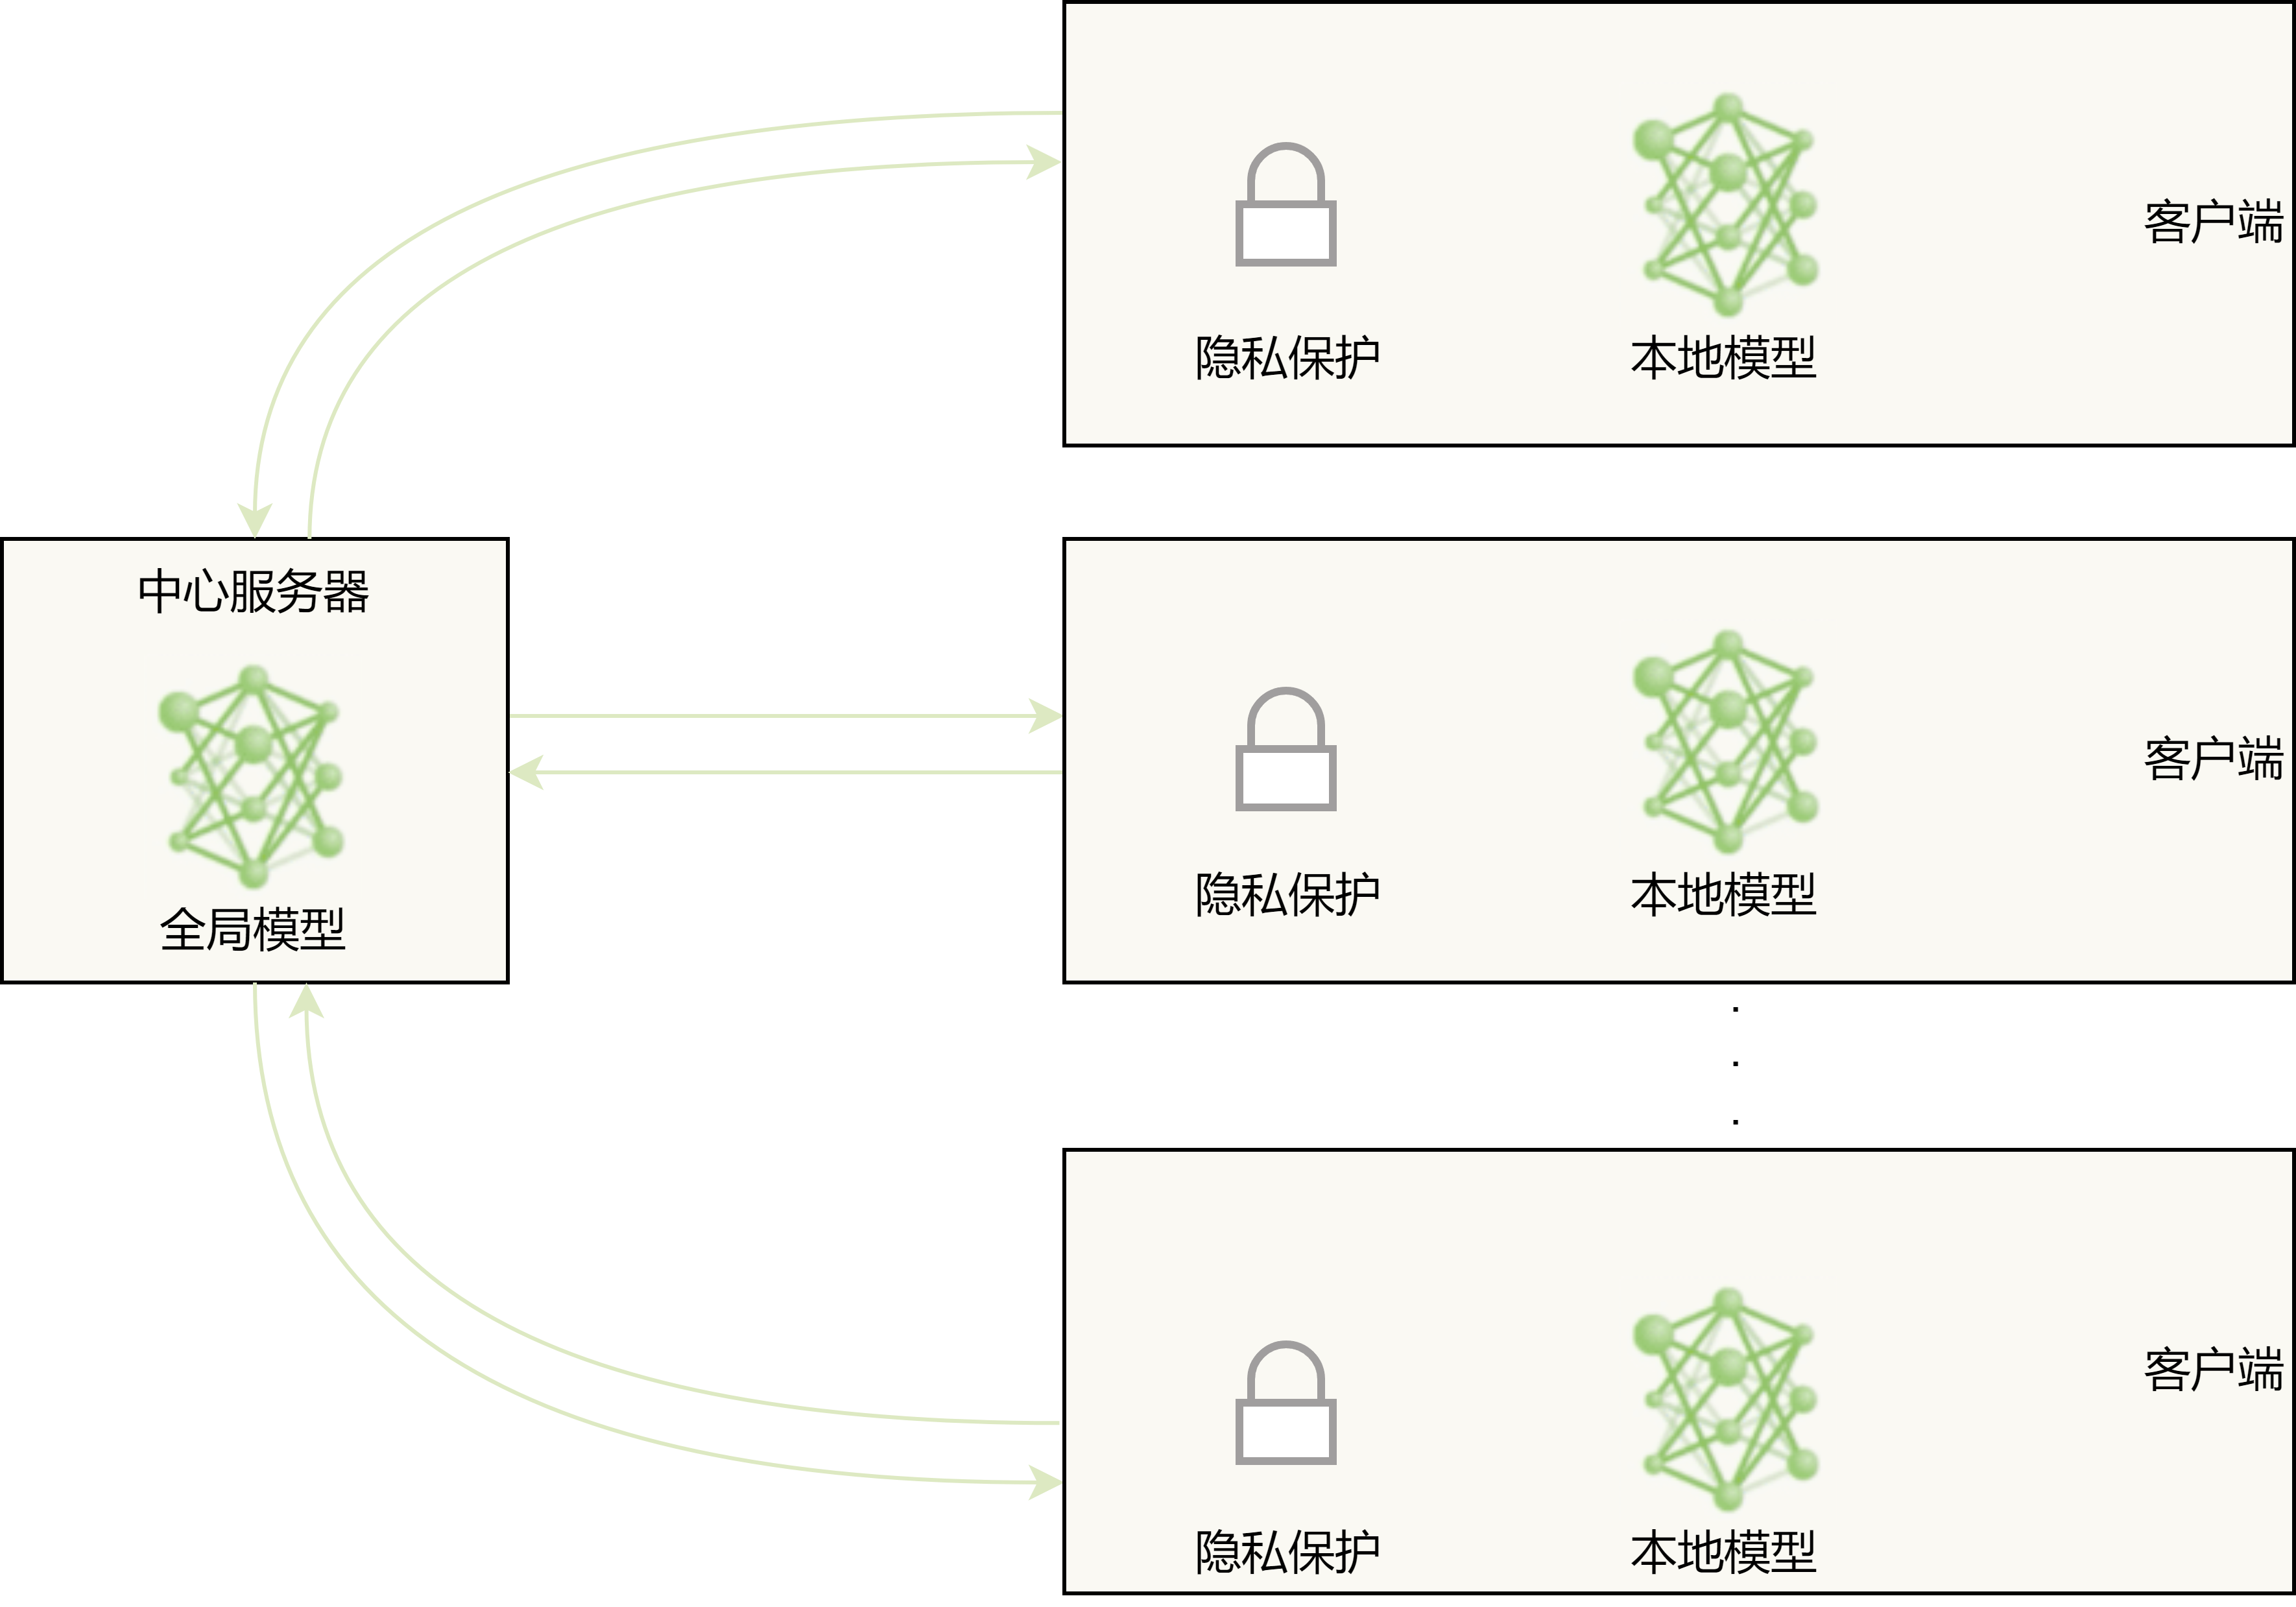
\includegraphics[width=0.9\textwidth]{chapters/imgs/FedArch7} % 插入图像,设置图像的宽度为10cm
	\bicaption[\xiaosi 联邦学习系统架构]
	{\wuhao 联邦学习系统架构}
	{\wuhao Federated learning system architecture}
	\label{FedArch}
\end{figure}
\vspace{-0.35cm}

联邦学习的核心理念是“数据在本地,模型在中央”。这一理念体现了对数据 隐私和安全的高度重视,也是联邦学习与传统中心化模型训练的最大区别。多个参与方——通常称为客户端——在不将数据集中存储的前提下,共同开发一个模型\textsuperscript{\cite{kairouz2021advances}}。该方法的一个关键特点是数据的内在异质性:由于数据仍然分布在各个客户端,各地点可用的样本往往不符合独立同分布(i.i.d.)的模式。联邦学习主要是由数据隐私、数据最小化和访问权限等问题所驱动。其应用涵盖了多个领域,包括国防、电信、物联网以及制药等。联邦学习旨在开发机器学习算法——例如深度神经网络——以便在不同节点上存储的各个本地数据集上进行训练,而无需直接交换原始数据。每个节点在自身数据上训练本地模型,并在定期的时间间隔内互相共享模型参数(例如权重和偏置)。

在整个工作流程中,中心服务器首先会初始化全局模型并将模型参数广播给所有客户端。各客户端在接收到这些参数后,利用本地数据进行训练,然后将更新后的本地模型(不包含原始数据)发送回中心服务器。聚合器再对所有客户端的模型参数进行加权平均等聚合操作,以生成新的全局模型。这个过程反复进行,直至模型收敛或达到预先设定的最大迭代次数。

联邦学习与分布式学习的主要区别在于对本地数据集特性所作假设不同\textsuperscript{\cite{konevcny2015federated}}。分布式学习旨在利用并行计算能力,通常假设每个本地数据集均为独立同分布(i.i.d.)且规模大致相同。而联邦学习则不作这些假设,它被设计用于处理异构数据,数据集的规模可能存在显著差异。此外,联邦学习中的客户端往往较为不可靠,因其通常依赖于如 Wi-Fi 等较不稳定的通信方式,并运行在电池供电的设备(如智能手机或物联网设备)上,因此面临更高的失败或中途退出风险。相比之下,分布式学习通常依赖于数据中心内的节点,这些节点具备强大的计算能力,并通过高速网络互联\textsuperscript{\cite{kairouz2021advances}}。联邦学习的核心思想是在不共享数据的情况下训练模型,仅交换模型参数。

\subsection{联邦学习分类}
联邦学习可根据特征空间和样本空间的重叠情况,主要划分为横向联邦学习(Horizontal Federated Learning, HFL)、纵向联邦学习(Vertical Federated Learning, VFL)以及联邦迁移学习(Federated Transfer Learning, FTL)\textsuperscript{\cite{yang2019federated,li2020federated}},如图 \ref{FedClass} 所示。这种划分方式能够帮助研究人员与工程实践者在不同场景下选择适宜的联邦学习方案,从而更高效地利用分布式数据进行模型训练。

当两类参与方之间的用户维度之间存在较少的重叠而用户数据特征之间重叠 存在较多时,称之为横向联邦学习场景\textsuperscript{\cite{yang2019federated,liu2019communication}},如图 \ref{FedClass}\subref{FedClassA} 所示。例如同一家银行系统,但存在不同地区之 间的业务,此时银行不同地区之间的用户基本没有重叠,但之间的业务内容信息却 类似,隐私可以采用联邦学习来进行深度学习任务。

与之相对,纵向联邦学习(VFL)则适用于样本空间高度重叠,但特征集差异较大的场景\textsuperscript{\cite{liu2020secure,chen2020vafl}},如图 \ref{FedClass}\subref{FedClassB} 所示。例如,某些银行与电商平台在用户群体上可能有很大交集,却掌握了不同维度的用户信息:银行侧有用户财务信用数据,电商侧则有用户消费行为数据。在这种情形下,联合建模可以充分利用双方不同来源的特征信息,从而获得更全面、更准确的刻画。当各方在训练过程中只需对对齐后的公共用户进行联合梯度更新时,无需共享原始数据,依然能够保证个人隐私与数据安全。

\vspace{-0.1cm}
\begin{figure}[h]
	\centering
	\subfigure[]{
		\label{FedClassA}
		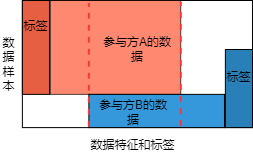
\includegraphics[width=0.3\textwidth]{chapters/imgs/FedClassA}}
	\hspace{0.01\textwidth}
	\subfigure[]{
		\label{FedClassB}
		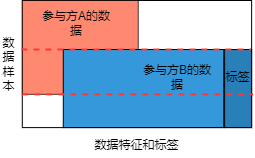
\includegraphics[width=0.3\textwidth]{chapters/imgs/FedClassB}}
	\hspace{0.01\textwidth}
	\subfigure[]{
		\label{FedClassC}
		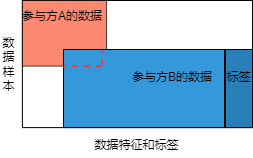
\includegraphics[width=0.3\textwidth]{chapters/imgs/FedClassC}}	
	\bicaption[\xiaosi \songti 联邦学习分类]
	{\centering \wuhao 联邦学习分类。(a) 横向联邦学习;(b) 纵向联邦学习;(c) 迁移联邦学习}
	{\centering \wuhao Federated Learning Classification. (a) Horizontal Federated Learning; (b) Vertical Federated Learning; (c) Transfer Federated Learning}	
	\label{FedClass}
\end{figure}
\vspace{-0.35cm}

第三种形式是联邦迁移学习(FTL),其特点在于样本空间与特征空间均不完全重叠\textsuperscript{\cite{yang2019federated,chen2020vafl}},如图 \ref{FedClass}\subref{FedClassC} 所示。在部分数据量较少或者特征不足的场景里,可以通过迁移学习的方法来补充数据或特征不足的问题。此时,不同组织或机构拥有的用户群体与特征集合可能仅存在少量重叠,但依然可通过联邦迁移学习的思想,将部分预训练模型的知识进行迁移,从而提升任务的性能或模型的泛化能力。这种方法特别适用于小样本或垂直领域知识不足的情景,有效地拓展了联邦学习在更多应用场景下的可行性。

综上所述,横向联邦学习、纵向联邦学习及联邦迁移学习分别应对了特征空间或样本空间上的不同重叠情况。它们在数据类型、业务场景和技术实现上各有侧重,却都遵循了联邦学习的核心理念:在不直接交换数据的前提下,实现多方协作与知识共享。这种多元化的联邦学习形式为不同行业和应用需求提供了灵活的选择,也在隐私保护和跨域协作方面展现出巨大的潜力。
\section{半监督学习}
本节将介绍半监督学习的基本概念,详细讨论几种半监督学习的方法,包括伪标签生成方法和PU(Positive and Unlabeled)学习。
\subsection{半监督学习概念}
在实际任务中,有标注数据往往十分稀缺,且标注过程需要投入大量的人力与时间成本。然而,大量的未标注数据通常容易获取,如果能够加以有效利用,便能显著提升模型的学习性能\textsuperscript{\cite{2015Semi}}。

半监督学习的核心思想在于同时利用少量标注数据与大量未标注数据进行联合训练,从而提升模型的泛化能力\textsuperscript{\cite{van2020survey}}。通过对未标注数据的“挖掘”或“自学习”,半监督学习有效弥补了标注样本不足所带来的数据缺陷\textsuperscript{\cite{van2020survey}}。

半监督学习的理论构建通常基于以下三个假设:(1)平滑性假设(Smoothness Assumption),该假设表明,在特征空间里,若两个样本的距离较为接近,那么它们所对应的标签也大概率相近。(2)聚类假设(Cluster Assumption),此假设指出,处于同一簇内的样本往往具有相同的标签,即样本会依据标签的一致性形成自然的聚类。(3)低密度分隔假设(Low - density Separation Assumption),该假设认为,不同类别的样本集合之间由低密度区域分隔开来,这些低密度区域就像天然的“屏障”,将不同类别的样本清晰划分。

与监督学习相比,半监督学习更加强调对未标注数据的有效利用;而与无监督学习相比,半监督学习则依靠少量标注样本对模型进行指导,使模型能够在庞大的未标注数据中学习到更具区分度的特征\textsuperscript{\cite{van2020survey}}。
\subsection{半监督学习方法}

(1) 伪标签生成方法

该方法基于自训练(Self-training)假设\textsuperscript{\cite{lee2013pseudo}},通过为未标记数据生成伪标签来实现半监督学习,并将这些伪标签作为额外的训练数据。未标记数据对应的损失项通常可以表示为:
\begin{equation}\label{eq:2-1}
	L_u = \frac{1}{n} \sum_{i=1}^{n} \sum_{j=1}^{K} R \Bigl( y_i^{j}, \, p(x_i \mid \theta) \Bigr)
\end{equation}
式中,$ p(x_i \mid \theta) = \mathrm{softmax}\bigl(f(\theta, x_i)\bigr) $ 为模型 $ f(\theta) $ 在样本 $ x_i $ 上的预测概率分布,而 $ y_i^{j} $ 则指生成的伪标签,可以是独热编码或概率向量。为了实现熵最小化,通常采用独热编码的形式,使模型在预测时更加自信,从而将决策边界放置在低密度区域。当使用软标签时,为了达到类似的熵最小化效果,往往会对伪标签进行锐化处理,例如采用 0-1 阈值化:
\begin{equation}\label{eq:2-2}
	y_i^{j} = \mathrm{argmax}\Bigl(p(\theta', x_i)\Bigr)
\end{equation}
即直接以当前模型的预测作为伪标签。

在公式 \eqref{eq:2-2} 中,$ R(\cdot, \cdot) $ 表示用于度量差异的距离函数,常用的包括均方误差(MSE)或交叉熵等\textsuperscript{\cite{van2020survey}}。为了进一步保留那些置信度较高的伪标签样本,可对公式 \eqref{eq:2-1} 进行更深层次的优化,通过引入一个筛选函数 $\mathrm{Filter}(\cdot)$ 来实现:
\begin{equation}\label{eq:2-3}
	L_u = \frac{1}{n} \sum_{i=1}^{n} \sum_{j=1}^{K} 
	\mathrm{Filter} \Bigl( R \bigl( y_i^{j},\, p(x_i \mid \theta) \bigr) \Bigr)
\end{equation}
使得模型仅聚焦于高可信度的伪标签样本。

此外,为了构建总的目标函数,常将带标签数据上的监督损失与未标记数据上的伪标签损失结合,得到:
\begin{equation}\label{eq:2-4}
	L = L_s + \alpha \, L_u
\end{equation}
式中,$ \alpha $ 用于平衡两部分损失,既可视为一个固定超参数,也可以随训练迭代而动态调整(如 $\alpha = \alpha(t)$)。通过对 $ L $ 的梯度进行反向传播并更新模型参数,模型会在每次迭代中不断重新预测未标记数据的伪标签,从而持续提升模型对未标记数据的刻画能力,直至收敛或满足预设的终止条件。


(2) PU(Positive and Unlabeled)学习

PU学习是一种有效的半监督学习策略,旨在仅依赖少量确证的正例样本与大量未标注数据来构建分类模型,而无需明确的负例样本\textsuperscript{\cite{elkan2008learning,mordelet2013bagging}}。在传统的二分类场景中,研究人员通常需要完整且平衡的正负例数据集以训练模型。然而,随着数据规模的指数级增长,人工标注的成本与难度显著上升,大量真实世界数据缺乏可靠标记。为应对这一挑战,PU 学习通过将未知标签样本纳入训练过程,减少对全面标注的依赖,同时利用少量的正例样本来学习准确的决策边界。

近年来,PU 学习方法在多个领域均展现出卓越潜力。与传统方法相比,PU 学习无需显式负例,也能有效定位负类分布或异常模式,并对类别不平衡问题进行修正\textsuperscript{\cite{elkan2008learning}}。此外,PU 学习对大规模未标注数据的需求大幅降低了标注成本,尤其适合工业监测与异常检测等场景:在此类应用中,异常事件极为稀少,未标注数据往往代表了正常状态,因此仅使用少量正例便可使算法逐步“发掘”潜在负类特征,从而显著提升分类器的稳健性。

一种直接而高效的方法是将已标记的正例样本视为正类,而将未标注样本简单地视为负类进行训练\textsuperscript{\cite{elkan2008learning}}。尽管这一策略在理论上可能显得过于简化,但已有研究表明它仍能取得令人满意的实验效果。根据 Elkan 与 Noto\textsuperscript{\cite{elkan2008learning}} 的理论,当满足一定假设(例如正例样本是随机抽取的标注数据)时,仅基于正例与未标注数据训练得到的分类器,其输出分数与使用完整正负例数据训练的分类器之间存在正比关系。因此,在对样本进行排序或评估其成为正例的可能性时,这种简单方法的排名性能可与使用完整标注数据训练的模型相媲美。

进一步地,Mordelet 与 Vert\textsuperscript{\cite{mordelet2013bagging}} 提出了针对PU学习的改进袋装法(PU Bagging)。该方法首先在构建训练集时采用自助采样策略,即保留所有正例样本,并从未标注数据集中有放回地随机抽取一部分样本作为伪负例;随后利用“正例+伪负例”的自助样本训练分类器,并将训练好的分类器应用于未参与本轮自助抽样的未标注样本,记录这些袋外样本的预测得分;最后通过重复上述自助采样与训练过程,每个未标注样本将获得多个袋外预测分数,并以这些分数的平均值作为最终预测结果。

实验表明,当正例样本数量稀少或者未标注数据中负类比例本就较低时,PU Bagging方法往往表现优异,甚至能够超越某些更复杂的PU学习算法。此外,由于PU Bagging方法在处理大规模未标注数据时具备较高的计算效率,更适用于实际工业场景中的在线或分布式训练需求。

目前,多数 PU 学习算法通常可以归纳为 “两步法”,其主要步骤:首先进行可靠负样本识别,从未标注数据中筛选出高置信度的负例子集。尽管其规模可能较小,但标签质量较高,为后续训练提供基准。接着进行迭代分类器训练,将已知正例与前一步识别的可靠负例合并训练初始分类器,然后将该分类器应用到剩余的未标注数据。这个过程通常会进行多次迭代,随着更多可靠负例被标识并加入训练集,分类器的决策边界不断得到精炼,直至满足停止准则或取得收敛。

虽然两步法在机制上与 Shubham Jain 的 “伪标签” 策略相似,但其针对 PU 问题进行了专门设计,通过动态更新和扩充可靠负集来逐步提升分类器性能。相比于一般的半监督学习,两步法在 PU 场景下更强调对未知类别分布的主动探索,因而能在缺乏负例注释的环境中持续改进模型的判别能力。
\section{表格数据生成}
表格数据生成(Tabular Data Generation)是指通过一定的算法或模型,基于现有真实数据或先验知识,合成出具有与真实数据相似统计分布和特征的虚拟表格数据。随着大数据时代的到来与隐私保护需求的不断增长,表格数据生成技术在医疗、金融、电商、社交媒体等领域具有越来越重要的应用价值。该技术不仅可以用于数据增强(Data Augmentation)和算法测试,还能够在保证隐私安全的前提下,为数据分析和机器学习模型提供更多的训练样本\textsuperscript{\cite{li2021survey}}。

表格数据生成技术的核心目标在于在保持数据特征分布与关联关系的同时,最大程度地提升所生成数据的真实性与多样性,其典型生成过程需要综合考虑多个方面。生成数据需与真实数据在数值特征和类别特征上保持相似的分布特征,以避免重要特征的偏差或缺失,同时在多列或多特征维度的表格数据中捕捉并保留不同字段间复杂的相关性\textsuperscript{\cite{zhang2020tab}}。此外,生成过程还需兼顾隐私保护,既要避免暴露个体敏感信息,又要保证数据的可用性和真实性,而为了满足大规模数据需求,生成技术的效率和可扩展性也成为重要的考量指标。

当前,针对表格数据的生成方法主要分为基于统计模型和基于深度生成模型两大类,前者通过参数化或非参数化的统计分布对真实数据进行建模,后者则更多依赖神经网络,尤其是生成对抗网络(GAN)和变分自动编码器(VAE)等框架来生成高维度和多样化的数据\textsuperscript{\cite{brown2019differential}}。基于统计模型的方法通过对单变量分布及变量间相关关系建模,能够生成近似真实分布的数据,实现简单且具备一定可解释性,但在数据相关性复杂或维度较高时容易出现失配。而近年来,GAN 和 VAE 等深度生成模型在图像、文本等领域取得显著成果后,也逐渐应用于表格数据生成。通过生成器与判别器间的对抗训练,这类方法能捕捉多维特征关系并生成高保真合成数据,然而通常需要大量样本训练,且在超参数选择与模型可解释性方面仍面临较大挑战。

\section{本章小结}
本章系统介绍了联邦学习、半监督学习以及表格数据生成方法的核心理论与技术,为后续算法设计和实验分析奠定了基础。针对分布式环境下的数据隐私和标记数据稀缺问题,本章分别从联邦学习、半监督学习和表格数据生成三个方面展开讨论。

首先,回顾了联邦学习通过分布式协作实现数据隐私保护与模型优化的基本思想,具体分析了横向联邦、纵向联邦和联邦迁移学习在异构数据处理与样本对齐中的优势与挑战。其次,阐述了半监督学习利用少量标记数据与大量未标记数据进行学习的基本范式,重点介绍了伪标签生成和PU学习方法,为联邦学习框架下的半监督技术提供支持。最后,讨论了基于统计模型和深度生成模型的表格数据生成技术,强调其在数据扩充和隐私保护方面的潜力,为解决联邦学习中的样本不足与特征缺失问题提供了思路。

综上所述,本章明确了联邦学习、半监督学习和表格数据生成技术在解决数据隐私和性能优化问题中的协同作用,为后续提出的 VFPU 和 FedPSG-PUM 等方法奠定了理论和技术基础。下一章将进一步探讨基于多方联邦的半监督学习方法,分析其在未标记数据缺失场景中的应用与表现。


% 第3章
\chapter{基于多方联邦的半监督学习方法} % 定义章节,章节标题为“图表、公式格式和印制要求Abc”

\thispagestyle{others} % 设置当前页面的页眉页脚样式为“others”,该样式需要用户自行定义

\pagestyle{others} % 设置后续页面的页眉页脚样式为“others”,该样式同样需要用户自行定义

\xiaosi % 可能是自定义的命令,通常用于调整字体大小或格式,需要在前文定义


\section{本章引言}
联邦学习(Federated Learning, FL)作为一种新兴的分布式机器学习方法,为多方协作数据隐私保护问题提供了一种解决方案\textsuperscript{\cite{mcmahan2017communication}}。联邦学习允许多个数据所有者(客户端)在不共享原始数据的前提下,通过交换模型参数或梯度实现联合训练。现有联邦学习方法主要集中在监督学习场景,但在现实中,由于标注成本高、领域专家稀缺或资源受限等原因,数据往往并不完全标记。因此,近年来研究者开始探索半监督学习(Semi-Supervised Learning, SSL)在联邦学习场景下的应用,特别是仅包含正样本和未标记数据的PU(Positive and Unlabeled)学习问题。目前已有一些代表性方法被提出,如:FedPU算法\textsuperscript{\cite{lin2022federated}}通过PU学习策略提高有限标记数据的联邦学习性能;RSCFed算法\textsuperscript{\cite{liang2022rscfed}}通过聚合多个子共识模型以处理本地客户端的非独立同分布(Non-IID)问题;FedMatch算法\textsuperscript{\cite{jeong2020federated}}优化客户端间参数一致性与分解策略,改善有限标记数据下的联邦学习效果;AdaFedSemi算法\textsuperscript{\cite{wang2022enhancing}}则借助多臂赌博机优化客户端参与度与伪标签质量,提升半监督联邦学习的性能。

上述场景属于纵向联邦学习(Vertical Federated Learning, VFL)\textsuperscript{\cite{yang2019federated}},即多个数据所有者共享相同的样本ID空间,但特征空间不同。尽管纵向联邦学习在隐私保护机器学习领域具有重要的应用价值,但当前针对VFL场景下的半监督学习研究仍然较为稀少,尤其是在PU(正样本-未标记)学习问题上的探索几乎处于空白状态。

在纵向联邦学习的实际应用中,往往存在这样一种特殊的PU学习问题:数据分布方面,不同的数据所有者(机构)拥有部分重叠的样本ID,但特征空间不重合且各方数据具有专有性;数据类型方面,通常目标方仅持有标记为正类的数据,其他参与方则仅持有未标记数据,并且所有方之间无法直接访问对方的原始数据;在这种情形下,各方希望联合训练一个有效的机器学习模型,用于从未标记数据中精准识别出可靠的正样本,同时保证各自数据的隐私安全。

这种场景中,目标方只拥有正样本,而其他方仅拥有未标记数据,恰好对应了PU学习问题的典型特征,即仅凭正样本和未标记数据来构建有效的分类模型。然而,现有的PU学习方法\textsuperscript{\cite{mordelet2014bagging, liu2003building, liu2015classification, xu2017multi}} 一般都默认正样本和未标记数据在训练过程中可以同时访问,而在VFL场景下,由于数据分布于不同的机构之间并且无法直接共享,这种传统PU学习框架无法直接适用于该场景。这导致了一个全新的挑战,即未标记数据缺失的PU学习问题(Unlabeled-Data-Deficient PU, UDD-PU)。

为应对这一挑战,本章提出了一种新的方法,即纵向联邦正样本-未标记学习(Vertical Federated Learning with Positive and Unlabeled data, VFPU)。VFPU允许多个数据所有者在不暴露自身原始数据的前提下,通过协作训练一个联合模型,实现在未标记数据中有效识别正样本。VFPU方法在保障数据隐私的基础上,仅通过交换加密后的中间计算结果完成联邦训练过程;同时,该方法融合了PU学习策略,能够在纵向联邦学习场景下充分利用未标记数据,提升模型的分类性能。此外,VFPU具备广泛的应用前景,能够有效应对金融、医疗、智能制造等多个领域的数据孤岛问题,满足实际应用中日益严格的数据隐私保护要求。

本章后续的结构安排为:3.2节将分析并详细定义UDD-PU问题;3.3节将系统阐述多方联邦半监督学习的具体问题定义和整体方法框架,深入介绍VFPU方法的执行流程与算法设计,并在多个真实数据集上开展实验验证与分析;最后,3.4节对本章研究成果进行总结归纳。



\section{问题分析与定义}
在本章节讨论的语境中,首先探讨一个分布式数据场景:K个独立的数据所有者各自掌控着大型数据集的不同部分,并存在一个中央服务器作为协作协调者。每个数据所有者持有的数据被系统地组织成矩阵形式,具体记作${{\mathsf{\mathcal{D}}}_{k}}$(下标k表示第k个数据所有者)。该矩阵中,每行对应一个独立样本(即具体的数据实例或观测值),每列对应特定特征(即样本的可测量属性或特性)。从全局视角,整个分布式数据集可抽象为结构化三元组$(\mathsf{\mathcal{I}}, \mathsf{\mathcal{X}}, \mathsf{\mathcal{Y}})$,其中:$\mathsf{\mathcal{I}}$为样本ID空间,包含所有样本的唯一标识符;$\mathsf{\mathcal{X}}$为特征空间,涵盖所有样本的全部特征维度;$\mathsf{\mathcal{Y}}$为标签空间:包含所有可能的分类标签或类别。

在传统纵向联邦学习(Vertical Federated Learning, VFL)框架中,通常存在一个关键假设:至少有一个参与方持有其数据部分的完整标签集,从而能够实现有监督的预测模型训练。然而,这一假设在大量现实场景中往往难以成立,因为获取全量标注数据集面临严峻挑战。这种挑战主要源于实际商业环境中的多重约束,包括但不限于:隐私保护法规对数据使用的限制、高昂的人工标注成本、行业竞争导致的数据孤岛现象、敏感信息共享的法律风险以及动态数据更新带来的标注滞后问题。

为了更清晰、更具体地理解这一概念,现在考虑一个具体的示例场景,其中涉及三位不同的数据拥有者,将其分别称为 A 方、B 方和 C 方。这三方各自持有敏感数据——这些信息对其业务至关重要,但由于隐私和安全方面的考虑,他们不愿直接公开。因此,他们需要在确保数据隐私严格保护的前提下,以安全的方式进行合作,充分利用各自的数据资源。

在该场景中,所涉及的数据样本可以被划分为两大基本类别:正类(positive)和负类(negative),这可以对应于某些应用场景中的理想(或期望)行为与非理想(或不期望)行为。一个值得注意的特点是,这三方在样本标识符(ID)上存在一定程度的重叠,即某些样本可能同时出现在多个参与方的数据集中,但每一方所收集或观察到的特征可能有所不同。

具体而言,A 方持有一个样本集合,记作 $ P $,该集合的独特之处在于它仅包含正类样本——即被明确标记为正类的数据实例,不包含任何负类或不确定的样本。而 B 方和 C 方共同持有一个未标注数据集,记作 $ U $,其中的样本类别(正类或负类)未知。需要特别强调的是,$ U $ 不包含 A 方数据集 $ P $ 中的任何样本,即 $ U $ 是一个独立的数据集,不与 A 方的正类样本重叠。

这三方的主要目标是通过合作共同训练一个推荐模型,该模型的作用是分析未标注数据集 $ U $,并从中识别出可以被可靠归类为正类的样本。这一过程的输出结果记作 $ R $,即从 $ U $ 中成功提取出的可靠正类样本集合。一旦这些样本被识别出来,$ R $ 将被提供给 A 方,使其能够基于这些推断出的正类实例向客户或用户提供精准的产品推荐,从而提升其业务能力和市场竞争力。

该问题设置引入了一个重大挑战,使得传统的纵向联邦学习(VFL)算法在其标准形式下无法适用。核心问题在于,参与的各方——A 方、B 方和 C 方——都不拥有完整的标签数据。在传统的 VFL 方案中,至少需要有一方持有完整的标注数据,以便模型能够从监督信号中学习,并在联邦系统中传播。然而,在本问题中,A 方仅拥有正类样本的标签(即数据集 $ P $),而 B 方和 C 方的数据集 $ U $ 完全没有标签,这导致了一个关键的缺口,使得标准的 VFL 技术无法直接应用。

为了解决这一挑战,可以考虑采用半监督学习(semi-supervised learning)策略,该策略专门用于处理包含部分标注数据和未标注数据的场景。在本问题背景下,一个特别相关的方法是PU 学习(Positive and Unlabeled learning,正类与未标注学习)。PU 学习是一种特殊的半监督学习技术,它利用一组带有正类标签的样本($ P $)和一组未标注样本($ U $)进行训练,目标是在未标注数据集中识别出正类实例。PU 学习特别适用于缺少负类标签或负类标签不可靠的情况,因此在本问题中具有较大的应用潜力。

然而,PU 学习在本场景下的直接应用存在一个关键限制:传统的 PU 学习方法假设学习者可以同时访问 $ P $ 和 $ U $,从而能够直接对比正类样本和未标注样本,并进行有效的训练。然而,在本联邦学习场景中,这一假设并不成立,因为 A 方仅持有 $ P $,而 $ U $ 分布在 B 方和 C 方手中。由于隐私保护的要求,各方无法简单地将数据汇总到一个集中存储库,也不能自由共享数据给 A 方,这使得传统 PU 学习方法难以直接应用,成为本问题的一个重要挑战。

在这种情况下,A 方希望将推荐服务集成到其业务运营中,但面临一个全新的复杂挑战,将其称为“未标记数据缺失的 PU 学习问题”(Unlabeled-Data-Deficient PU, UDD-PU)。该问题的核心特征在于,A 方仅能访问正类样本集 $ P $,但无法直接获取未标注数据 $ U $,这使得传统的 PU 学习方法无法直接应用。此外,由于数据在联邦学习环境下分布——即 $ U $ 分散存储在 B 方和 C 方手中——并且所有参与方都施加了严格的隐私保护要求,因此现有的 PU 学习方法若不进行重大改进,无法直接适用于该场景。

因此,UDD-PU 问题代表了联邦学习、半监督学习和隐私保护计算的独特交汇点,需要创新性的解决方案,以便在这些约束条件下实现有效的协作和模型训练。

总的来说,这一扩展解释突出了该场景的复杂性、传统方法的局限性,以及新问题的提出,为进一步的研究探索或方法论发展奠定了详细的基础,可用于撰写相关研究论文。


\section{基于多方联邦的半监督学习方法}
在推荐系统中,有效利用多个参与方的数据,同时应对特定挑战至关重要。在某些场景下,会出现 UDD-PU 学习问题,即某一方(在本例中为 A 方)缺乏足够的未标记样本,导致无法使用传统的正例-未标记(PU)学习技术来有效训练推荐模型。这种未标记数据的不足会影响模型的泛化能力,导致性能下降和推荐结果不够准确。为了解决这一问题,本章提出了 VFPU 算法,这是一种结合了纵向联邦学习框架与 PU 学习技术的新方法。VFPU 旨在解决 A 方未标记样本不足的问题,通过更好地利用分布式数据资源,提升推荐模型的性能。

在本章中,基于 VFPU 的推荐过程主要包括三个核心步骤:数据预处理、加密样本对齐以及 VFPU 算法的执行。这些步骤共同构成了一个稳健的流程,以在隐私保护的协作环境中提升推荐的准确性。VFPU 的主要目标是在多个参与方持有的未标记数据集中识别可靠的正例样本。通过精准定位这些可靠的正例样本,模型能够更好地区分正例和负例,即使在缺乏明确标注的负例数据的情况下——这是 PU 学习场景中的常见挑战。

这一能力在推荐系统中尤为关键,因为用户偏好通常是通过交互隐式表达的,而非通过显式标签标注。因此,模型需要从有限或噪声较大的数据中推断用户偏好。通过识别这些可靠的正例样本,模型能够更深入地理解正例实例的特征,例如用户偏好或产品相关性,从而最终生成更准确、更个性化的产品推荐,以满足 A 方的需求。

对于 A 方而言,由于数据资源有限,其推荐模型的性能可能受到约束。然而,通过这一联邦学习方法,A 方可以利用 B 方和 C 方的丰富数据集,从而显著增强推荐模型的稳健性。同时,确保数据隐私的保护,并促进多个参与方之间的无缝协作,严格遵循联邦学习的核心原则。在整个过程中,数据隐私得到了精心维护,每个参与方的原始数据始终保持本地化,仅共享模型更新或聚合后的信息,而不会泄露敏感的个人记录。

这种隐私保护的协作方式在 图 \ref{fig:VFPU} 中得到了展示,该图详细说明了推荐过程的具体流程。本章的后续章节将对这一过程中的各个步骤进行深入探讨,以提供对该方法的全面理解。

\vspace{-0.1cm}
\begin{figure}[h]
	\centering
	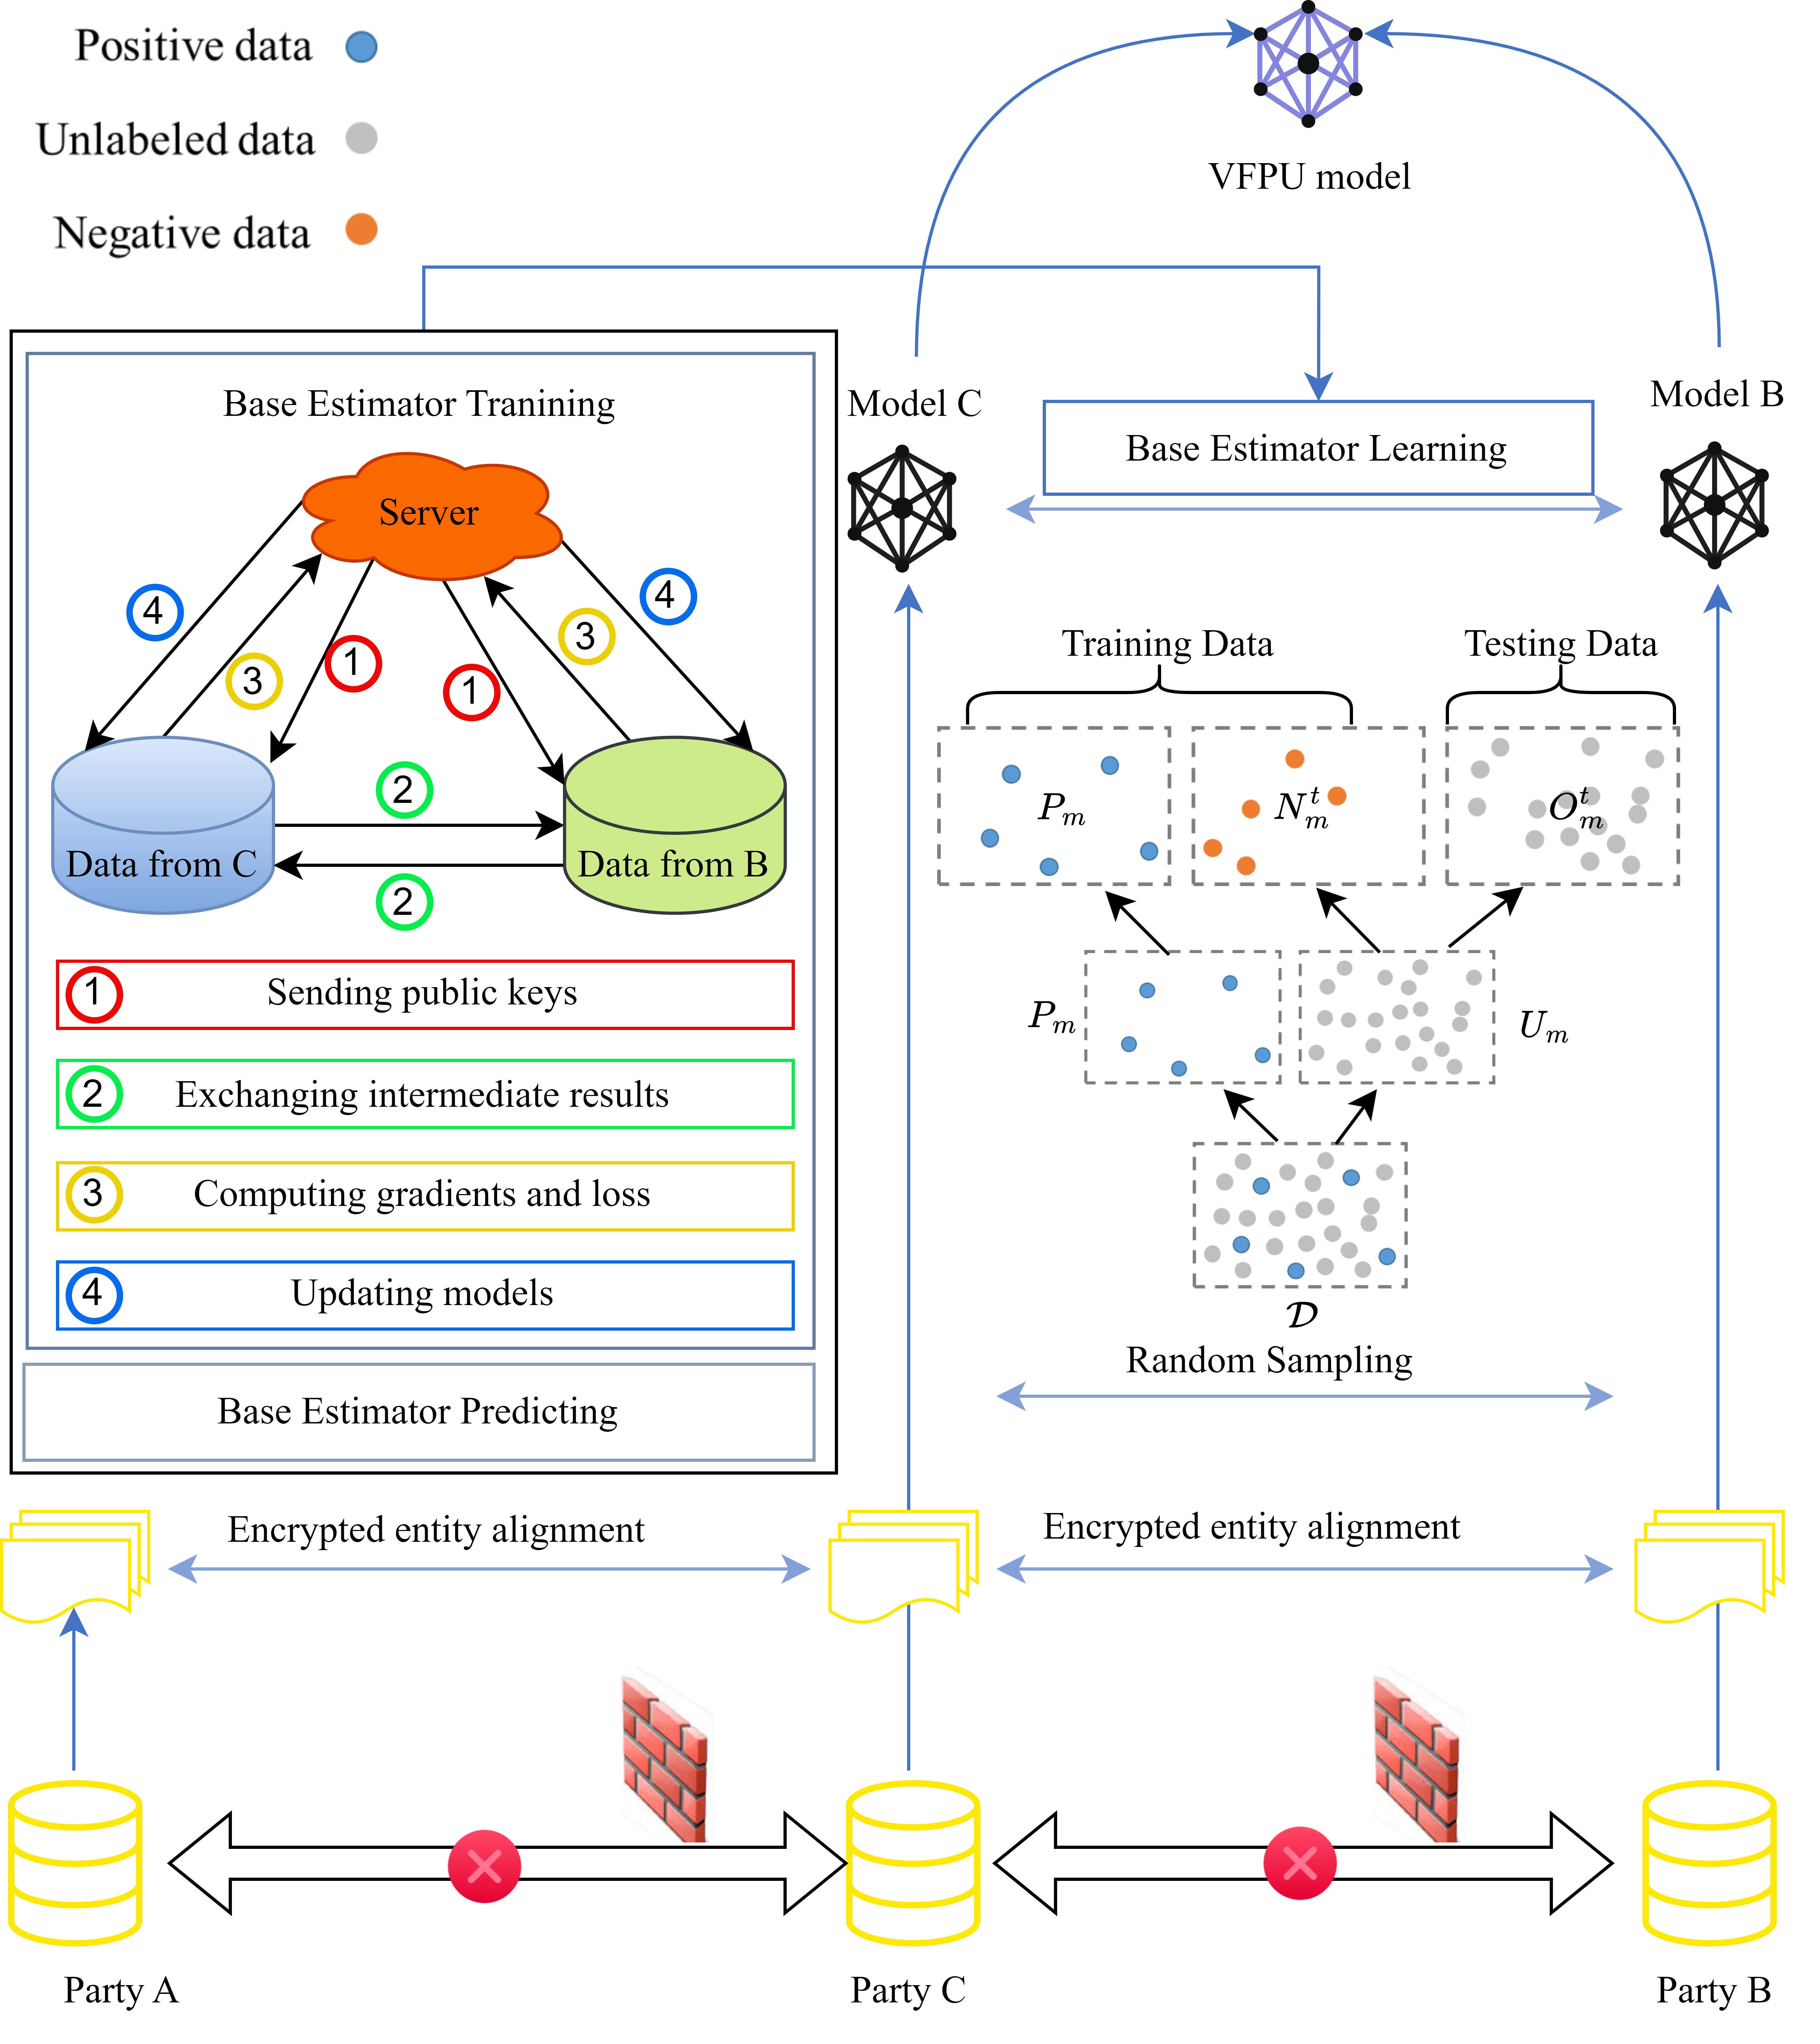
\includegraphics[width=0.9\textwidth]{chapters/imgs/Figure 1 in JEPG format}
	\bicaption[\xiaosi VFPU算法总体流程]
	{\wuhao VFPU算法总体流程}
	{\wuhao The overall process of the proposed VFPU algorithm}
	\label{fig:VFPU}
\end{figure}
\vspace{-0.35cm}
\subsection{数据预处理与加密样本对齐}
为了有效地训练模型,VFPU框架包含了一个两部分的预处理阶段:数据预处理和加密样本对齐。这些过程确保了来自A、B和C方的数据集在不损害隐私的情况下进行协调和安全对齐。 

(1) 数据预处理 

对A、B和C方持有的异构数据应用各种预处理技术,包括数据清洗、规范化和特征编码。数据清洗是第一步,它涉及解决常见的数据质量问题,例如通过插补或删除处理缺失值,消除重复项,并解决数据收集过程中可能出现的错误。这些努力确保数据集可靠,并且没有可能扭曲模型性能的噪声。规范化紧随其后,确保各方所有特征都达到可比的规模,这对许多机器学习算法的最佳运行至关重要。具体来说,数值特征使用标准化缩放进行规范化,这是一种将数据转换为零均值和单位方差的技术,从而防止范围较大的特征不成比例地影响模型。同时,分类特征通常表示定性属性,例如产品类别或用户人口统计信息,使用独热编码进行处理。此方法通过为每个类别创建二进制向量来将分类变量转换为数字格式,确保模型解释这些特征,而不假设从其他编码方案(如标签编码)可能产生的任何意外的序数关系。总之,这些预处理步骤创建了一个标准化、高质量的数据集,为后续处理做好准备。

(2) 加密样本对齐

在数据预处理之后,三方参与一个安全的样本对齐过程,该过程分两个不同的步骤进行,以同步其数据集,同时保护隐私。这种对齐对于实现纵向联邦学习至关重要,在纵向联邦学习中,不同的方持有重叠样本集的互补特征。 

步骤 1: B方和C方对齐其样本 ID 空间,只保留两方都共享的样本,丢弃未对齐的样本。此步骤确保B方和C方在一个共同的样本集上操作,这是纵向联邦学习的先决条件,在纵向联邦学习中,各方为相同的实体贡献不同的特征集,例如用户或项目。通过关注其样本集的交集,建立了一个一致的基础,其中B方和C方的特征对应于相同的人或项目,允许模型有效地从组合特征空间中学习。因此,B方和C方现在共享相同的样本,但保持独特的、互补的特征,为协作训练奠定了基础。

步骤 2: A方和C方对齐其样本 ID 空间,不删除任何样本,与步骤 1 相比采用了一种更具包容性的方法。对齐的样本定义为存在于A方和C方数据集中的样本,而未对齐的样本仅存在于C方。这种对齐过程利用了来自A方的可用标签信息来丰富C方的数据集。具体来说,出现在A方和C方中的样本在C方中被分配一个标签 1,表示它们是正样本,因为它们对应于A方数据中已知的正实例,例如与确认的产品交互的用户。相反,C方中缺少A方对应物的样本被分配一个标签 -1,将其标记为可能包含正负实例混合的未标记样本。这种标记策略将C方的数据集转换为适合 PU 学习的数据集,其中挑战在于区分未标记集中真正的正样本。通过不丢弃任何样本,此步骤最大限度地利用了可用于训练的数据,同时利用A方的正样本来指导该过程。

在完成加密样本对齐后,C方获得了一个包含正样本和无标签样本的数据集。这种转换有效地将原始的UDD-PU推荐问题——其特点是A方缺乏无标签数据——转变为一个纵向联邦训练场景。在这个场景中,PU学习问题由B方和C方协作解决,其中B方提供额外的特征,C方提供有标签和无标签的样本。这种合作框架充分利用了所有方的优势,克服了A方在数据方面的限制,最终使其推荐系统受益。

为了在样本对齐过程中保护数据隐私,采用了基于盲RSA的私有集交集(PSI)协议 \textsuperscript{\cite{de2010practical}}。这种密码学技术使所有方能够安全地计算其数据集的交集,而不会暴露除共享样本ID之外的任何信息。具体来说,PSI确保B方和C方能够识别它们的共同样本,同时A方和C方能够确定它们的重叠样本,而不会泄露各自数据集的全部内容或关于未对齐样本的任何敏感细节。这种保护隐私的机制是联邦学习范式的核心,促进了各方之间的信任,并确保遵守数据保护标准。随着数据预处理和加密样本对齐的顺利完成,B方和C方的数据集现已完全准备就绪——经过对齐、标记和保护——可以用于执行VFPU算法。该算法及其训练过程的细节将在后续章节中详细阐述,基于此处奠定的基础。


\subsection{基于正样本与未标记数据的纵向联邦学习}
纵向联邦PU学习(VFPU)算法的目标是在纵向划分的数据环境中,安全且高效地从未标记数据中识别可靠的正例样本。这种场景在现实应用中经常出现,其中不同的组织持有相同数据主体的不同特征,但由于隐私问题或法规限制,无法直接共享原始数据。例如,银行可能拥有金融交易记录,而电子商务平台则掌握在线购物历史,这些数据都与相同的客户相关。识别正例样本(如可能违约的贷款客户或可能响应特定营销活动的客户)至关重要,但由于缺乏完整的标注数据以及特征的分布式存储,这一任务极具挑战性。

VFPU 通过巧妙结合既有的正例与未标记(PU)学习技术和纵向联邦学习框架来应对这一挑战。具体而言,它利用了 Liu 等人\textsuperscript{\cite{liu2003building}} 提出的两步技术,以及 Mordelet 和 Vert \textsuperscript{\cite{mordelet2014bagging}} 提出的 PU bagging 方法的鲁棒性。这些方法经过调整和整合,形成了一种安全协议,使得各方能够在不泄露数据隐私的情况下进行协作训练。

算法 3-1 详细描述了 VFPU 过程。第一阶段采用两步技术,首先从未标记数据中识别出一组可靠的负例样本。这一过程利用了正例样本,并假设未标记数据中同时包含正例和负例。通过仔细分析特征分布,可以提取出可靠的负例集合,从而更准确地表示数据的真实分布。随后,利用这些可靠的负例样本以及原始的正例样本训练一个初步分类模型,该模型作为第二阶段的基础。


第二阶段引入 PU bagging 方法,以进一步增强 VFPU 的鲁棒性和性能。通过从正例和可靠负例集合中生成多个自助采样(bootstrap)样本,并在每个样本上训练独立的分类器,PU bagging 有效地缓解了初始可靠负例选择可能带来的偏差。最终预测结果通过集成这些独立分类器的预测结果获得,从而在未标记数据中更稳定、准确地识别正例样本。这种集成方法还增强了 VFPU 在处理噪声数据或不完整数据时的适应能力,而这些问题在现实数据集中普遍存在。

\vspace{-0.1cm} 
\begin{table}[h]
	\renewcommand{\arraystretch}{0.6}
	\centering
		{\songti \wuhao
			\begin{tabular}{p{\textwidth}}
				\toprule[1.5pt]
				\makecell[l]{\songti\wuhao 算法3-1 VFPU 算法训练过程}\\
				\midrule[0.75pt]
				\makecell[l]{\wuhao \textbf{输入:} 参与方 $B,C$。对齐的数据集 ${{\mathsf{\mathcal{D}}}_{B}}\text{,}{{\mathsf{\mathcal{D}}}_{C}}$ 和 ID 集合 ${{\mathsf{\mathcal{I}}}_{B}}\text{,}\ {{\mathsf{\mathcal{I}}}_{C}}$。}\\
				\makecell[l]{\wuhao \quad \ \ 最大迭代次数 $M$,随机采样迭代次数 $T$ 和采样率 $\theta$。}\\
				\makecell[l]{\wuhao \textbf{输出:} $R$,可靠正样本的集合。}\\
				\makecell[l]{\wuhao \textbf{参与方 C 执行:}}\\
				\makecell[l]{\wuhao 1: \ \textbf{for} $m=1,2,\ldots,M$ \textbf{do}}\\
				\makecell[l]{\wuhao 2: \quad ${{P}_{m}}=\{i|\mathsf{\mathcal{Y}}_{i}^{C}=1, \ i\in {{\mathsf{\mathcal{I}}}_{C}}\}$; ${{U}_{m}}=\{i|\mathsf{\mathcal{Y}}_{i}^{C}=-1, \ i\in {{\mathsf{\mathcal{I}}}_{C}}\}$}\\
				\makecell[l]{\wuhao 3: \quad \textbf{for} $t=1,2,\ldots,T$ \textbf{do}}\\
				\makecell[l]{\wuhao 4: \qquad $N_{m}^{t}=\{从 {{U}_{m}} 中随机选择 |{{P}_{m}}| 个元素\}$; $O_{m}^{t}={{U}_{m}}-N_{m}^{t}$}\\
				\makecell[l]{\wuhao 5: \qquad 加密并发送 $N_{m}^{t}$、${P_m}$ 和 $O_{m}^{t}$ 给其他参与方;通知设置训练和测试数据。}\\
				\makecell[l]{\wuhao 6: \qquad $S_m^t$ = Base\_Estimator\_Learning()}\\
				\makecell[l]{\wuhao 7: \quad \textbf{end for}}\\
				\makecell[l]{\wuhao 8: \quad ${{\mathsf{\mathcal{P}}}_{m}}(u)={\sum\nolimits_{t=1}^{T}{S_{m}^{t}}}(u)/{\sum\nolimits_{t=1}^{T}{I(u\in O_{m}^{t})\text{,}\ \ \forall \text{u}\in }}\;{{U}_{m}}$}\\
				\makecell[l]{\wuhao 9: \quad ${{R}_{m}}=\{从 {{\mathsf{\mathcal{P}}}_{m}} 中选择前 |{{U}_{m}}| \times \theta 个 ID\}$; $\mathsf{\mathcal{Y}}_{r}^{C}=1\text{,}\ \ \forall r\in {{R}_{m}}$}\\
				\makecell[l]{\wuhao 10: \textbf{end for}}\\
				\makecell[l]{\wuhao 11: $R=\bigcup\limits_{m=1}^{M}{{{R}_{m}}}$}\\
%				\midrule[0.5pt]
				\makecell[l]{\wuhao \textbf{函数} Base\_Estimator\_Learning():}\\
				\makecell[l]{\wuhao 12: 服务器创建加密密钥对,将公钥发送给 $B$ 和 $C$}\\
				\makecell[l]{\wuhao 13: $B$ 和 $C$ 加密、交换梯度和损失,添加掩码,将加密值发送给服务器。}\\
				\makecell[l]{\wuhao 14: 服务器解密并回传值。$B$ 和 $C$ 去除掩码,更新模型。}\\
				\makecell[l]{\wuhao 15: \textbf{返回:} 测试数据上正类的预测概率。}\\
				\bottomrule[1.5pt]
			\end{tabular}
		}
	\label{tab:algo-vfpu} 
\end{table}
\vspace{-0.35cm}

此外,纵向联邦学习框架确保了整个过程中的数据隐私。每个参与方都保留对自身数据的控制权,并且在训练过程中仅共享中间结果(如模型参数或加密梯度)。这种去中心化的方法避免了集中式数据存储的需求,并最大程度地降低了数据泄露的风险。VFPU 结合了强大的 PU 学习技术和纵向联邦学习的隐私保护特性,为分布式环境下涉及正例和未标记数据的各种现实应用提供了一种有前景的解决方案。这一方法为更高效的协作和知识发现铺平了道路,同时遵守数据隐私标准。

(1) 建立初始样本集

VFPU 算法采用迭代方式运行,并通过双层方法增强正样本识别过程的稳健性和可靠性。外层循环包含 $M$ 次迭代,为优化可靠正样本的选择提供了多次机会。在每次迭代 $m \in \{1, ..., M\}$ 中,内层循环执行 $T$ 轮随机采样、训练和预测。这种嵌套结构有助于提高算法的稳定性和准确性,尤其是在处理现实场景中常见的噪声数据或不平衡数据时。

在每次迭代 $m$ 开始时,算法基于 C 方提供的标签建立两个基本样本集。在纵向联邦学习框架中,C 方被指定为持有训练数据标签或部分标签的一方。这一指定至关重要,因为它指导了数据的初始划分。这两个集合定义如下:
\begin{equation}
	\begin{split}
		&{{P}_{m}}=\{i|\mathsf{\mathcal{Y}}_{i}^{C}=1,\ i\in {{\mathsf{\mathcal{I}}}_{C}}\};\\
		&{{U}_{m}}=\{i|\mathsf{\mathcal{Y}}_{i}^{C}=-1,\ i\in {{\mathsf{\mathcal{I}}}_{C}}\},
	\end{split}
\end{equation}

式中,${{\mathsf{\mathcal{I}}}_{C}}$ 表示 C 方的 ID 空间,即 C 方可用的所有样本标识符的集合。${{\mathsf{\mathcal{Y}}}^{C}}$ 表示 C 方的标签空间,包含每个样本 ID 对应的标签。$i$ 代表 ID 空间中的特定样本 ID。因此,${{P}_{m}}$ 代表迭代 $m$ 中的正样本集,具体而言,即 C 方提供正标签($\mathsf{\mathcal{Y}}_{i}^{C}=1$)的样本集合。相反,${{U}_{m}}$ 代表迭代 $m$ 中的未标记样本集,包含 C 方提供负标签或未标记($\mathsf{\mathcal{Y}}_{i}^{C}=-1$)的样本。

需要注意的是,在 PU 学习(Positive-Unlabeled Learning)的背景下,未标记集合 ${{U}_{m}}$ 假设包含真实的正样本和真实的负样本的混合体。VFPU 旨在有效地区分这些样本,并在 ${{U}_{m}}$ 中识别出可靠的正样本。该算法的迭代特性,以及后续涉及 PU 学习技术的步骤,有助于完成这一去歧义过程。通过在多个迭代和采样轮次中不断优化正样本的选择,VFPU 旨在逐步收敛到更准确、更稳健的真实正样本识别结果。这种精细的划分和迭代优化对于在未标记数据的情况下实现高性能至关重要。

(2) 采样、训练与预测

如图 \ref{fig:VFPU} 所示,在第 $m$ 次迭代的第 $t\text{-th} \ (\text{t}\in \{1,2,...,T\})$ 轮采样过程中,使用自助法(bootstrapping)\textsuperscript{\cite{mordelet2014bagging}} 从 $U_{m}$ 生成伪负样本集 $N_{m}^{t}$。数学上可以表示为:
\begin{equation}
	N_{m}^{t}=\{ \text{Randomly select} \ |P_{m}| \ \text{elements from} \ U_{m} \},
\end{equation}
式中,$|P_{m}|$ 是 $P_{m}$ 中包含的样本数量。在此过程中,随机选择是有放回的,这意味着 $U_{m}$ 中的同一元素可能会被多次选中。这种策略不仅在样本生成过程中引入了随机性,还在不确定 $U_{m}$ 内真实标签分布的情况下,有助于构建一个平衡的数据集。

由于未标记样本的实际类别未知,$N_{m}^{t}$ 被视为一组伪负样本,可能同时包含真正的负样本和正样本。通过从 $U_{m}$ 中抽取 $|P_{m}|$ 个元素,可以构造出与 $P_{m}$ 规模相同的 $N_{m}^{t}$,从而为分类任务提供一个可比且平衡的数据集。这种平衡对于机器学习至关重要,因为它试图减轻类别不平衡可能带来的不利影响,并为后续的训练过程提供一个稳健的样本空间。

在训练过程中,$P_{m}$ 和 $N_{m}^{t}$ 被合并为一个二元分类训练集。该训练集用于训练纵向联邦学习模型,使其能够区分正样本和负样本,并将此知识应用于未来的预测任务。这两个集合的结合确保了学习算法能够接触到多样化的示例,在优化训练模型的泛化性能方面发挥着至关重要的作用。此外,训练过程同时利用了真实的正样本和伪负样本,即使伪负样本集中可能包含被错误标记的数据点,也能促进模型学习到稳健的决策边界。

自助法(bootstrapping)是一种从数据集中随机选择样本(有放回)的技术。这种统计方法在机器学习中被广泛采用,因为它有助于减少过拟合,并提供对模型性能更精确的估计。采用该技术使 VFPU 能够创建多样化且平衡的训练集,从而提高模型的泛化能力,减少潜在偏差,并增强推荐模型的整体性能。此外,在难以获取真实负样本的情况下,该方法尤为有用,因为它通过合成一个近似于真实负样本分布的伪负样本集,弥补了标注数据不足的问题。

在自助法过程中未被选中的样本称为袋外样本(out-of-bag samples)。这些样本在验证模型性能方面发挥着重要作用,因为它们提供了对分类误差的无偏估计。袋外评分(out-of-bag score)表示袋外样本被分类为正样本的预测概率。因此,为了获得袋外样本集 $O_{m}^{t}$,需要从 $U_{m}$ 中排除 $N_{m}^{t}$ 中的样本,数学表达如下:
\begin{equation}
	O_{m}^{t}=U_{m}-N_{m}^{t}.
\end{equation}

这种策略提供了一种内部模型评估机制,而无需单独划分验证集,从而充分利用所有可用数据进行模型开发和性能估计。

然后,C 方对 $N_{m}^{t}$、$P_{m}$ 和 $O_{m}^{t}$ 进行加密,并将其发送给其他方。在示例中,另一方是 B 方。随后,B 方和 C 方基于交换的三组样本 ID 共同建立各自的训练和测试数据集。这一联合过程在联邦学习环境中至关重要,因为隐私和数据安全是首要考虑因素。具体来说,按照以下公式进行数据集构建:
\begin{equation}
	\begin{split}
		&\mathsf{\mathcal{D}}_{train}^{K}=\{(i,x_{i},y_{i}) \ | \ i\in P_{m}\ or\ i\in N_{m}^{t}\};\\
		&\mathsf{\mathcal{D}}_{test}^{K}=\{(i,x_{i},y_{i}) \ | \ i\in O_{m}^{t}\},
	\end{split}
\end{equation}

式中,$\mathsf{\mathcal{D}}_{train}^{K}$ 代表二元分类训练数据,$\mathsf{\mathcal{D}}_{test}^{K}$ 代表测试数据,$K\in \{B,C\}$。这里,$x_{i}\in \mathsf{\mathcal{X}}$ 表示样本 $i$ 关联的特征向量来自特征空间 $\mathsf{\mathcal{X}}$,而 $y_{i}\in \mathsf{\mathcal{Y}}$ 表示相应的标签属于标签空间 $\mathsf{\mathcal{Y}}$。这种加密样本 ID 与相应特征的无缝集成,促进了一个安全且协作的训练环境,在需要高隐私标准的场景中至关重要,同时确保了高质量的模型输出。

总之,通过结合自助法、袋外评估机制以及联邦学习方之间的安全样本共享机制,方法有效应对了处理不平衡和部分标注数据集的常见挑战。这种方法不仅保证了多样化的训练过程,还显著增强了模型在实际应用中的预测结果的完整性和可靠性。

一旦B方和C方准备好了各自的训练和测试数据集,二分类问题就转变为一个纵向联邦训练和预测任务。在这种情况下,一个基学习器——代表每个参与实体的传统机器学习模型——被调整为可在纵向联邦学习(VFL)框架内使用,理解VFL的一般训练过程至关重要。总体而言,这个过程包括四个关键步骤,这些步骤共同展示了如何在多方训练数据上训练基学习器,同时确保在整个合作过程中严格保护各方数据集的隐私\textsuperscript{\cite{yang2019federated}}。四个步骤的描述如下:

(1)服务器通过生成一系列加密密钥对来启动该过程。在此过程中,服务器安全地创建这些加密材料,并将相应的公钥发送给B方和C方。这一步为后续的所有隐私保护操作奠定了基础,建立了一个安全的信息交换通道。

(2)在收到公钥后,B方和C方对中间计算结果进行加密并交换这些结果。这些结果至关重要,因为它们涉及到梯度和损失的计算,这些计算对于学习过程至关重要。通过仅共享加密数据,每方确保不会直接透露或传输原始的敏感数据值,从而遵守了VFL范式中固有的隐私约束。

(3)在交换加密的中间结果后,B方和C方计算必要的加密梯度,用于模型参数的更新。除了计算这些梯度外,双方还引入了额外的掩码机制,以进一步隐藏计算出的梯度值。同时,每方还计算了加密版本的模型损失。应用这一额外的掩码步骤是为了防止在后续传输过程中可能发生的数据泄露。一旦这些涉及梯度和损失的加密值生成,它们会被安全地传输到服务器进行进一步处理。

(4)在收到加密数据后,服务器负责解密接收到的梯度和损失。在完成解密过程后,服务器将解密后的梯度和损失发送回B方和C方。收到后,双方将移除之前应用的额外掩码。这个去掩码步骤至关重要,因为它恢复了真实的梯度信息,这对于更新模型参数是必需的。只有在这些梯度成功去掩码后,B方和C方才会对基学习器执行实际的参数更新,从而以同步和隐私保护的方式推进训练过程。

为了支持在VFL框架内的一般训练过程,已提出多种隐私保护的机器学习算法\textsuperscript{\cite{yang2019federated}}。其中一些著名的例子包括逻辑回归(LR)\textsuperscript{\cite{he2021secure,yang2019parallel}}、随机森林(RF)\textsuperscript{\cite{yao2022efficient}}、梯度提升决策树(GBDT)\textsuperscript{\cite{he2021secure}}、XGBoost(XGB)\textsuperscript{\cite{xu2021efficient,wang2022feverless}}和LightGBM(LGB)\textsuperscript{\cite{feng2019securegbm}}。这些算法旨在促进安全和高效的训练,同时在多个数据所有者之间保持数据隐私。在本文中,利用不同的基学习器——每个算法对应其中之一——来全面评估推荐模型的整体性能。这种多估计器评估不仅突显了VFL框架的灵活性和广泛适用性,还提供了关于不同模型在隐私保护设置下行为的深入见解。包含多种模型架构强化了方法在处理复杂且敏感数据集时的鲁棒性和适应性,适用于跨不同数据源的应用。

通过仔细遵循上述四个步骤,并结合成熟的隐私保护技术,所提出的方法确保了模型性能与数据安全之间的强平衡。加密数据的交换、协作计算以及随后的解密和去掩码过程,展示了防止任何无意暴露敏感信息的严格措施。因此,这一过程促进了一个安全的训练环境,各方可以共同从集体数据洞察中受益,同时严格遵守隐私协议,使其特别适用于涉及敏感或受监管数据的应用。 

(3) 确定可靠正样本

在第 $m\text{-th}$ 次迭代中,采样、训练和预测的整体过程被重复执行 $T$ 轮。完成这 $T$ 轮后,会积累大量信息,从而形成一组概率,记为 ${{\mathsf{\mathcal{P}}}_{m}}$,它与 ${{U}_{m}}$ 中所有未标记样本相关联。这些概率反映了 ${{U}_{m}}$ 中每个样本属于正类的可能性或置信度。这些概率评分在后续决策过程中起着关键作用,例如识别一部分高度可靠的正样本,并迭代更新训练集以提升模型性能。

为了计算完整的集合 ${{\mathsf{\mathcal{P}}}_{m}}$,有必要为每个未标记样本 $u$(其中 $u\in {{U}_{m}}$)确定概率 ${{\mathsf{\mathcal{P}}}_{m}}(u)$。该概率 ${{\mathsf{\mathcal{P}}}_{m}}(u)$ 是通过将样本 $u$ 在第 $m\text{-th}$ 次迭代中所有 $T$ 轮的袋外评分相加,然后除以 $u$ 在这些轮中作为袋外样本出现的总次数来归一化得到的。该过程在数学上可表示为以下公式:
\begin{equation}
	{{\mathsf{\mathcal{P}}}_{m}}(u)=\frac{\sum\nolimits_{t=1}^{T}{S_{m}^{t}}(u)}{\sum\nolimits_{t=1}^{T}{I(u\in O_{m}^{t})}}.
\end{equation}
在该表达式中,$S_{m}^{t}(u)$ 表示在第 $m\text{-th}$ 次迭代中第 $t\text{-th}$ 轮为样本 $u$ 分配的袋外评分。值得注意的是,如果 $u$ 在某一轮中未作为袋外样本出现,则定义 $S_{m}^{t}(u)$ 为 0。指示函数 $I(u\in O_{m}^{t})$ 在样本 $u$ 包含在袋外集合 $O_{m}^{t}$ 中时取值为 1,否则取值为 0。因此,分母 $\sum\nolimits_{t=1}^{T}{I(u\in O_{m}^{t})}$ 有效地计数了 $u$ 参与袋外估计的轮数。此归一化过程确保分配给每个样本的概率反映了其在参与预测的各轮中的平均表现,从而提高了所得概率估计的鲁棒性和可靠性。

基于计算得到的概率 ${{\mathsf{\mathcal{P}}}_{m}}(u)$,接下来对 ${{U}_{m}}$ 中的所有未标记样本进行排序。该排序以非递增顺序执行,因此具有较高概率的样本(即更可能为真正正样本的样本)会排在列表的顶部。利用这一排序好的列表,下一步便是选择一组可靠正样本。正式地,令 ${{R}_{m}}$ 表示在第 $m\text{-th}$ 次迭代中识别出的可靠正样本集合。在方法中,通过选择排名前 $|{{U}_{m}}|\times \theta$ 的样本来进行选择,式中 $\theta$ 是手动设置的比例,代表可靠正样本的采样率。该选择过程可简洁地表述为:
\begin{equation}
	{{R}_{m}}=\{Chose\ Top\ |{{U}_{m}}|\times \theta \ IDs\ from\ {{\mathsf{\mathcal{P}}}_{m}}\}.
\end{equation}
这一两步选择过程可以具体描述为:
\begin{itemize}
	\item 第一步:将 ${{\mathsf{\mathcal{P}}}_{m}}$ 中的所有样本按照计算得到的概率以非递增顺序进行排序。此排序确保最有可能为正样本的样本获得优先考虑。
	
	\item 第二步:从排序结果中选择前 $|{{U}_{m}}|\times \theta$ 个样本,式中 $\theta$ 作为可调参数决定了未标记数据集中被视为可靠正样本的样本比例。
\end{itemize}
通过执行这一过程,最有信心且可能真正属于正类的样本便从其他样本中被区分出来。因此,集合 ${{R}_{m}}$ 包含了这些被选中的样本,并随后被用来更新由 Party C 维护的训练标签。

在识别过程之后,这些新识别出的可靠正样本会被纳入 Party C 维护的训练集中。此更新过程包括为 ${{R}_{m}}$ 中的每个样本分配一个正标签,从而逐步减少未标记数据集 ${{U}_{m}}$ 的规模。从形式上表示,该更新过程表达为:
\begin{equation}
	\mathsf{\mathcal{Y}}_{r}^{C}=1,\ \ r\in {{R}_{m}},
\end{equation}
式中,集合 ${{R}_{m}}$ 中的每个样本 $r$ 被明确赋予标签 1,表明其被归类为正类。该标签更新在训练数据的迭代细化过程中至关重要,因为它利用了从袋外预测集合中获得的置信度评分来提高后续迭代中训练集的整体质量和可靠性。

总之,识别可靠正样本的过程是一种精心设计的机制,它将概率预测转换为一组高置信度的正实例。该机制不仅提升了训练数据的质量,还为改进整体推荐模型性能提供了一个迭代途径。通过基于样本的袋外表现不断更新样本标签,算法有效地缓解了标签不确定性和数据稀疏性相关的问题。此外,这种丰富而系统的方法为后续的模型训练和预测任务奠定了坚实的基础,确保不断发展的数据集逐步趋向更高的准确性和一致性。 

(4) 最终结果及其在推荐中的应用

完成算法的所有 $M$ 次迭代后,最终的可靠正样本集合 $R$ 是通过取每次迭代中所有 ${{R}_{m}}$ 集合的并集得到的,其中 $m = 1, 2, \dots, M$ 表示在整个过程中所执行的各个单独迭代。该迭代方法确保算法在多个轮次中系统地细化正样本的选择,逐步提升最终集合 $R$ 的质量和可靠性。具体来说,每个 ${{R}_{m}}$ 包含在第 $m$ 次迭代中识别出的正样本,而并集操作则将这些中间结果整合为一个全面的最终集合。该步骤在计算上虽简单但至关重要,因为它将所有迭代的结果聚合成一个统一的集合,反映出算法在从整个数据集中区分可靠正样本方面所做的累计努力。

借助这一精心筛选出的可靠正样本集合 $R$,Party A(可能代表服务提供商或推荐系统运营者等相关方)现在可以利用这些信息为 $R$ 中的每个样本量身定制推荐。该个性化过程涉及对每个样本的特征或偏好进行分析,并设计与之匹配的推荐策略。通过这种方式,Party A 能显著提高推荐系统的准确性和相关性,确保向最终用户提供的建议——无论是产品推荐、内容建议还是其他个性化输出——既精准又符合情境。基于一组可靠正样本对推荐进行微调的能力,凸显了该算法的实际效用,将理论计算与实际应用相结合。

利用 $R$ 来增强推荐系统的这一步骤不仅仅是一个程序上的形式问题,而是整个算法有效性的基石。推荐系统的成功取决于其识别和优先考虑最相关样本的能力,而这一任务正是该迭代算法通过其结构化设计所完成的。通过聚焦于可靠正样本,系统最大程度地减少了噪声或无关数据的引入,这些数据本可能降低推荐质量。此外,$R$ 的应用使得 Party A 能够优化资源分配——将计算和操作上的努力集中在最有可能带来高用户满意度和参与度的样本上。

为说明这一过程的重要性,可以考虑推荐系统在各个领域的广泛应用,如电子商务平台、流媒体服务和社交网络,其中建议的准确性直接影响用户体验和业务成果。通过取 ${{R}_{m}}$ 集合的并集来创建 $R$,确保了这些应用的坚实基础,提供了一种可扩展且适应性强的解决方案,能够容纳不同规模和复杂度的数据集。此外,算法的迭代特性使其能够适应用户偏好或数据分布可能随时间变化的动态环境,从而成为长期部署的多功能工具。

在实践中,可以通过精确度、召回率或用户满意度等指标来评估这一最终步骤的有效性,这些指标量化了由于精心筛选出的集合 $R$ 而提升的推荐质量。例如,更高的精确度表明推荐项中相关的比例更大,而召回率的提升则反映了系统从数据集中检索出更广泛相关项的能力。这些可衡量的结果突显了算法在提升推荐系统性能方面所作的贡献,验证了迭代过程及随后 $R$ 应用的重要性。因此,这一收尾阶段不仅完成了算法工作流程,也确立了其作为解决现实推荐挑战的实际方案的价值。  

\section{实验过程及结果分析}
本节描述了 VFPU 算法的实验设计和评估。首先,提供了数据集和实验设置的概述。随后,提出了一组用于指导实验的研究问题,然后根据每个研究问题展示并讨论实验结果。
\subsection{数据集介绍与实验准备}
在实验中,利用了三个多样且成熟的数据集来评估所提出方法的有效性:Bank Marketing Datasetg\textsuperscript{\cite{fitriani2021data}}、Default of Credit Card Clients Dataset\textsuperscript{\cite{subasi2019prediction}} 以及 Adult Census Dataset\textsuperscript{\cite{chakrabarty2018statistical}}。每个数据集的选择都经过精心考虑,以代表不同的真实世界领域和预测挑战,从而使能够在多样化的场景下对方法的鲁棒性进行评估。

Bank Marketing Dataset 源自 UCI 机器学习库,数据来自葡萄牙某银行针对定期存款产品进行的直销电话营销活动。这些活动通过电话直接与客户沟通,旨在说服他们订购定期存款产品。完整的数据集包含四个版本,但在本研究中,专门采用了“bank-additional-full”版本,该版本包含 41,188 个样本和 20 个输入特征。这些特征涵盖了客户的各种属性,包括年龄、工作类型、婚姻状况、教育程度以及诸如是否有住房贷款或个人贷款等金融细节,同时也包括了营销活动相关变量,如联系次数和以往互动的结果。数据按照日期顺序排列,涵盖了从 2008 年 5 月到 2010 年 11 月的时间段,反映了此期间营销工作的时间演变。该数据集的主要分类目标是预测客户是否会订购定期存款,由变量“y”(是/否)表示的二元结果。此数据集在客户关系管理方面具有实际意义,并且由于大多数客户并未订购,从而带来了类别不平衡的问题,这为预测建模带来了实际挑战。

Default of Credit Card Clients Dataset 来自 Kaggle,提供了30,000 名信用卡客户财务行为的详尽数据,数据集中包含 24 个变量。这些变量融合了丰富的人口统计信息(如性别、教育、婚姻状况和年龄)和详细的还款历史数据,涵盖了每月账单、前期还款金额以及多个月份内的付款延迟记录。该数据集为构建预测模型以评估客户下月违约风险提供了基础,其目标变量为表示违约状态(是/否)的二元指标。人口统计和交易特征的结合为信用风险提供了细致的视角,使该数据集在金融分析中极具价值。其庞大的数据量和详细的特征集进一步提升了其在训练和评估旨在信用风险预测的复杂机器学习模型中的适用性。

Adult Census Dataset 同样源自 UCI 机器学习库,是一个广泛认可的人口统计和社会经济数据集,数据来自 1994 年美国人口普查。该数据集包含各种属性,如年龄、工作类别(例如私人部门、联邦政府)、教育程度、职业、种族、性别、资本利得、资本损失、每周工作小时数以及原籍国,为个人特征提供了详尽的快照。数据集的分类任务是预测个人年收入是否超过 50,000 美元,这一二元结果已成为收入预测模型的基准。除了在机器学习中的应用之外,该数据集还经常被研究人员和从业者用于探讨与收入分配、就业趋势和经济差异相关的社会模式。其多样的特征集和现实意义使其成为评估预测模型的理想候选者,同时也应对了诸如缺失值和类别数据处理等挑战。为简洁起见并在本文中保持一致性,分别将这些数据集称为“Bank”、“Credit”和“Census”。

在数据预处理阶段,采用了系统化技术以确保数据集适用于机器学习算法。所有三个数据集中普遍存在的分类特征(例如“Bank”中的工作类型、“Credit”中的教育程度以及“Census”中的职业)均采用独热编码(one-hot encoding)进行编码。该方法将分类变量转换为一系列二元列,每个列对应一个类别,从而防止模型错误地假设类别之间存在序数关系,并能有效地进行数值处理。数值特征,如年龄或账单金额,则使用标准化缩放方法进行归一化,该方法将数据中心化为均值为零并缩放为单位方差。这种归一化确保了不同尺度的特征在模型学习过程中具有同等的贡献,尤其对于依赖梯度优化的算法尤为关键。

各数据集均由各自数据提供方预先划分为训练集和测试集,确保模型训练与在未见数据上的评估有初步的分离。为了与实验设计保持一致,该设计模拟了分布式学习环境,进一步将训练数据纵向划分为三个不同部分,分别分配给三个假想方:A、B 和 C。该纵向划分意味着每个方持有整个样本集中的一部分独特特征,这反映了数据在多个实体间分布的场景,正如联邦学习框架中常见的情况。为模拟标签数据稀缺或分布不均的情况,从方 B 和 C 持有的数据中移除了数据标签,从而生成了统称为 U 的未标记数据。对于方 A,在其训练数据子集中识别出所有属于正类的样本,并随机选择其中 10\% 的样本保留其标签,构成正样本集 P。而对于其余 90\% 的正样本以及所有负样本,其标签均被忽略,在方 A 的数据中这些样本实际上被视为未标记。因此,实验设置由仅供方 A 使用的一小部分标记正样本集 P,以及分布于三个方的更大未标记数据集 U 组成,从而使能够探讨方法在分布式环境下利用有限标记数据的能力。

在纵向联邦预测不确定性(VFPU)算法的联邦训练和预测阶段,通过集成针对纵向联邦学习(VFL)场景量身定制的多样化基学习器,对其性能进行了严格评估。具体而言,纵向联邦逻辑回归(VFPU\_LR)的实现改编自 Aono 等人的基础性工作 \textsuperscript{\cite{aono2016scalable}},该工作利用安全多方计算(SMC)协议在梯度交换过程中保护数据隐私。对于基于树的方法,则使用 FedTree 库 \textsuperscript{\cite{li2022fedtree}} 开发了纵向联邦梯度提升决策树(VFPU\_GBDT)和纵向联邦随机森林(VFPU\_RF),该库是一个针对分布式树构建并支持同态加密的最先进框架。此外,纵向联邦 LightGBM(VFPU\_LGB)的实现则基于 FATE(Federated AI Technology Enabler)框架 \textsuperscript{\cite{liu2021fate}},该框架为跨异构数据分区的安全联邦模型训练和推断提供了强大的基础设施。  

为建立全面的基准对比体系,研究采用传统集中式机器学习范式,在聚合数据集上训练了多种经典模型以模拟非联邦学习场景。具体涵盖逻辑回归(LR)、梯度提升决策树(GBDT)、随机森林(RF)等基于scikit-learn框架\textsuperscript{\cite{pedregosa2011scikit}}的模型,以及通过原生库实现的XGBoost(XGB)\textsuperscript{\cite{chen2015xgboost}}和LightGBM(LGB)\textsuperscript{\cite{ke2017lightgbm}}两类高性能集成算法。通过与联邦学习框架进行横向对比,揭示了两者在数据分散场景下的性能差异与适用边界。


实验中统一了超参数配置以确保公平性。为平衡计算效率与模型收敛性,最大迭代次数 $ M $ 固定为 5,而特征采样率 $ \theta $ 被设置为 0.02,以缓解高维数据场景中的过拟合问题。为确保随机优化的稳定性,随机采样迭代次数 $ T $ 设定为 10。针对 VFL 中固有的数据隐私问题,在跨方计算中采用了密钥长度为 512 位的 Paillier 加密系统 \textsuperscript{\cite{paillier1999public}} 对中间输出进行加密。此密钥长度在加密安全性与计算开销之间提供了务实的折衷。所有实验均假定默认的两方设置 \textsuperscript{\cite{li2022fedtree}},反映了现实中拥有互补特征空间的组织间常见的 VFL 协作模式。  

评估指标:  
采用了多维度评估框架以全面评估模型性能。准确率(acc)和 F 分数(F)\textsuperscript{\cite{cheng2021secureboost}} 分别量化了整体预测正确性和类别特定的平衡性。精确率和召回率 \textsuperscript{\cite{liu2003building}} 被用来评估第一类/第二类错误的权衡,这在不平衡分类任务中尤为关键。ROC 曲线下面积(AUC)\textsuperscript{\cite{cheng2021secureboost}} 提供了一个与阈值无关的正负类别可分性度量。  

AUC 指标来源于接收器操作特征(ROC)曲线,对于在不同决策阈值下评估模型鲁棒性尤其具有信息量,因为它量化了所有分类阈值下真正率(灵敏度)与假正率(1-特异性)之间的关系。与此同时,F 分数被定义为精确率与召回率的调和平均值,在类别分布偏斜或误分类成本不对称的场景下,作为模型稳定性的统一指标。这些指标均通过 5 折交叉验证在独立测试集上计算,以确保统计可靠性。  
\subsection{实验设计与基线模型介绍}

实验一:比较联邦和非联邦的 PU 学习的性能,在本实验设计中,深入研究了联邦学习对正类和无标签(PU)学习性能的影响。具体来说,比较了使用VFPU算法的联邦PU学习与非联邦PU学习在多种基学习器和数据集上的表现。核心目标是评估在其他算法参数和实验配置保持不变的情况下,联邦学习对分类质量的影响程度。

使用了四种常用的基学习器——逻辑回归(LR)、随机森林(RF)、梯度提升决策树(GBDT)和LightGBM(LGB)——在三个真实世界的数据集上进行实验:银行营销数据集、信用卡客户违约数据集和成人普查数据集。对于逻辑回归(LR),使用了L2惩罚系数为0.8、学习率为0.001、批处理大小为64的配置,确保在联邦和非联邦运行中收敛行为保持一致。对于基于决策树的算法(RF、GBDT和LGB),将树的数量设置为50,最大深度为6,学习率为0.1。这些设置经过精心选择,以平衡模型复杂度、训练时间和泛化能力。

实验二:分析不同基学习器对 VFPU 性能的影响,在这一部分,对集成在VFPU框架中的不同基估计器进行了深入评估,这些估计器包括VFPU\_LR、VFPU\_GBDT、VFPU\_RF和VFPU\_LGB,它们被用于解决UDD-PU问题。为了全面评估它们的性能,进行了一系列实验,重点关注四个关键评估指标:精确度(Precision)、召回率(Recall)、F-score以及精确度-召回率曲线。本次评估的主要目标是分析这些指标随着可靠正样本数量增加的变化趋势,并根据这些观察到的趋势,确定方法的最佳基估计器。

在实验中,采用随机抽样策略从一个未标记的数据集中选择可靠的正样本子集。这种方法不仅模拟了现实情况下可能已知少量正实例的条件,还严格测试了每个基估计器在利用这些有限样本时的鲁棒性。实验结果详见图 \ref{RQ2.1} 至 图 \ref{RQ2.3}。

对于基于逻辑回归(LR)的算法,配置了以下特定超参数:应用了L2惩罚,系数设置为0.8,学习率为0.001,小批量大小为64。这些参数基于初步实验精心选择,以确保收敛速度和模型泛化能力之间的平衡。另一方面,对于所有基于树的算法——即梯度提升决策树(GBDT)、随机森林(RF)和LightGBM(LGB)——将树的数量设置为50,树深限制为6以避免过拟合,并使用0.1的学习率。这种在三个数据集上的统一设置,使得在一致的实验条件下公平比较它们的性能成为可能。

实验三:基线对比实验,在本实验设计中,对所提出的针对UDD-PU问题的方法进行了全面探讨,特别是在纵向联邦学习(VFL)的设定下,为评估该方法的有效性设计了严谨的分析。为此,开展了两个不同的实验。第一个实验旨在识别最有效的解决正-未标记(PU)问题的半监督学习方法。这些方法虽广泛应用于UDD-PU问题的研究,但通常是在非联邦环境下考虑。第二个实验则基于第一个实验的结果,将前四种半监督技术在实现UDD-PU问题的VFL环境中进行比较。

在第一个实验中,对比了No\_Fed\_VFPU\_GBDT方法与另外九种在非联邦环境下运行的知名半监督学习方法。该对比结果在表 \ref{RQ3.1} 中进行了全面展示。以下段落进一步介绍了每种方法的背景及其在本研究中的具体实现细节。

\begin{quote}
	\textbf{\_GBDT:} 此方法涉及直接将梯度提升决策树(GBDT)分类器应用于正-未标记(PU)数据集。在这种方法中,未标记的数据(记为U)被当作负样本,而现有的标记数据(P)被视为正样本。这一基线方法为评估在没有特殊处理隐藏正样本的情况下,传统技术在PU学习中所面临的内在挑战提供了参考。
\end{quote}

\begin{quote}
	\textbf{Bagging\_GBDT:} Bagging\_GBDT代表了一种利用装袋(bagging)技术进行PU学习的集成学习方法。在这种方法中,通过对未标记数据集的反复采样生成多个训练集。每个训练集都包含正样本和未标记样本的混合,从而生成一系列多样化的子集,并在其上分别训练独立的GBDT分类器。最终的预测结果由所有分类器的预测平均值决定。该方法旨在通过整合多个模型来降低方差并提高预测的鲁棒性。
\end{quote}

\begin{quote}
	\textbf{2Step\_GBDT:} 2Step\_GBDT方法引入了一个两阶段的训练过程。在第一阶段,使用完整的PU数据集训练GBDT分类器,此时所有未标记样本暂时被当作负样本。随后,该分类器被用来识别一部分具有高正样本可能性的未标记样本。在第二阶段,利用这一精炼后的样本子集对分类器进行再训练,以提高其区分隐藏正样本与真实负样本的能力。此迭代细化过程对于在正样本被大量未标记样本掩盖的情况下提升分类性能至关重要。
\end{quote}

\begin{quote}
	\textbf{Pseudo-labeling:} Pseudo-labeling是一种著名的半监督学习技术,它利用模型对未标记数据的预测生成伪标签。接着,将这些伪标签与原有的标记数据结合,用于重新训练模型或提升现有模型的学习过程。伪标签方法的核心思想是,通过将高置信度的预测视为真实标签,使模型不断迭代改进,从而逐步将未标记数据信息整合进训练过程。
\end{quote}

\begin{quote}
	\textbf{MixMatch:} MixMatch是当前领先的半监督学习方法,通过对未标记样本进行增强后猜测标签,并利用MixUp技术混合标记和未标记数据而实现。在实验中,将迭代参数$T$设置为0.5,将增强次数$K$设置为2。该方法旨在通过有效利用未标记数据生成更平滑的决策边界,从而减少过拟合并提升模型的泛化能力。
\end{quote}

\begin{quote}
	\textbf{FixMatch:} FixMatch是伪标签方法的增强版本,它将对弱增强未标记数据的预测结果转换为硬性的一热编码伪标签,然后利用这些伪标签作为对强增强未标记数据的学习信号。在的实现中,采用一组超参数,包括置信阈值$\tau = 0.95$,参数$\nu = 7$,以及批次大小$B = 64$。FixMatch的主要优势在于其利用一致性正则化的能力,从而更为有效地利用未标记数据集。
\end{quote}

\begin{quote}
	\textbf{CoMatch:} CoMatch通过同时引入训练数据的两种互补表示扩展了FixMatch的思想。它同时学习类别概率和低维嵌入,两者相互作用以通过平滑约束来提升伪标签的质量。同时,CoMatch利用基于图的对比学习来正则化嵌入结构。为了保证一致性和便于比较,遵循与FixMatch相同的超参数设置 \textsuperscript{\cite{sohn2020fixmatch}}。这一方法在底层数据分布复杂且呈多模态时尤为有效。
\end{quote}

\begin{quote}
	\textbf{AdaMatch:} AdaMatch最初为领域适应任务提出,并被改进用于半监督学习。其核心特性包括相对阈值和分布对齐机制。相对阈值通过对标记数据置信度分数的指数移动平均(EMA)自适应估计 \textsuperscript{\cite{tarvainen2017mean}}。在实验中,置信阈值设置为$\tau = 0.9$。AdaMatch的自适应策略有助于更好地平衡标记数据和未标记数据的贡献,从而使其成为处理样本不平衡数据集任务的有力候选方法。
\end{quote}

\begin{quote}
	\textbf{SoftMatch:} SoftMatch旨在在训练过程中同时保持伪标签的数量和质量。它通过使用截断高斯函数对样本按照其置信度分数进行加权来实现这一目标。此外,SoftMatch采用均匀对齐方法来增强对代表性较弱类别的学习。在实验中,将参数$m$设置为0.999,并将估计方差${{\hat \sigma }_t}$除以4,对应于高斯函数的$2\sigma$区间。该方法旨在缓解噪声伪标签所带来的常见挑战,确保只有最为可靠的信息被纳入训练过程中。
\end{quote}


通过对各方法工作原理和超参数设置的详细说明,旨在提供对这些方法各自优势和局限性的深入理解。这一详尽的比较不仅突显了No\_Fed\_VFPU\_GBDT方法在揭示隐藏正样本方面的鲁棒性,同时也为未来在常规和联邦学习框架下解决UDD-PU问题的研究提供了基准。


在第一次实验中,使用分类器对所有未标记样本进行了打分,这些分数代表了某个样本被预测为正类的概率。打分过程采用了经过校准的模型,以计算每个未标记实例属于正类的可能性。获取这些概率分数后,将所有未标记样本按降序排序,并将分数最高的样本标记为顶级样本。表 \ref{RQ3.1} 中所示的$ num $表示从该排名顶部选取的未标记样本数量。

对于本次实验中使用的逻辑回归(LR)算法,严格设置了L2惩罚项系数为0.4,学习率为0.0002,批量大小为32。这些超参数设置是基于初步实验结果选择的,表明它们在收敛稳定性与计算效率之间提供了较为平衡的权衡。对于基于决策树的算法,特别是采用梯度提升的方法,将树的数量设置为500,并将最大树深固定为12。此外,决策树算法的学习率设置为0.02。这些超参数配置对于确保模型能够充分表达数据中复杂模式,同时降低过拟合风险至关重要。

此外,对于Match系列算法——即FixMatch、CoMatch、AdaMatch和SoftMatch,采用了\textsuperscript{\cite{oliver2018realistic}}中的Wide ResNet-28模型。该模型因其在半监督环境中具有强大的特征提取能力而受到认可。然而,选择这一深度学习架构引入了一定的复杂性,尤其是在数据极度不平衡的情况下(如PU问题中常见),这可能导致模型过拟合。

\subsection{实验结果分析}
实验一:比较联邦和非联邦的 PU 学习的性能,表 \ref{RQ1} 展示了在三个数据集上的实验结果,详细列出了每种算法-数据集组合在联邦(Fed)和非联邦(No\_Fed)模式下的四种性能指标——准确率(acc)、召回率(recall)、精确率(precision)和AUC。发现一致表明,联邦变体(Fed)在准确率、召回率、精确率和AUC方面略低于非联邦版本(No\_Fed)。尽管这种差异在所有基学习器和数据集上都有观察到,但重要的是要强调,在实际应用中,这种差异非常小。

\vspace{-0.1cm}
\begin{table}[h]
	\renewcommand{\arraystretch}{0.8}
	\centering
	\bicaption[\xiaosi 有无联邦学习的PU学习性能比较]{\wuhao 有无联邦学习的PU学习性能比较}{\wuhao Performance comparison of PU Learning with and without federation}
	\label{RQ1}
	%\resizebox{\textwidth}{!}{
		{\songti \wuhao
			\begin{tabular}{llllllll} 
				\toprule[1.5pt]
				\multirow{2}{*}{Base Estimator} & \multirow{2}{*}{Metrics} & \multicolumn{2}{l}{The Bank Marketing} & \multicolumn{2}{l}{\begin{tabular}[c]{@{}l@{}}The Default of \\Credit Card Clients\end{tabular}} & \multicolumn{2}{l}{The Adult Census}  \\ 
				\cmidrule[0.75pt]{3-8}
				&                          & Fed   & No\_Fed                        & Fed   & No\_Fed                                                                                  & Fed   & No\_Fed                       \\ 
				\midrule[0.75pt]
				\multirow{4}{*}{LR}             & acc~↑                    & 0.923 & 0.948                          & 0.822 & 0.843                                                                                    & 0.814 & 0.852                         \\
				& recall↑                  & 0.194 & 0.219                          & 0.179 & 0.206                                                                                    & 0.126 & 0.141                         \\
				& precision↑               & 0.520 & 0.546                          & 0.502 & 0.513                                                                                    & 0.804 & 0.820                         \\
				& AUC↑                     & 0.658 & 0.685                          & 0.621 & 0.643                                                                                    & 0.854 & 0.858                         \\
				\multirow{4}{*}{RF}             & acc~↑                    & 0.935 & 0.952                          & 0.826 & 0.851                                                                                    & 0.848 & 0.852                         \\
				& recall↑                  & 0.219 & 0.248                          & 0.190 & 0.212                                                                                    & 0.154 & 0.165                         \\
				& precision↑               & 0.587 & 0.613                          & 0.546 & 0.562                                                                                    & 0.755 & 0.770                         \\
				& AUC↑                     & 0.882 & 0.909                          & 0.625 & 0.639                                                                                    & 0.805 & 0.854                         \\
				\multirow{4}{*}{GBDT}           & acc~↑                    & 0.943 & 0.945                          & 0.847 & 0.851                                                                                    & 0.862 & 0.873                         \\
				& recall↑                  & 0.239 & 0.241                          & 0.224 & 0.229                                                                                    & 0.188 & 0.205                         \\
				& precision↑               & 0.594 & 0.599                          & 0.581 & 0.586                                                                                    & 0.922 & 0.933                         \\
				& AUC↑                     & 0.886 & 0.891                          & 0.639 & 0.647                                                                                    & 0.854 & 0.869                         \\
				\multirow{4}{*}{LGB}            & acc~↑                    & 0.896 & 0.914                          & 0.815 & 0.843                                                                                    & 0.828 & 0.852                         \\
				& recall↑                  & 0.186 & 0.197                          & 0.167 & 0.182                                                                                    & 0.142 & 0.155                         \\
				& precision↑               & 0.518 & 0.542                          & 0.496 & 0.524                                                                                    & 0.354 & 0.373                         \\
				& AUC↑                     & 0.587 & 0.612                          & 0.569 & 0.582                                                                                    & 0.705 & 0.721                         \\
				\bottomrule[1.5pt]
			\end{tabular}
		}
	%}
\end{table}
\vspace{-0.35cm}

仔细观察数据可以揭示这种微妙的性能差距。例如,在成人普查数据集中,使用GBDT作为基学习器,联邦方法达到了0.862的准确率、0.188的召回率、0.922的精确率和0.854的AUC。相比之下,非联邦方法报告了略高的0.873、0.205、0.933和0.869的准确率、召回率、精确率和AUC。差距分别为0.011、0.017、0.011和0.015。从数值上看,这些指标的平均差异为0.0135,仍然非常小,表明性能的妥协微不足道。

此外,在所有数据集、四种指标和四种基学习器上平均,差异为0.0174——进一步证明虽然性能下降是持续观察到的,但这种下降的幅度是适度的。这些观察结果强调了VFPU算法在实际应用中的潜在可行性,在这些应用中,数据隐私和安全问题可能超过预测性能的微小下降。

实验证据因此表明,将联邦学习集成到PU学习中仍然保留了稳健的分类效果。尽管非联邦方法保持了轻微的优势,但这种差异不足以掩盖联邦学习提供的隐私和数据保密优势。因此,对于在敏感领域——如医疗保健或金融——操作的从业者和研究人员来说,VFPU代表了一个引人注目的选择,因为在这些领域,数据访问受到严格监管。该方法使多个参与方能够在不共享原始数据的情况下进行协作建模,从而在模型准确性和隐私要求合规性之间取得了吸引人的平衡。

总体而言,这些实验强调了虽然联邦和非联邦PU学习之间存在适度的性能差距,但VFPU算法仍然提供了稳健的结果。这为数据隐私法规不可妥协的领域提供了一个实用且有效的解决方案,确认了在准确率、召回率、精确率和AUC方面轻微的降低是增强数据安全和保密性的合理权衡。

实验二:分析不同基学习器对 VFPU 性能的影响,图 \ref{RQ2.1} 展示了在银行营销数据集上的实验结果。在图 \ref{RQ2.1.sub1} 至 图 \ref{RQ2.1.sub3} 中,x轴表示分类器获得的可靠正样本数量,范围从大约100到2293个可靠样本。这些子图中的y轴分别对应于准确度、召回率和F-score的评估指标;在此背景下,y轴上的值越高表示分类性能越好。此外,图 \ref{RQ2.1.sub4} 展示了精确度-召回率曲线,其中x轴为精确度,y轴为召回率。曲线上更接近图右上角的模型表明其性能更强,特别是在数据分布不平衡的情况下。

对图 \ref{RQ2.1} 的探索表明,VFPU\_GBDT估计器在银行营销数据集上的表现优于其他模型。例如,如图 \ref{RQ2.1.sub1} 所示,当利用1500个可靠正样本时,VFPU\_LR、VFPU\_GBDT、VFPU\_RF、VFPU\_LGB和基于随机抽样的模型分别实现了44.43\%、51.94\%、49.81\%、43.72\%和4.73\%的精确度。相应的召回率记录为14.78\%、17.28\%、15.24\%、14.55\%和4.61\%,而这些模型的F-score分别为0.22、0.26、0.23、0.22和0.05。尽管VFPU\_RF估计器在某些情况下显示出相对可比较的精确度,但随着可靠样本数量的增加,其性能(特别是在召回率和F-score方面)下降得更快。相比之下,VFPU\_LR和VFPU\_LGB模型虽然在不同样本大小下表现稳定,但并未达到VFPU\_GBDT在精确度和召回率方面表现出的整体性能。因此,图 \ref{RQ2.1.sub1} 清楚地表明,VFPU\_GBDT不仅提供了更高的精确度,而且在召回率之间保持了平衡的权衡,从而在评估的模型中实现了最高的F-score。

\begin{figure}[H]
	\centering
	\subfigure[]{\label{RQ2.1.sub1}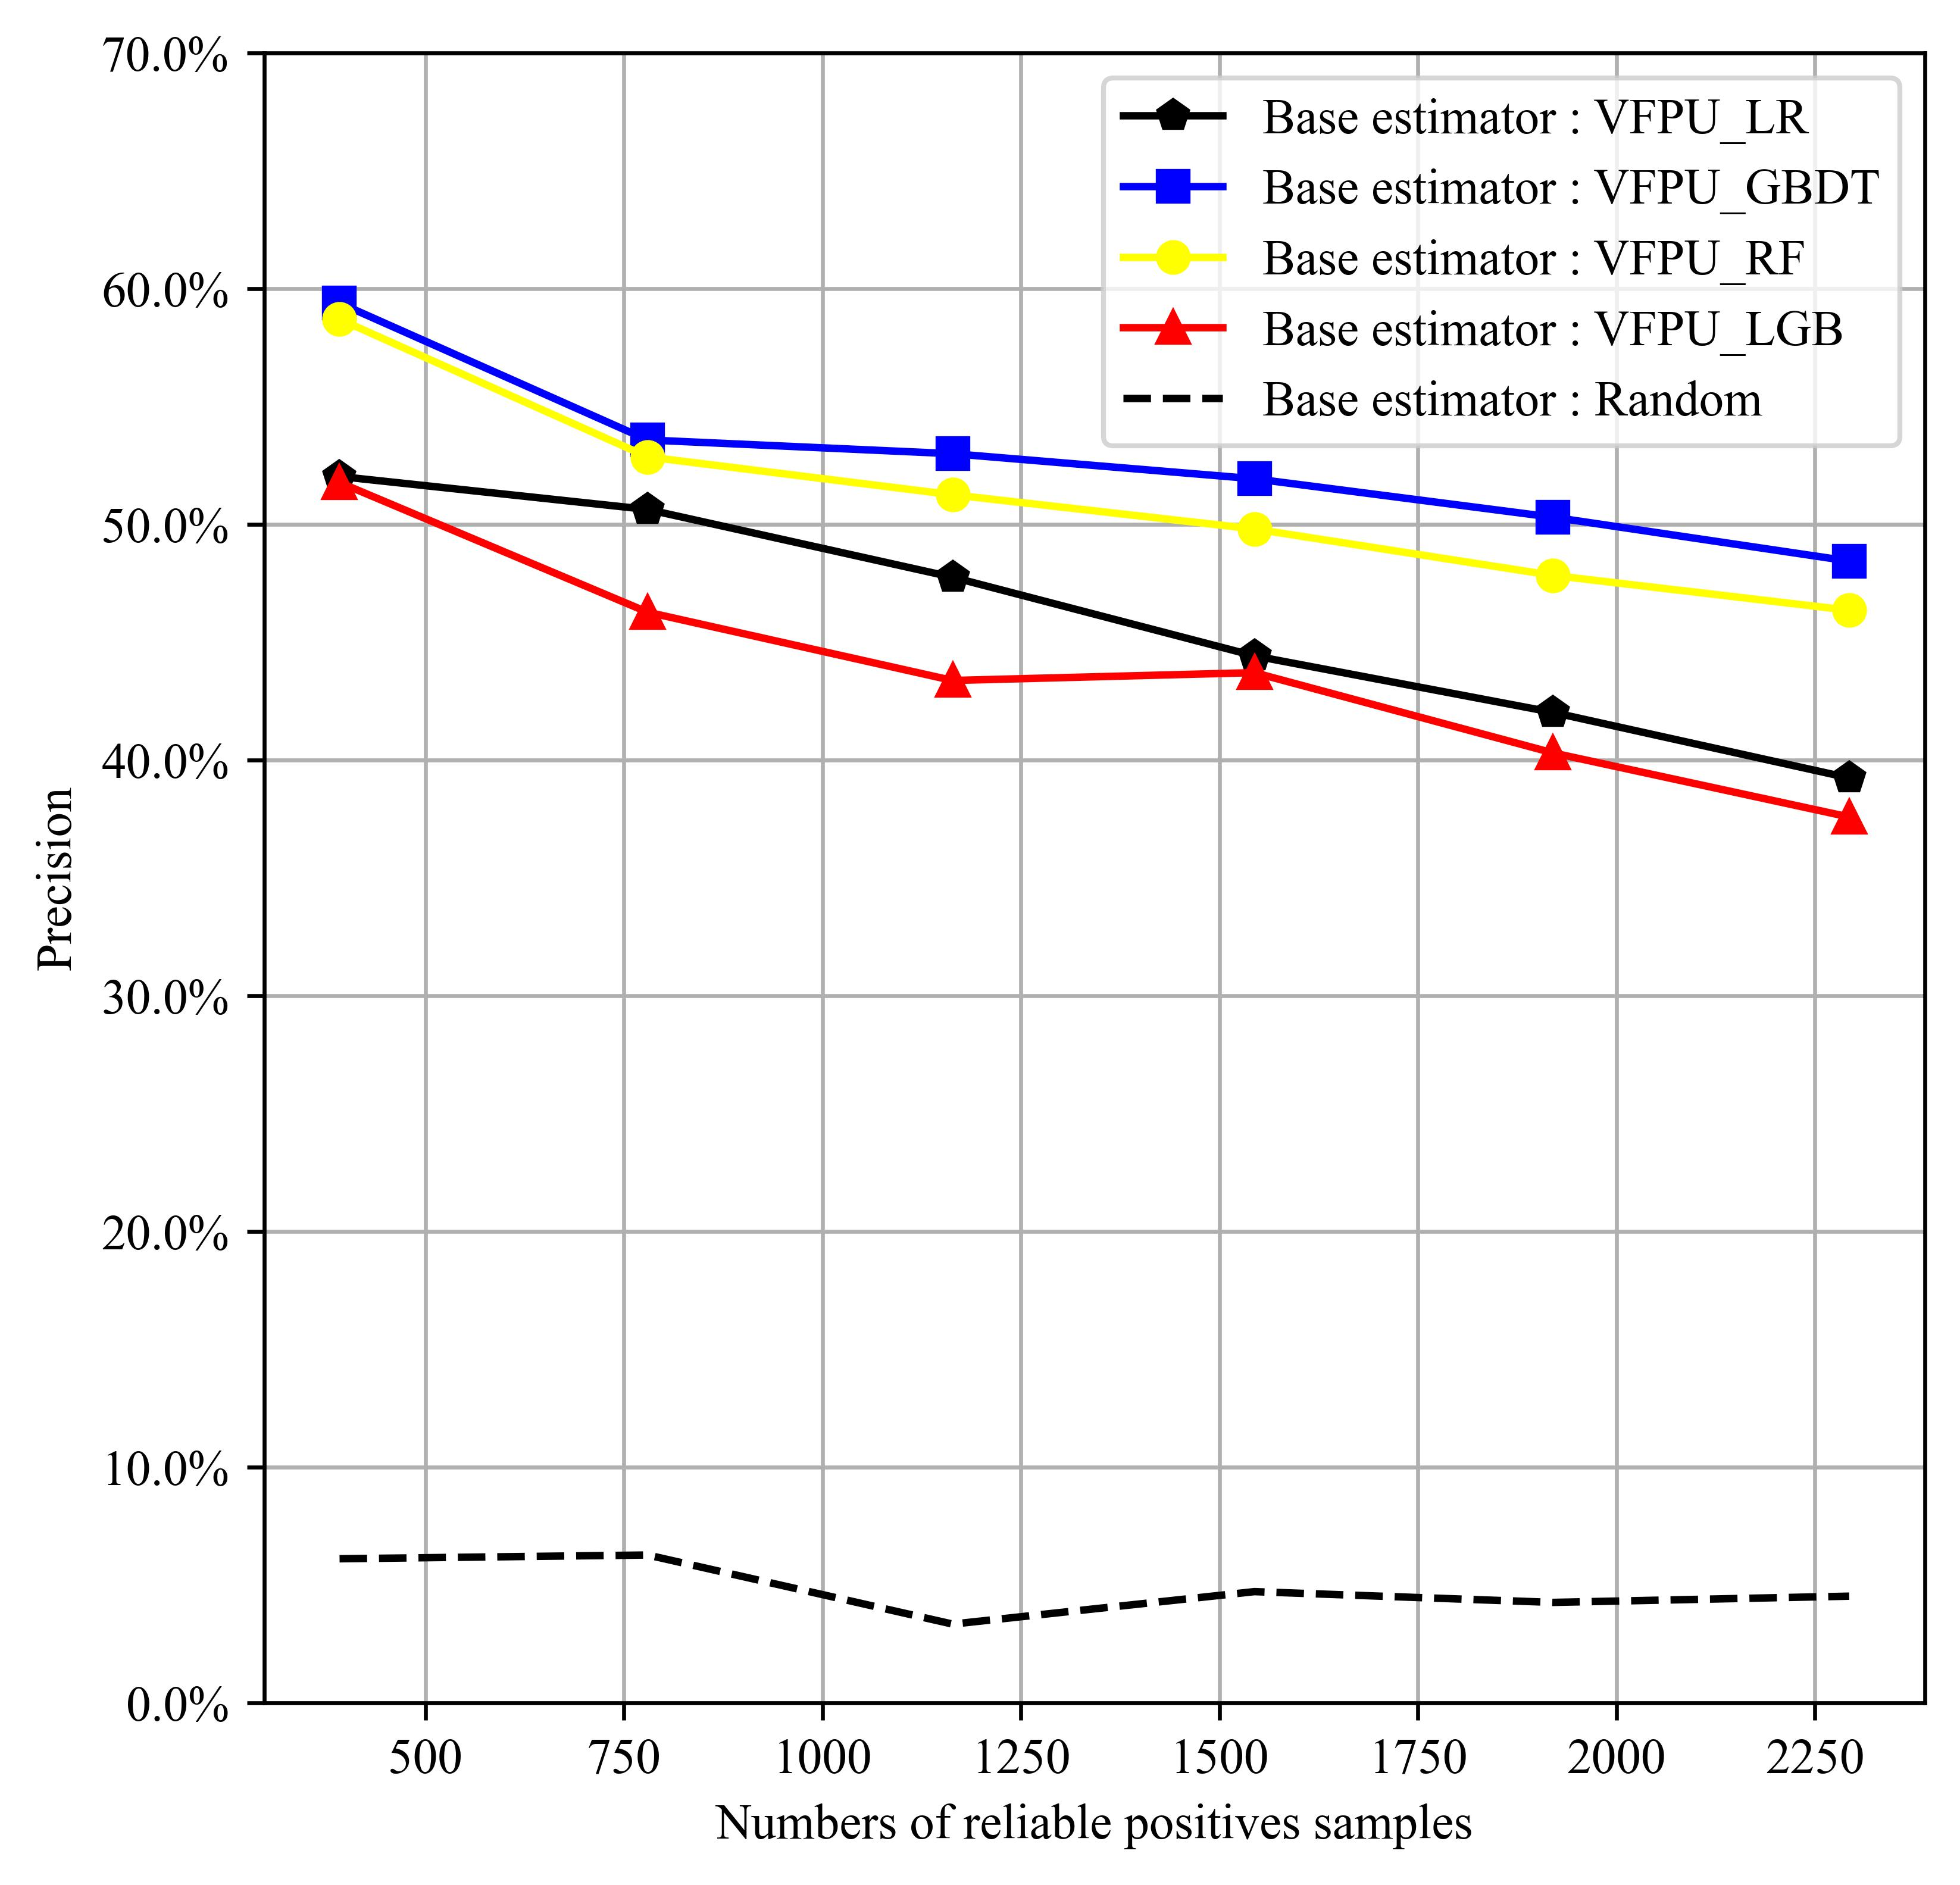
\includegraphics[width=0.45\textwidth,height=4.1cm]{chapters/imgs/Figure 2 (1) in JEPG format}}
	\subfigure[]{\label{RQ2.1.sub2}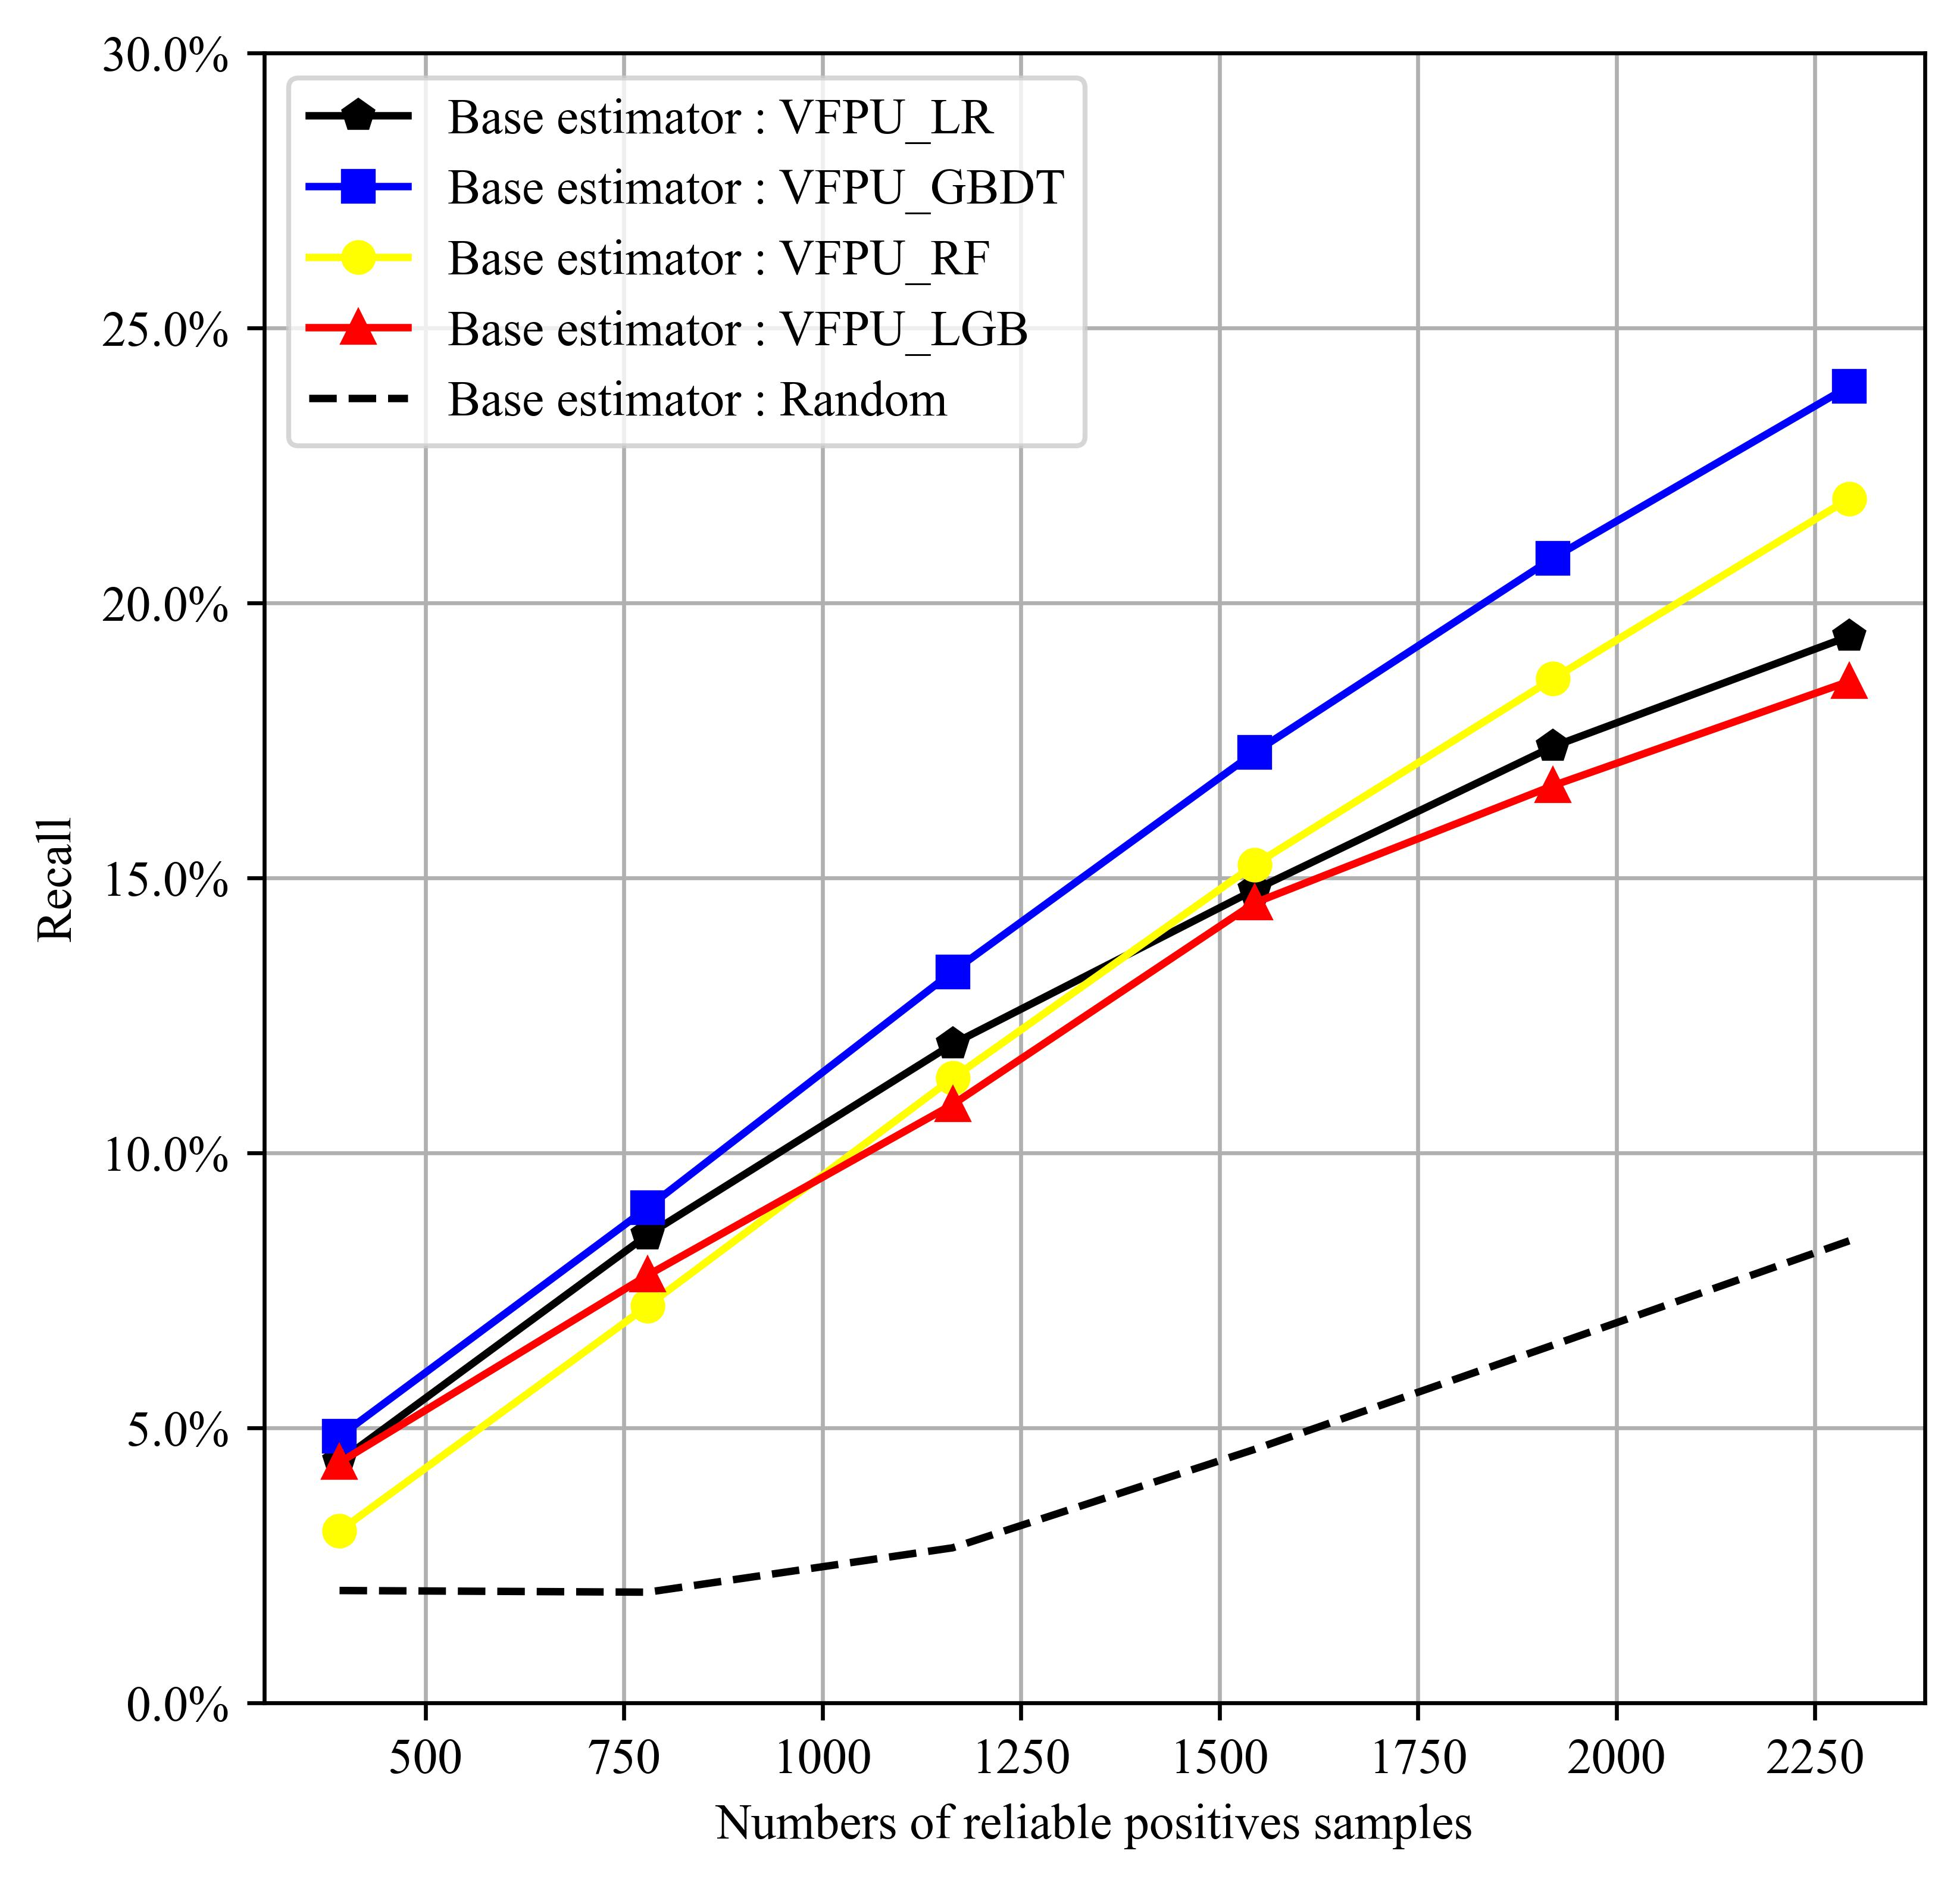
\includegraphics[width=0.45\textwidth,height=4.1cm]{chapters/imgs/Figure 2 (2) in JEPG format}}
	\subfigure[]{\label{RQ2.1.sub3}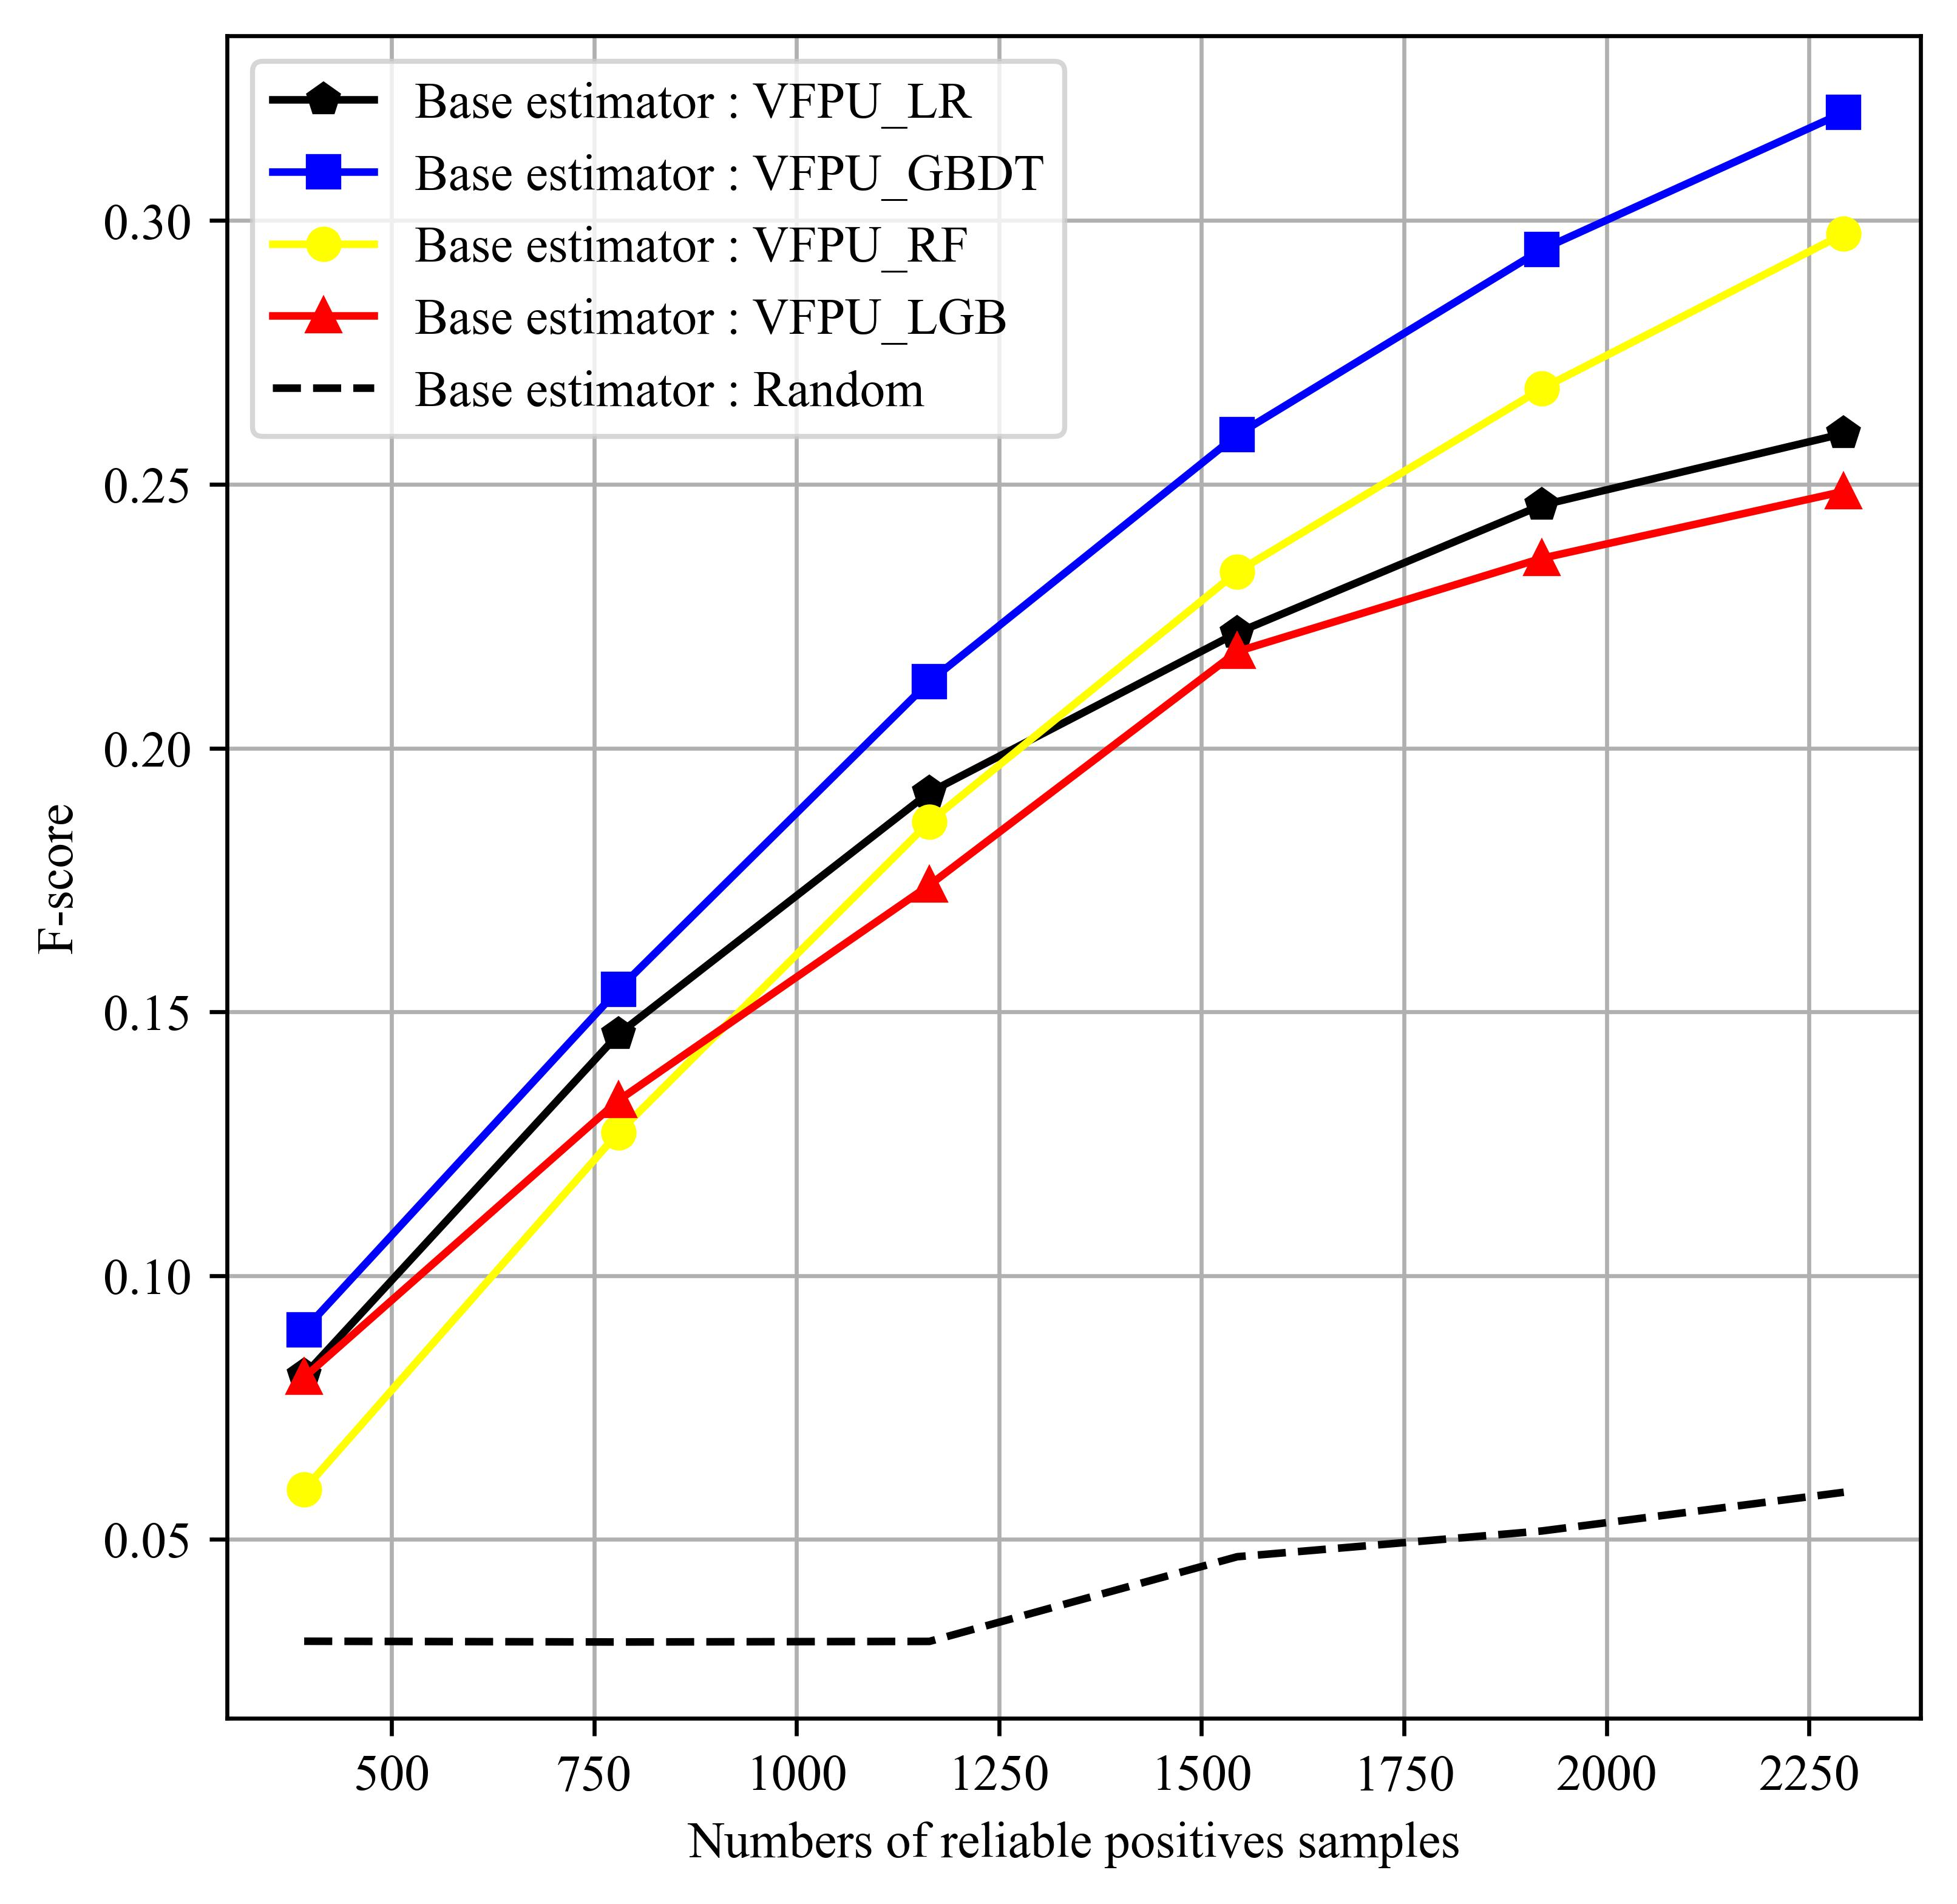
\includegraphics[width=0.45\textwidth,height=4.1cm]{chapters/imgs/Figure 2 (3) in JEPG format}}
	\subfigure[]{\label{RQ2.1.sub4}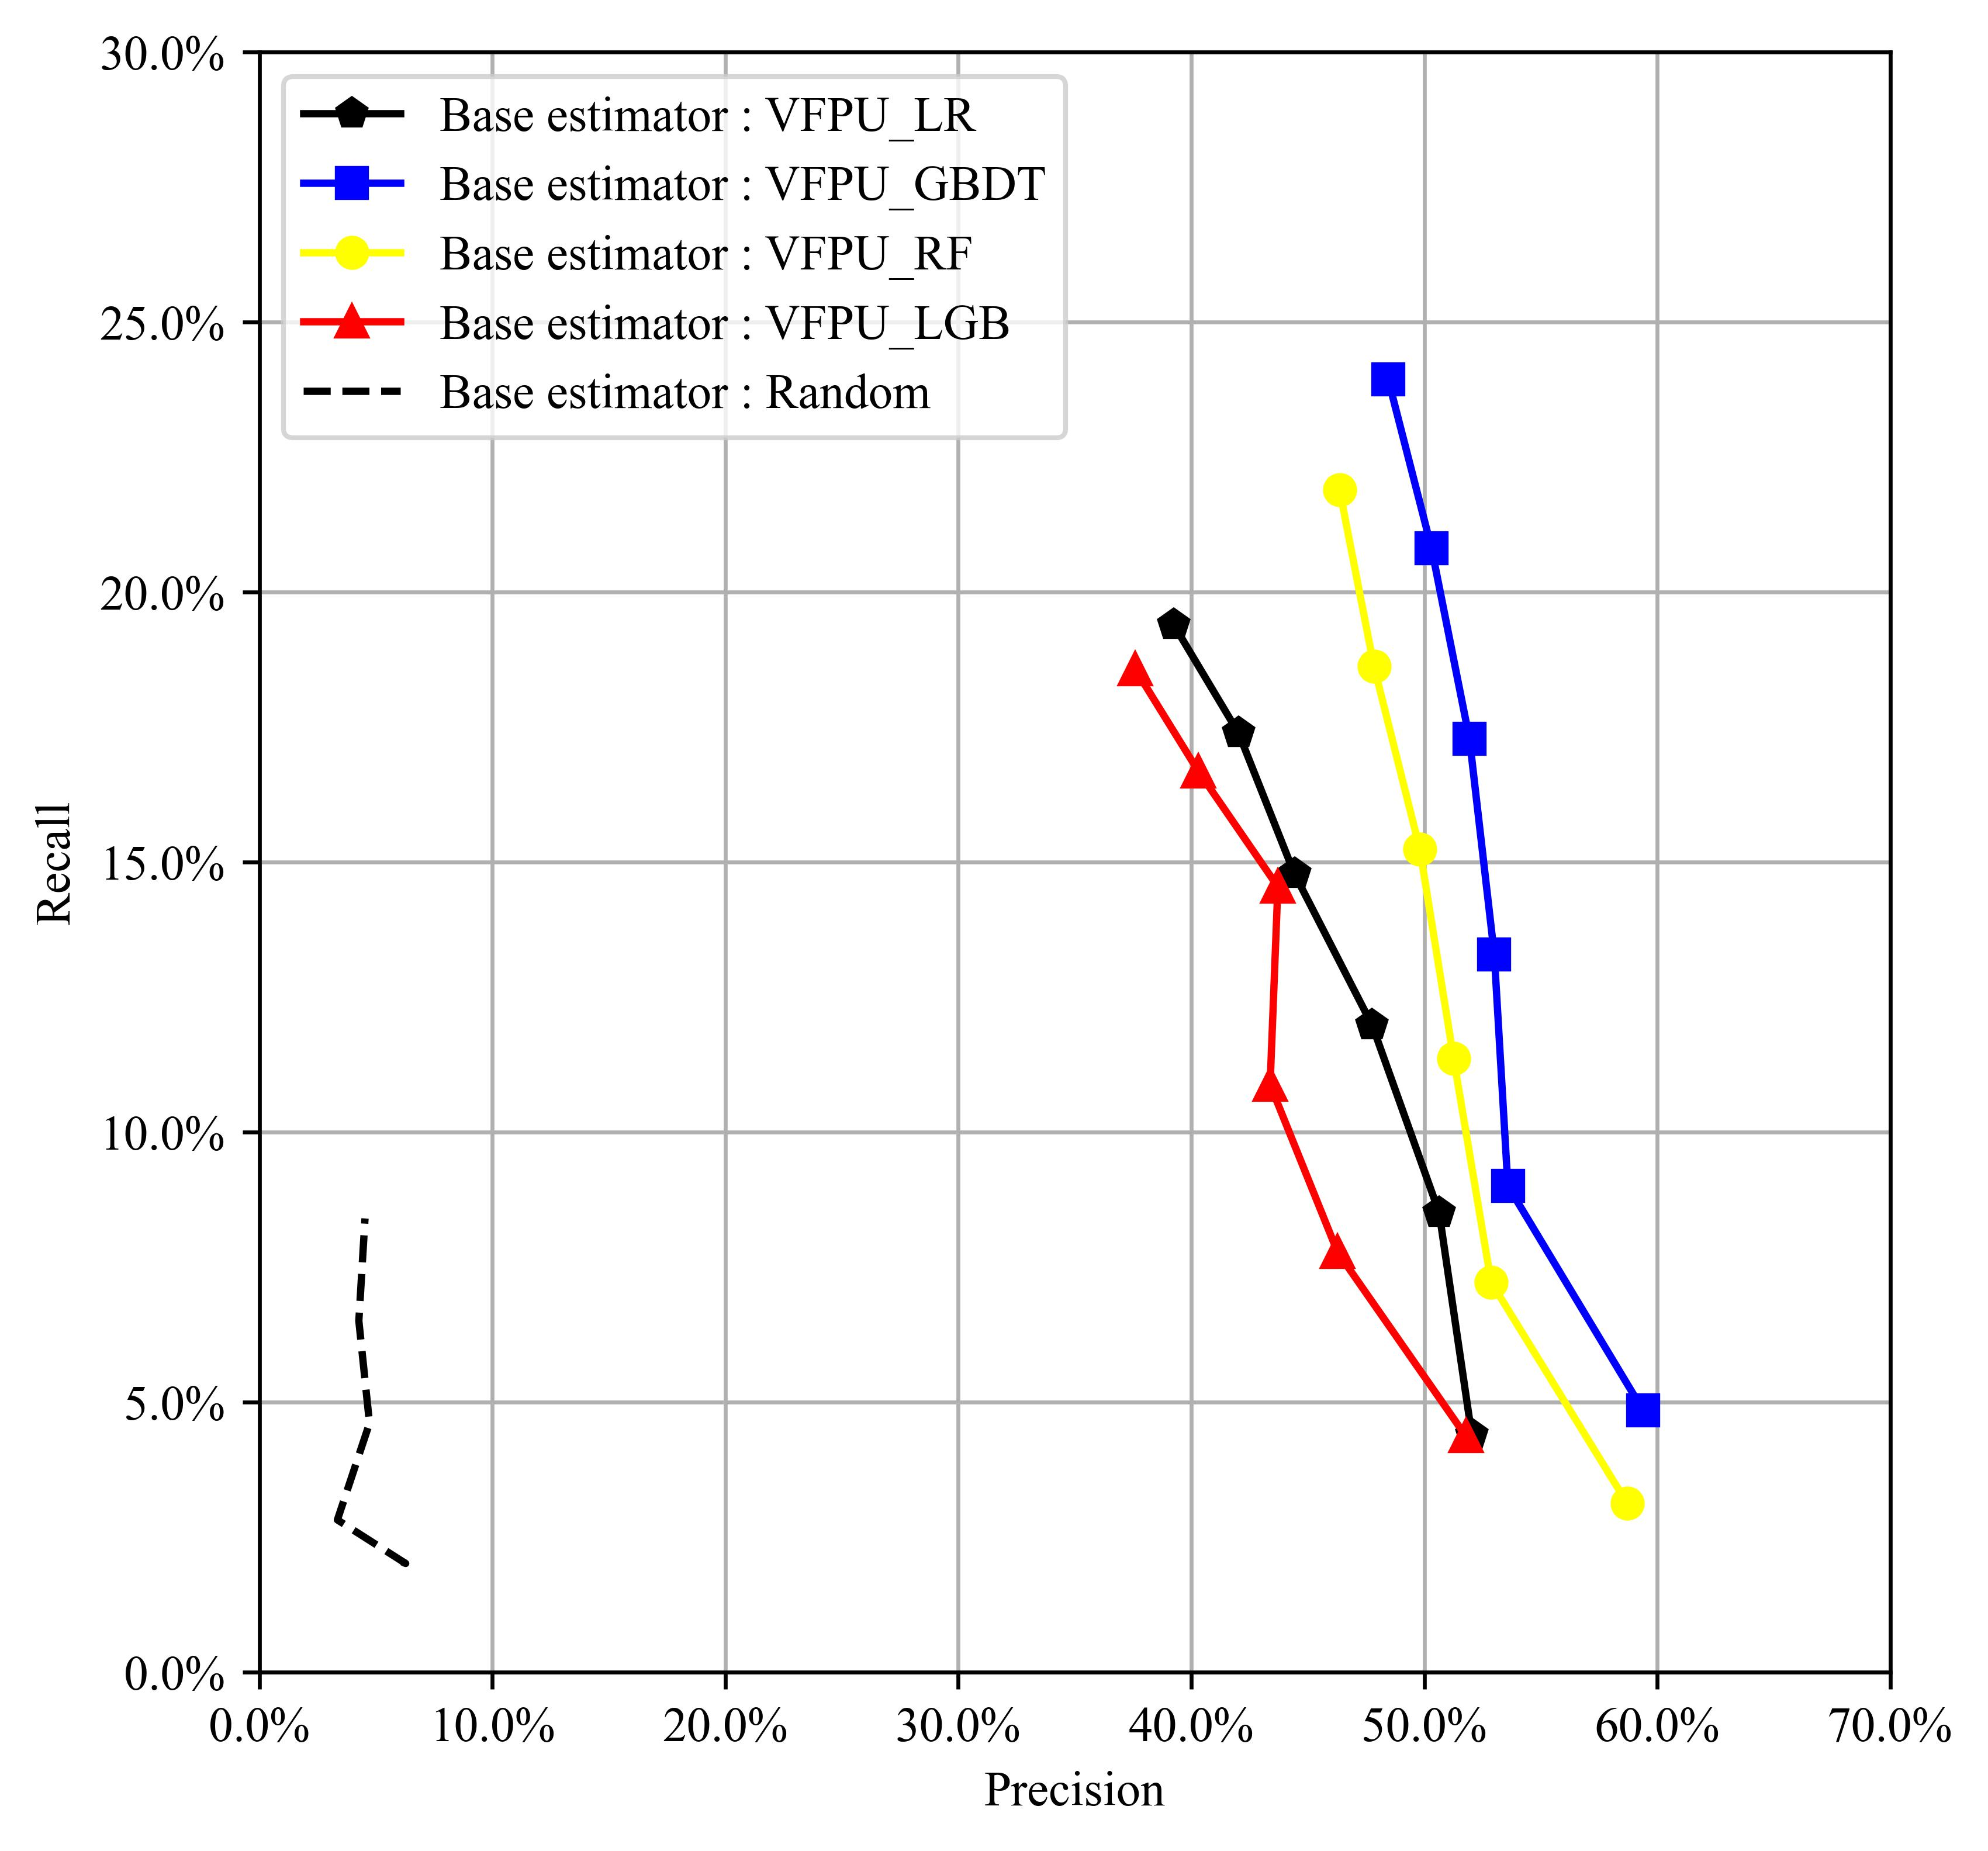
\includegraphics[width=0.45\textwidth,height=4.1cm]{chapters/imgs/Figure 2 (4) in JEPG format}}
	\bicaption[\xiaosi 不同基学器在不同可靠正样本数量下的性能]
	{\centering \songti \wuhao 不同基学器的性能:(a)精度;(b)召回率;(c)F-score;(d)精度-召回率(Bank)}
	{\centering \wuhao Base estimators performance: (a) Precision; (b) Recall; (c) F-score; (d) Precision-Recall}
	\label{RQ2.1}
\end{figure}

\vspace{-0.5cm} 


\begin{figure}[H]
	\centering
	\subfigure[]{\label{RQ2.2.sub1}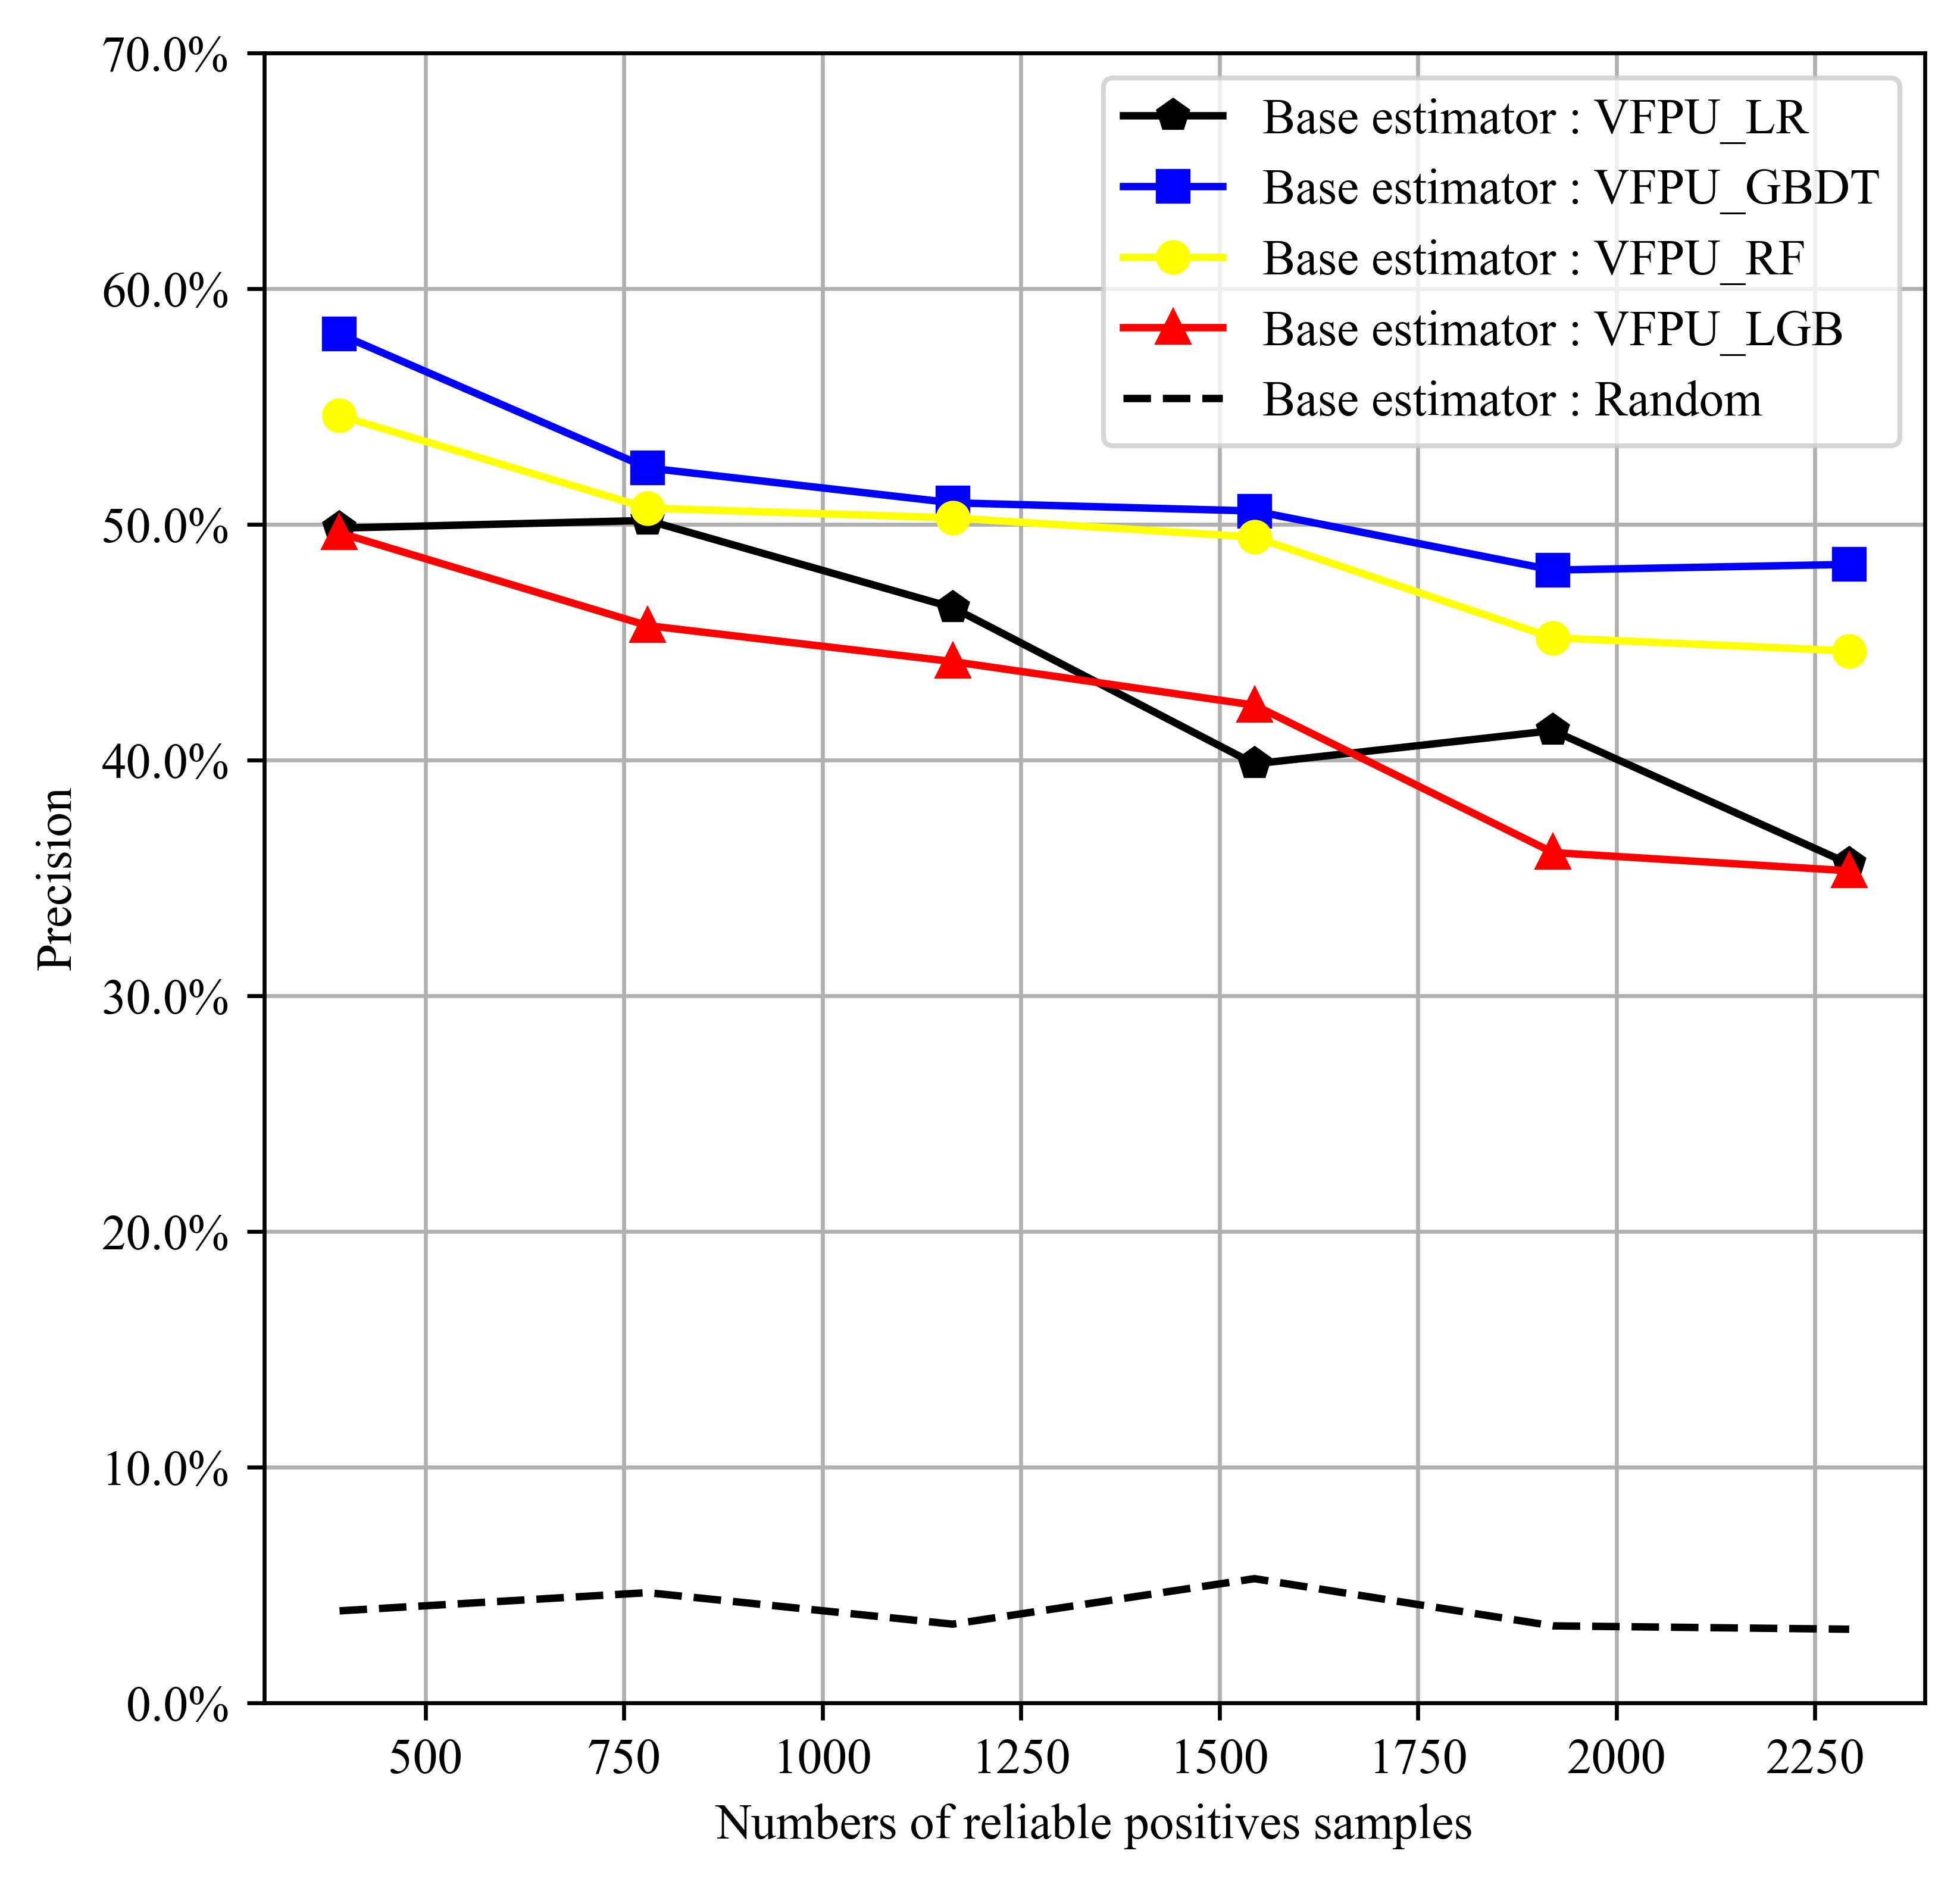
\includegraphics[width=0.45\textwidth,height=4.1cm]{chapters/imgs/Figure 3 (1) in JEPG format}}
	\subfigure[]{\label{RQ2.2.sub2}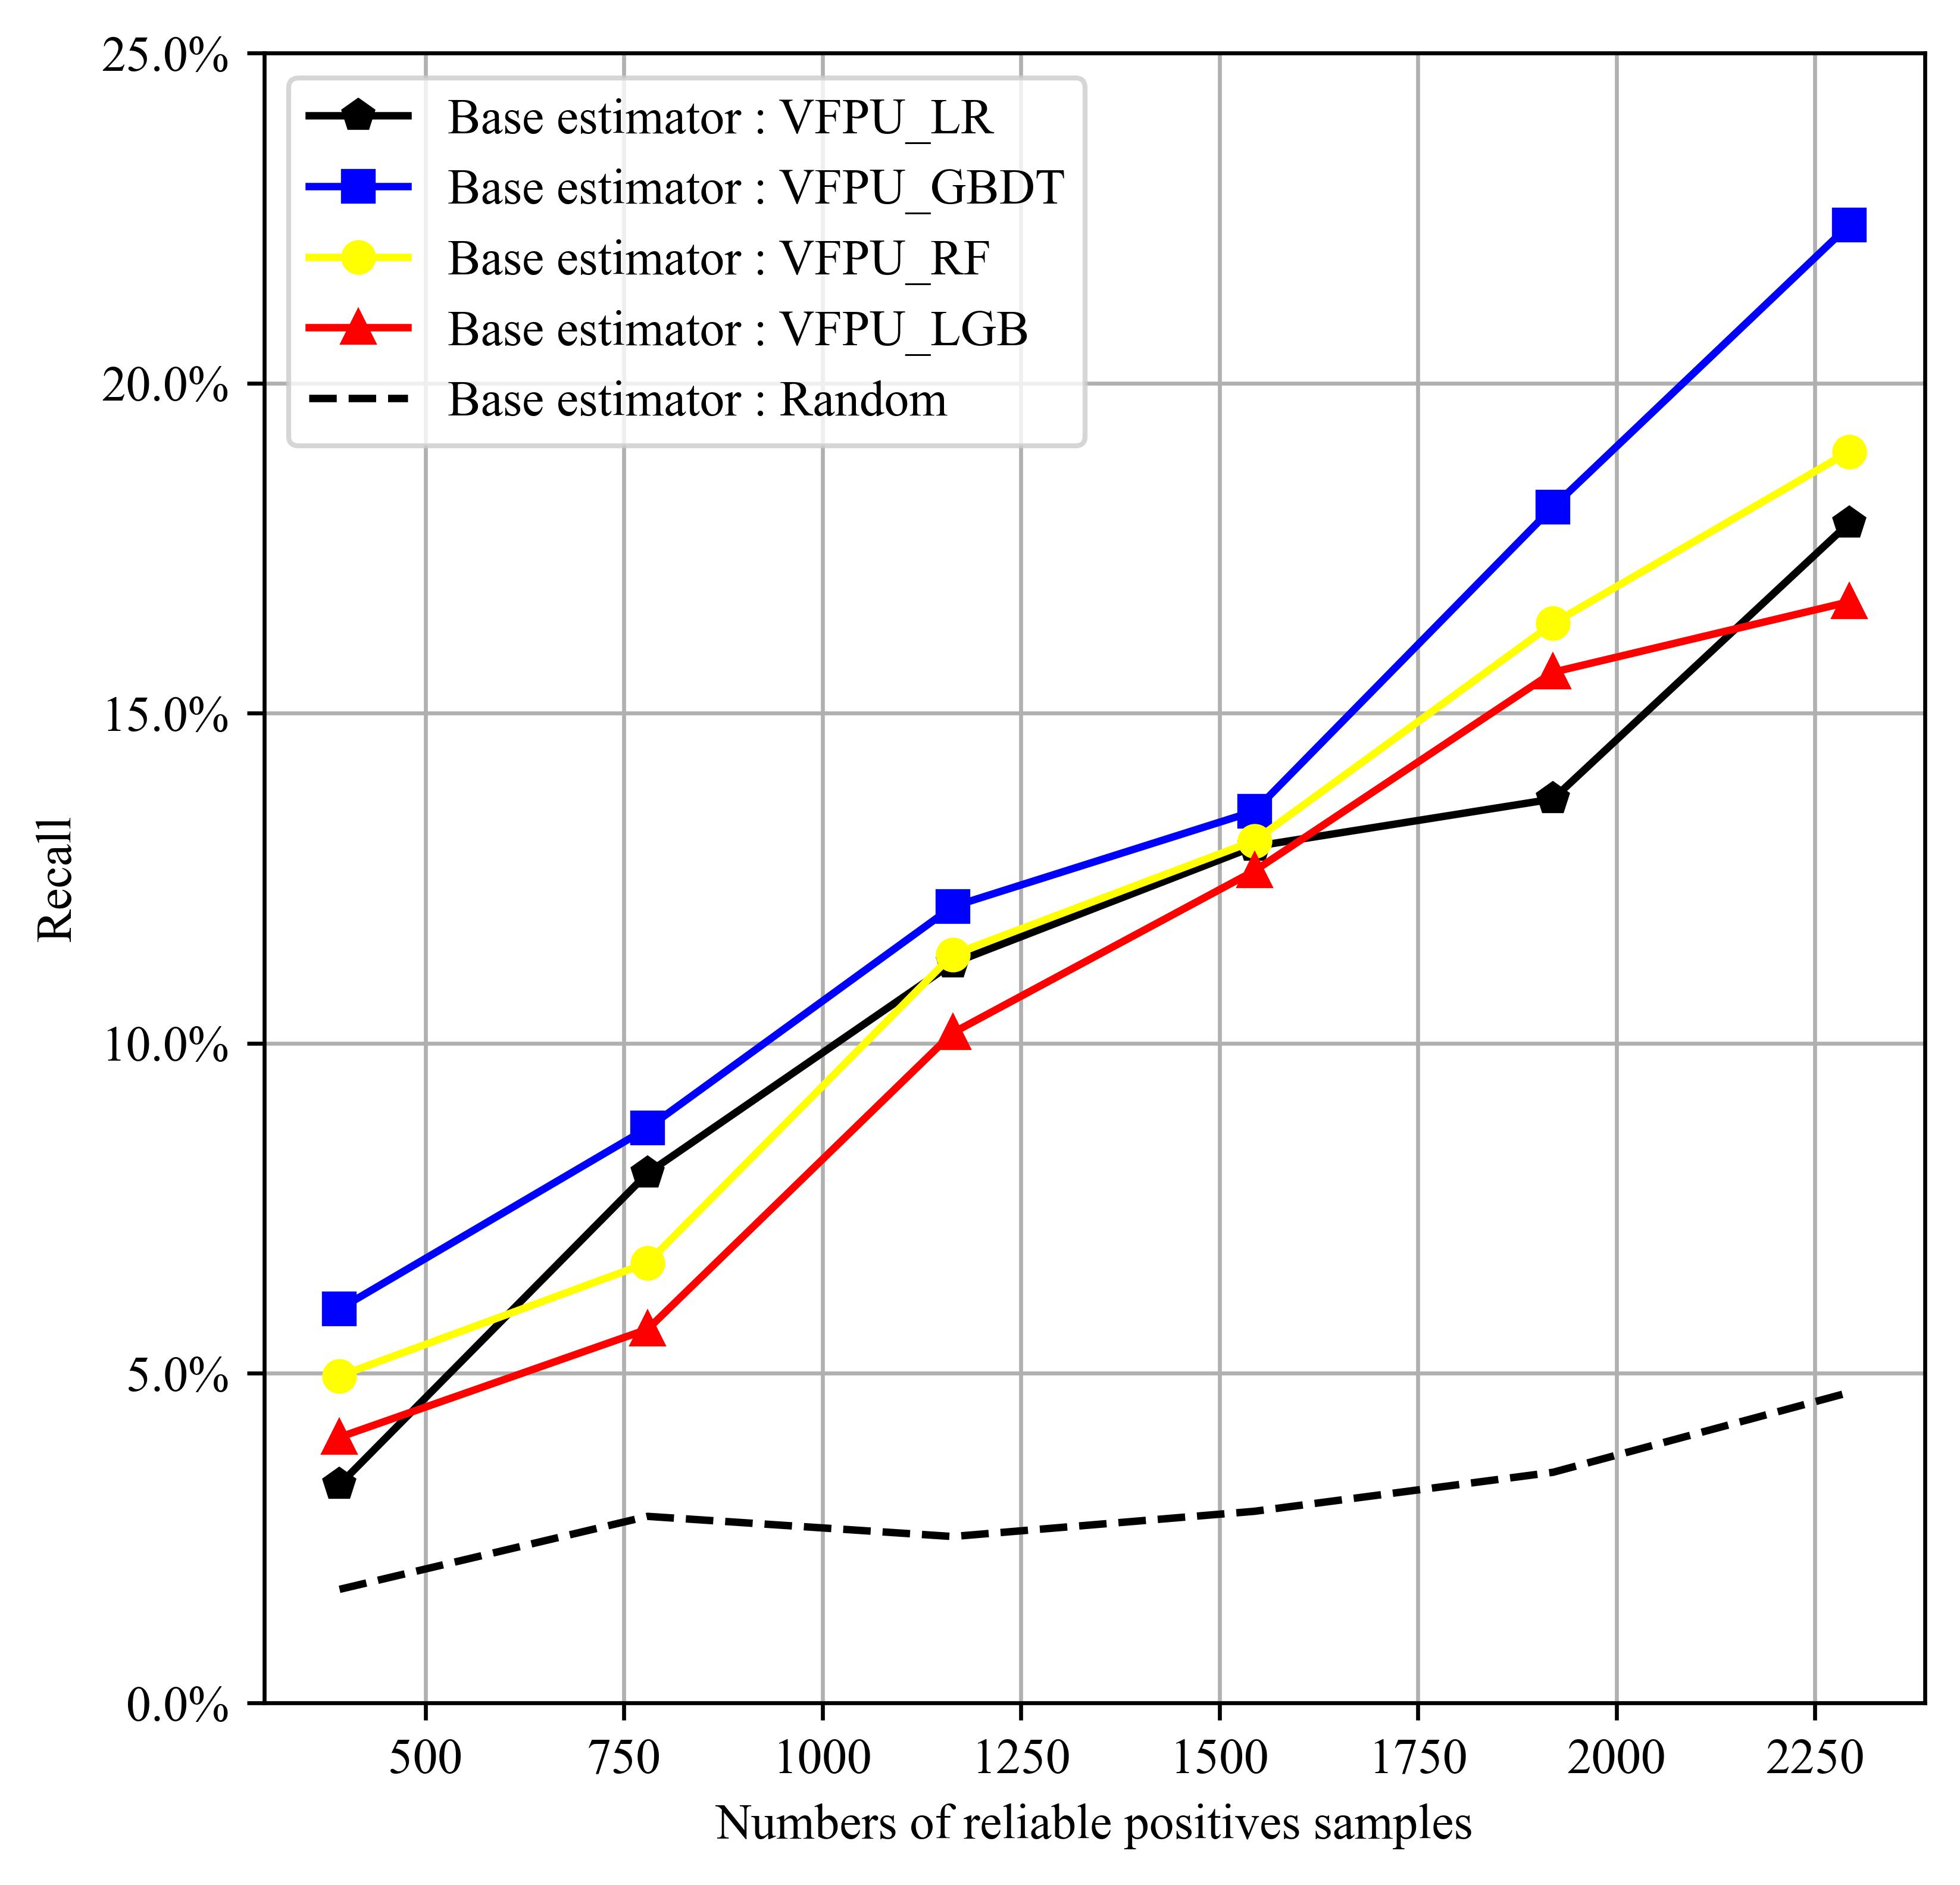
\includegraphics[width=0.45\textwidth,height=4.1cm]{chapters/imgs/Figure 3 (2) in JEPG format}}
	\subfigure[]{\label{RQ2.2.sub3}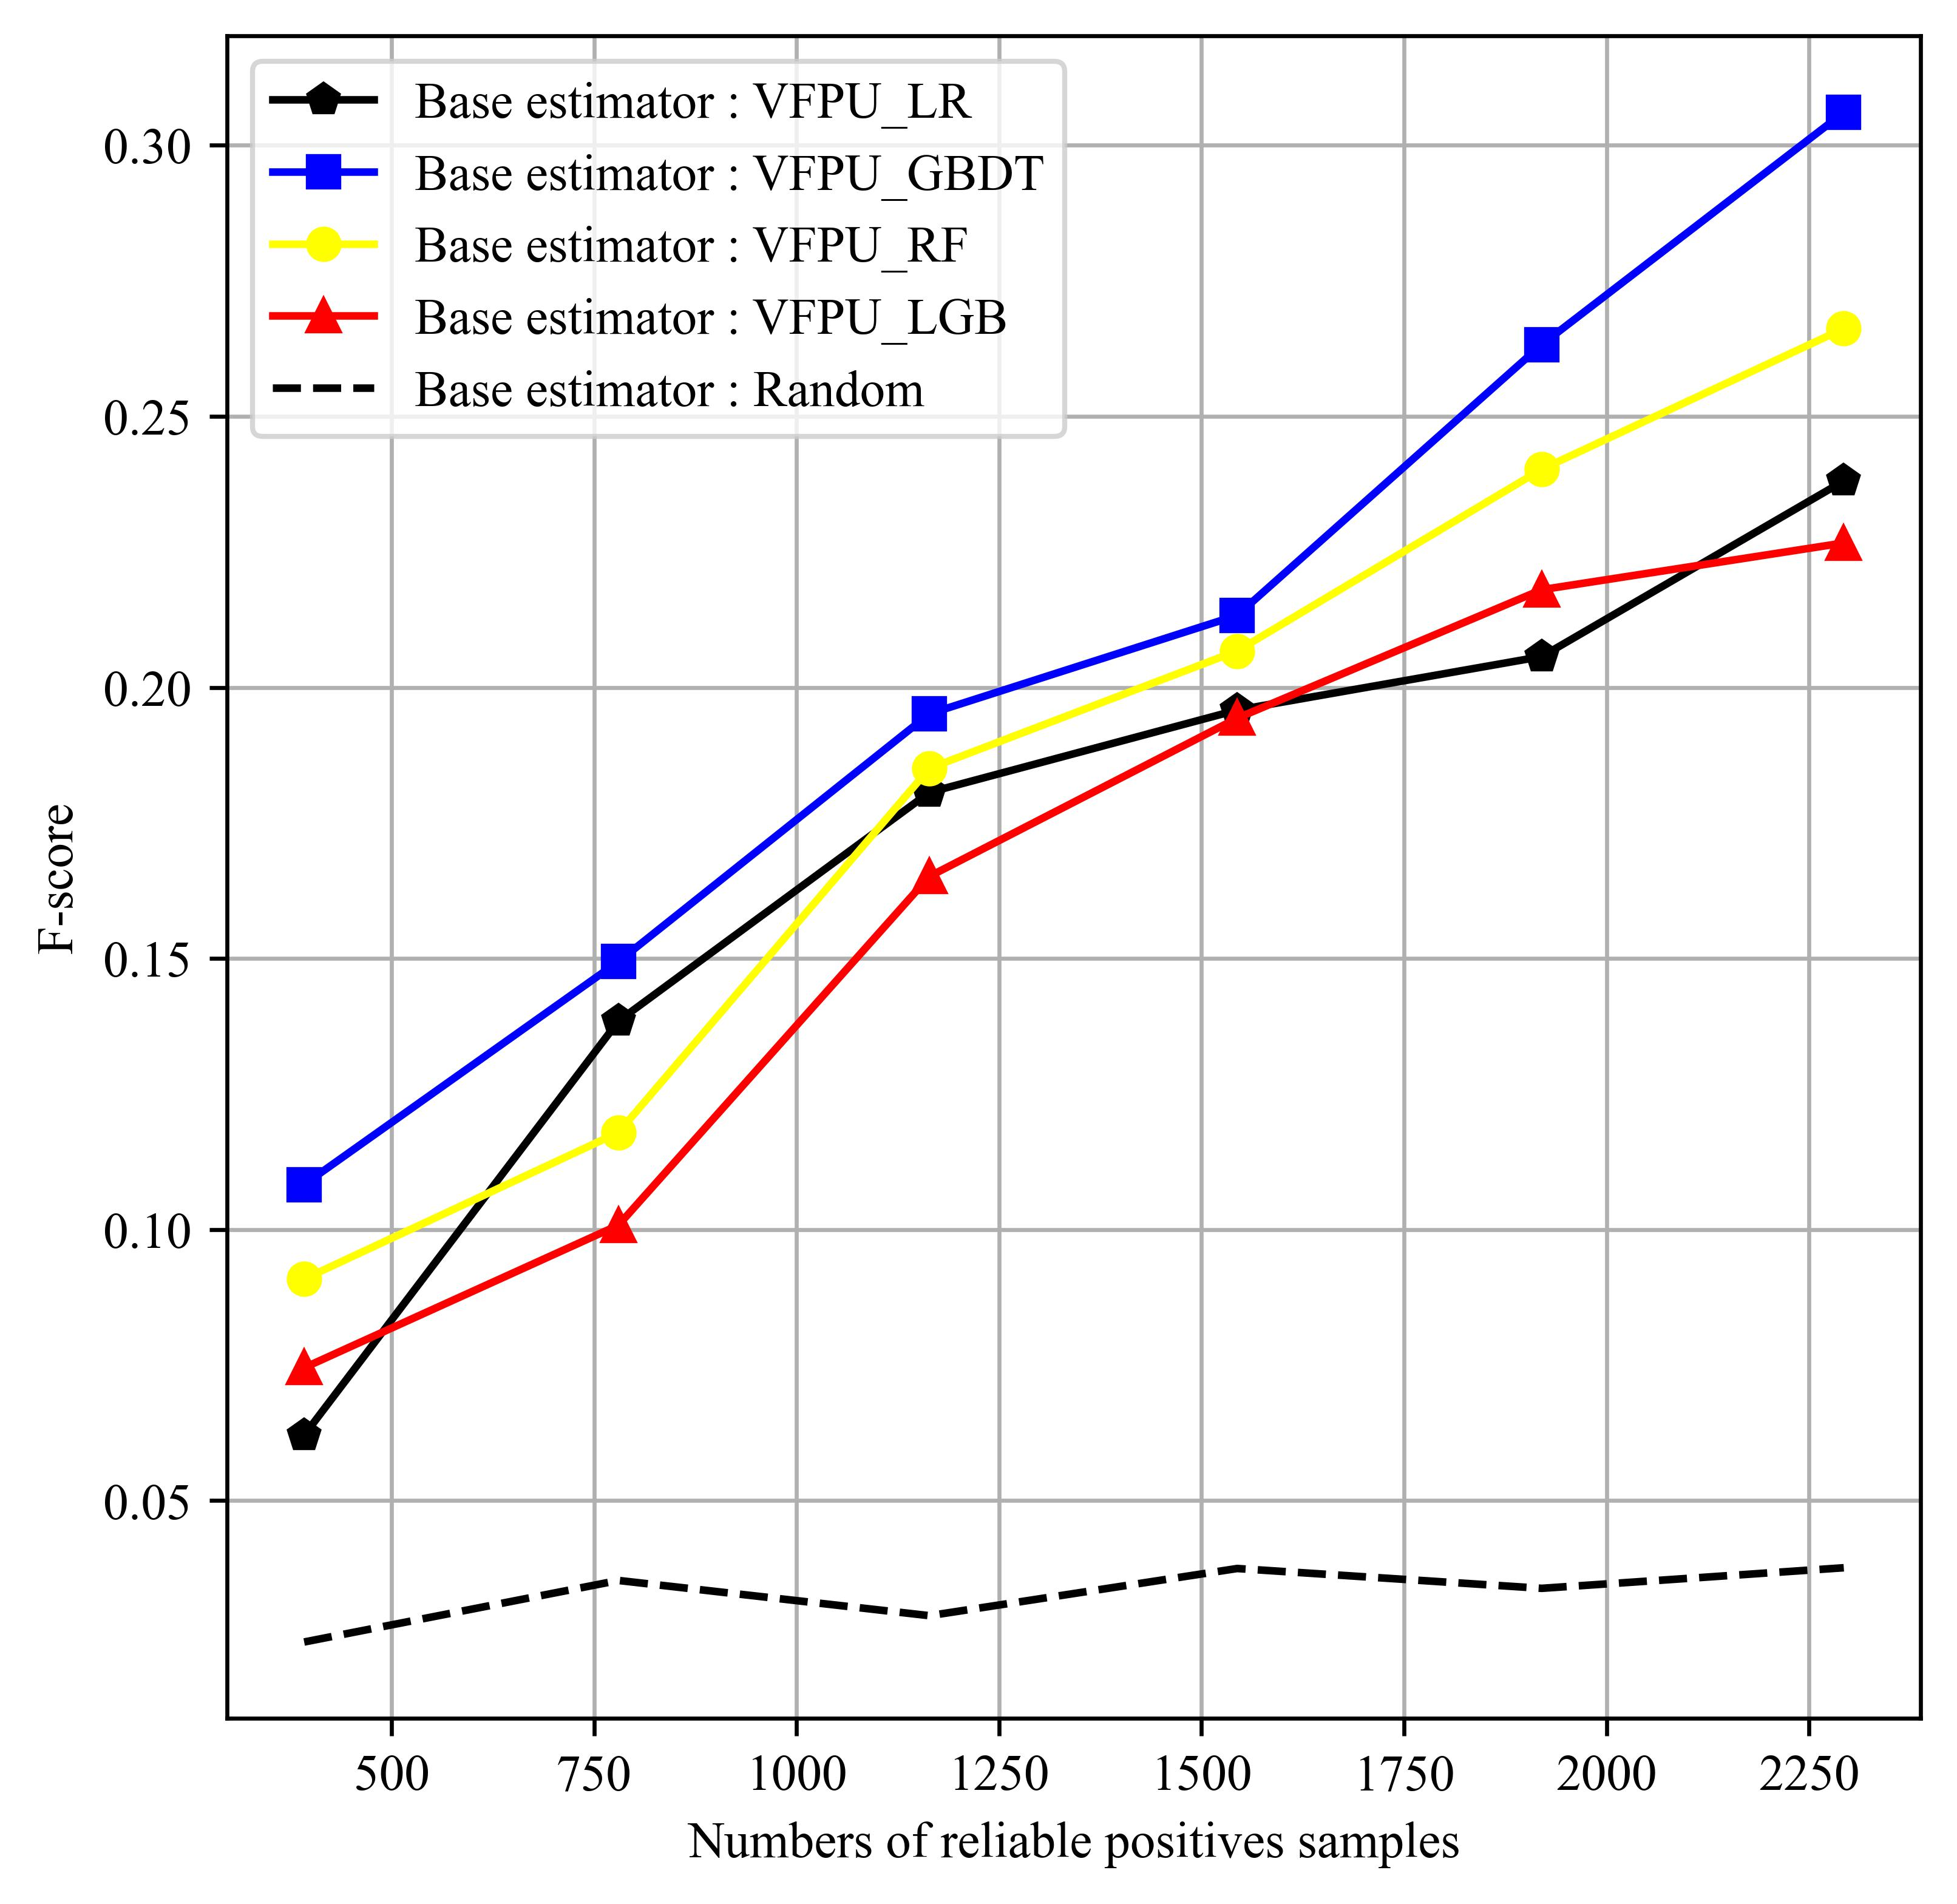
\includegraphics[width=0.45\textwidth,height=4.1cm]{chapters/imgs/Figure 3 (3) in JEPG format}}
	\subfigure[]{\label{RQ2.2.sub4}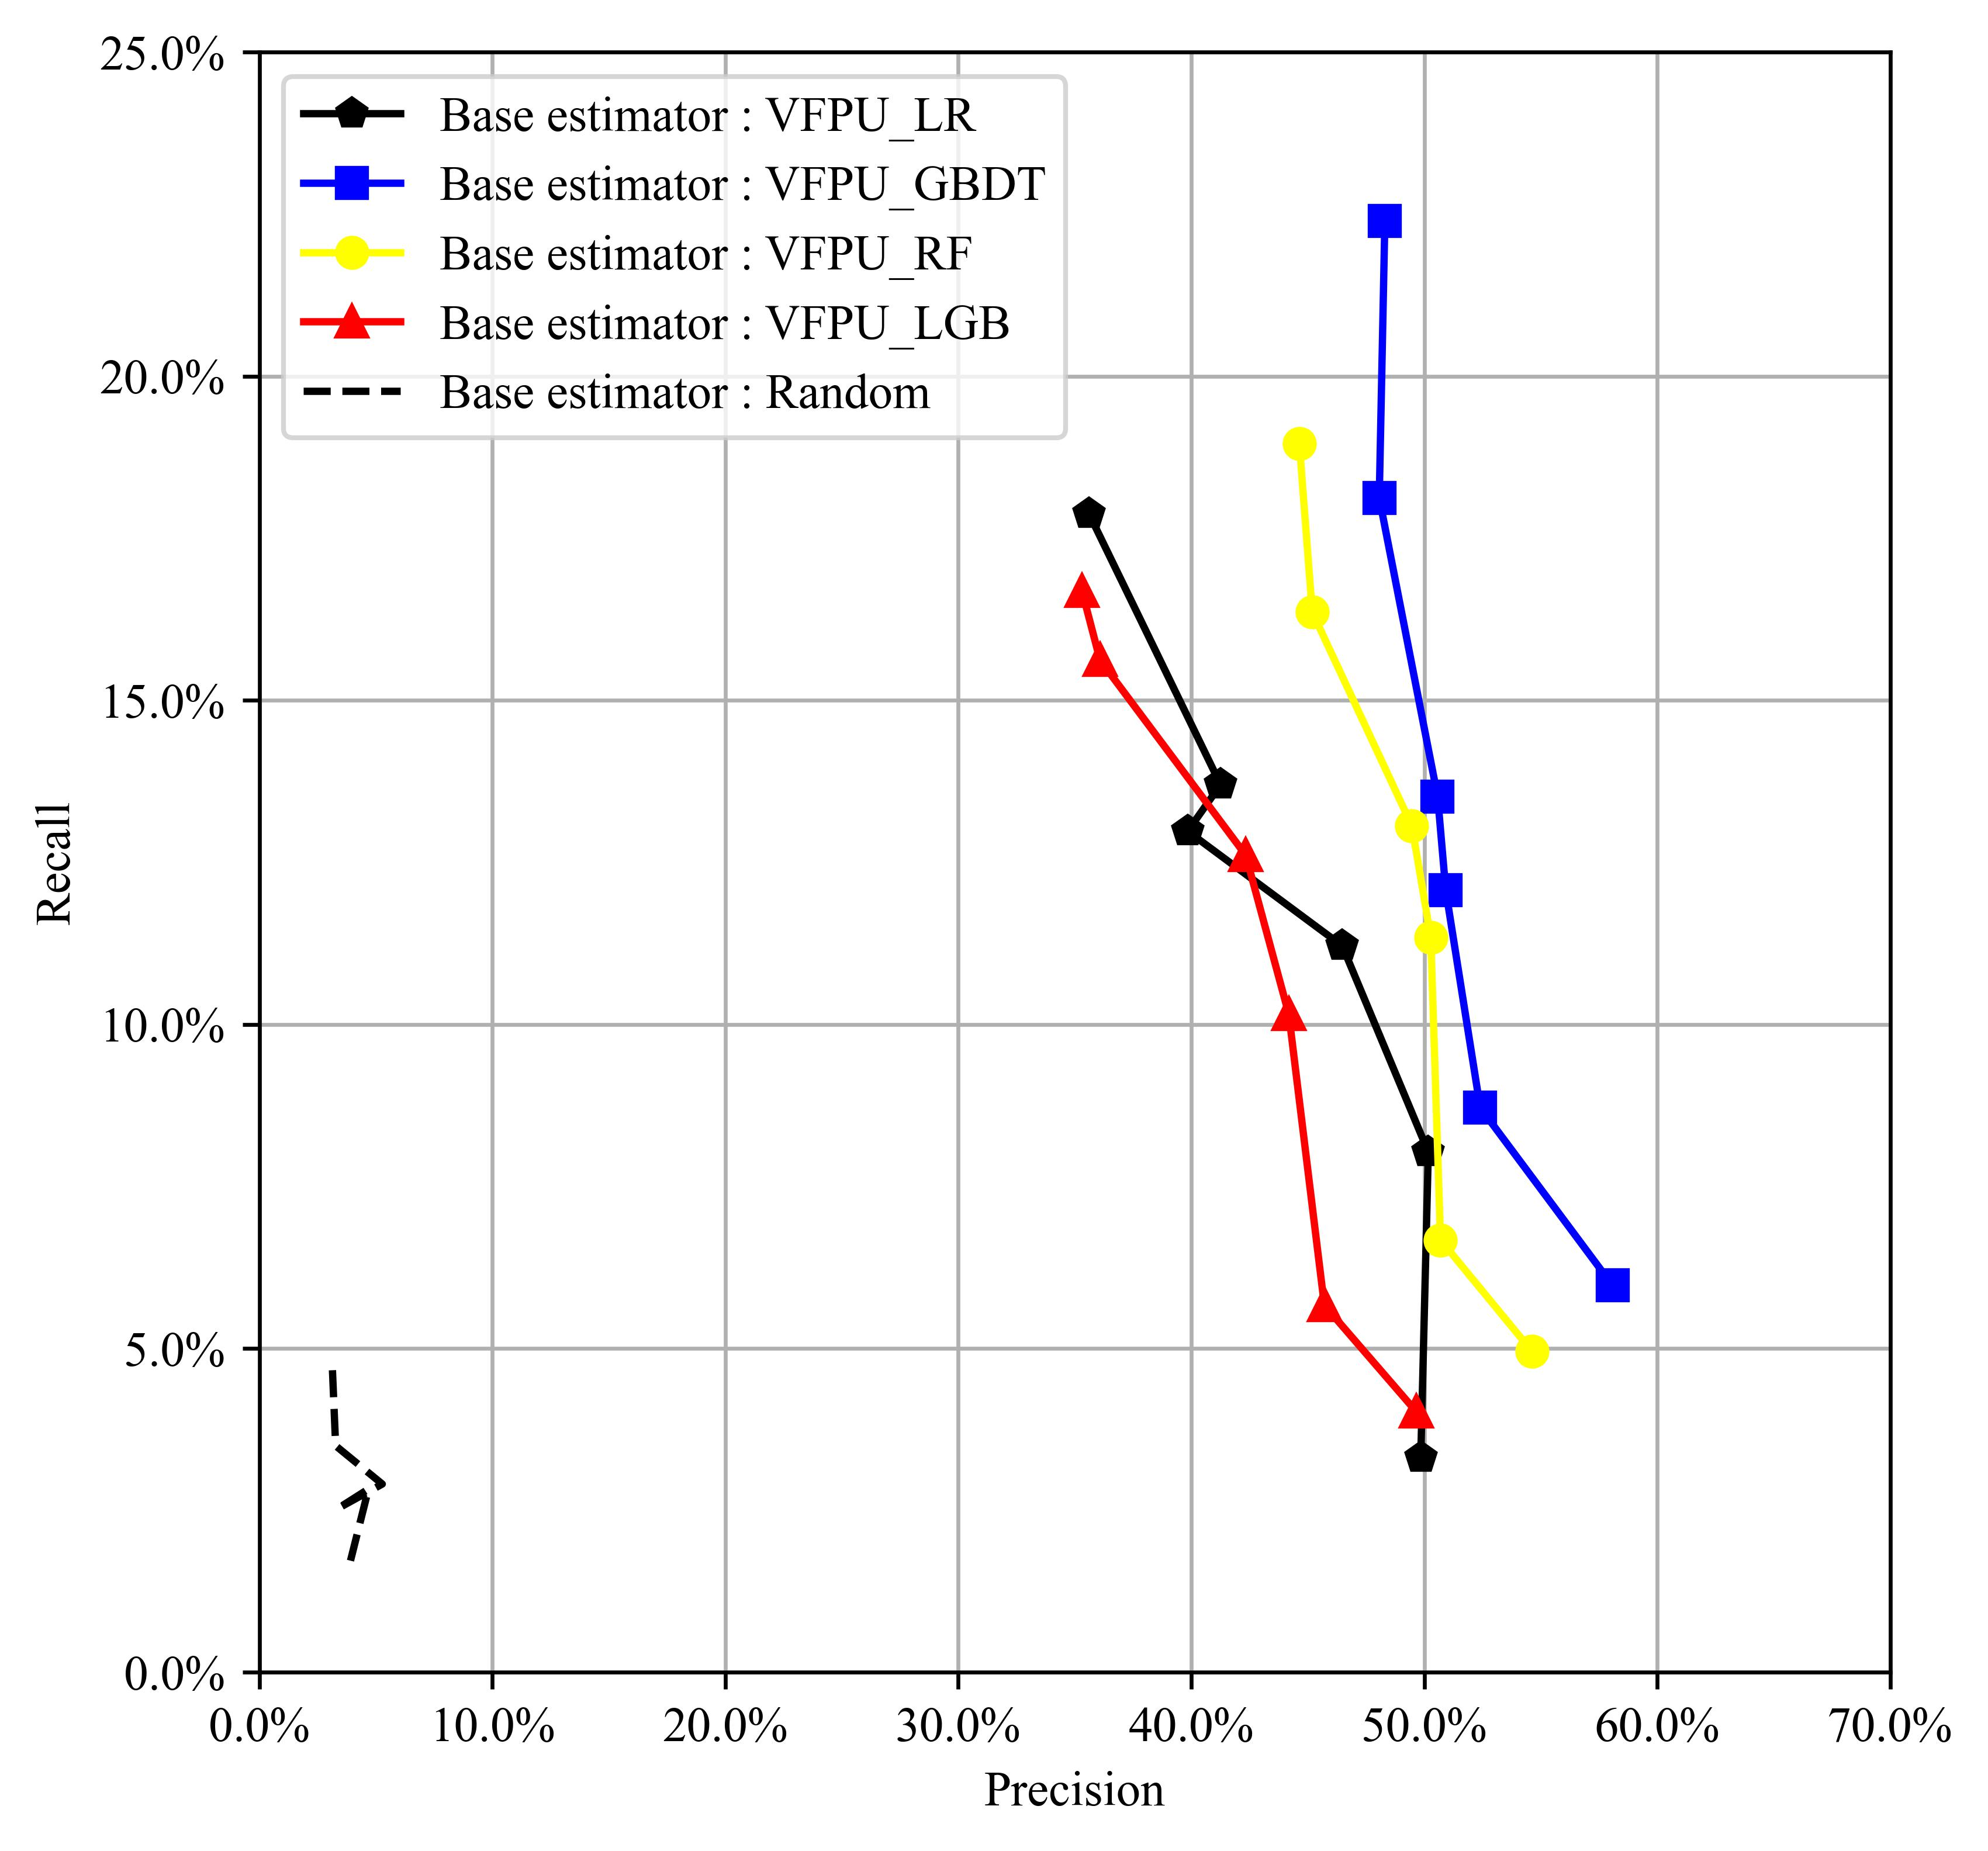
\includegraphics[width=0.45\textwidth,height=4.1cm]{chapters/imgs/Figure 3 (4) in JEPG format}}
	
	\bicaption[\xiaosi 不同基学器在不同可靠正样本数量下的性能]
	{\centering \songti \wuhao 不同基学器的性能:(a)精度;(b)召回率;(c)F-score;(d)精度-召回率(Credit)}
	{\centering \wuhao Base estimators performance: (a) Precision; (b) Recall; (c) F-score; (d) Precision-Recall}
	\label{RQ2.2}
\end{figure}

\vspace{-0.1cm}
\begin{figure}[h]
	\centering
	\subfigure[]{\label{RQ2.3.sub1}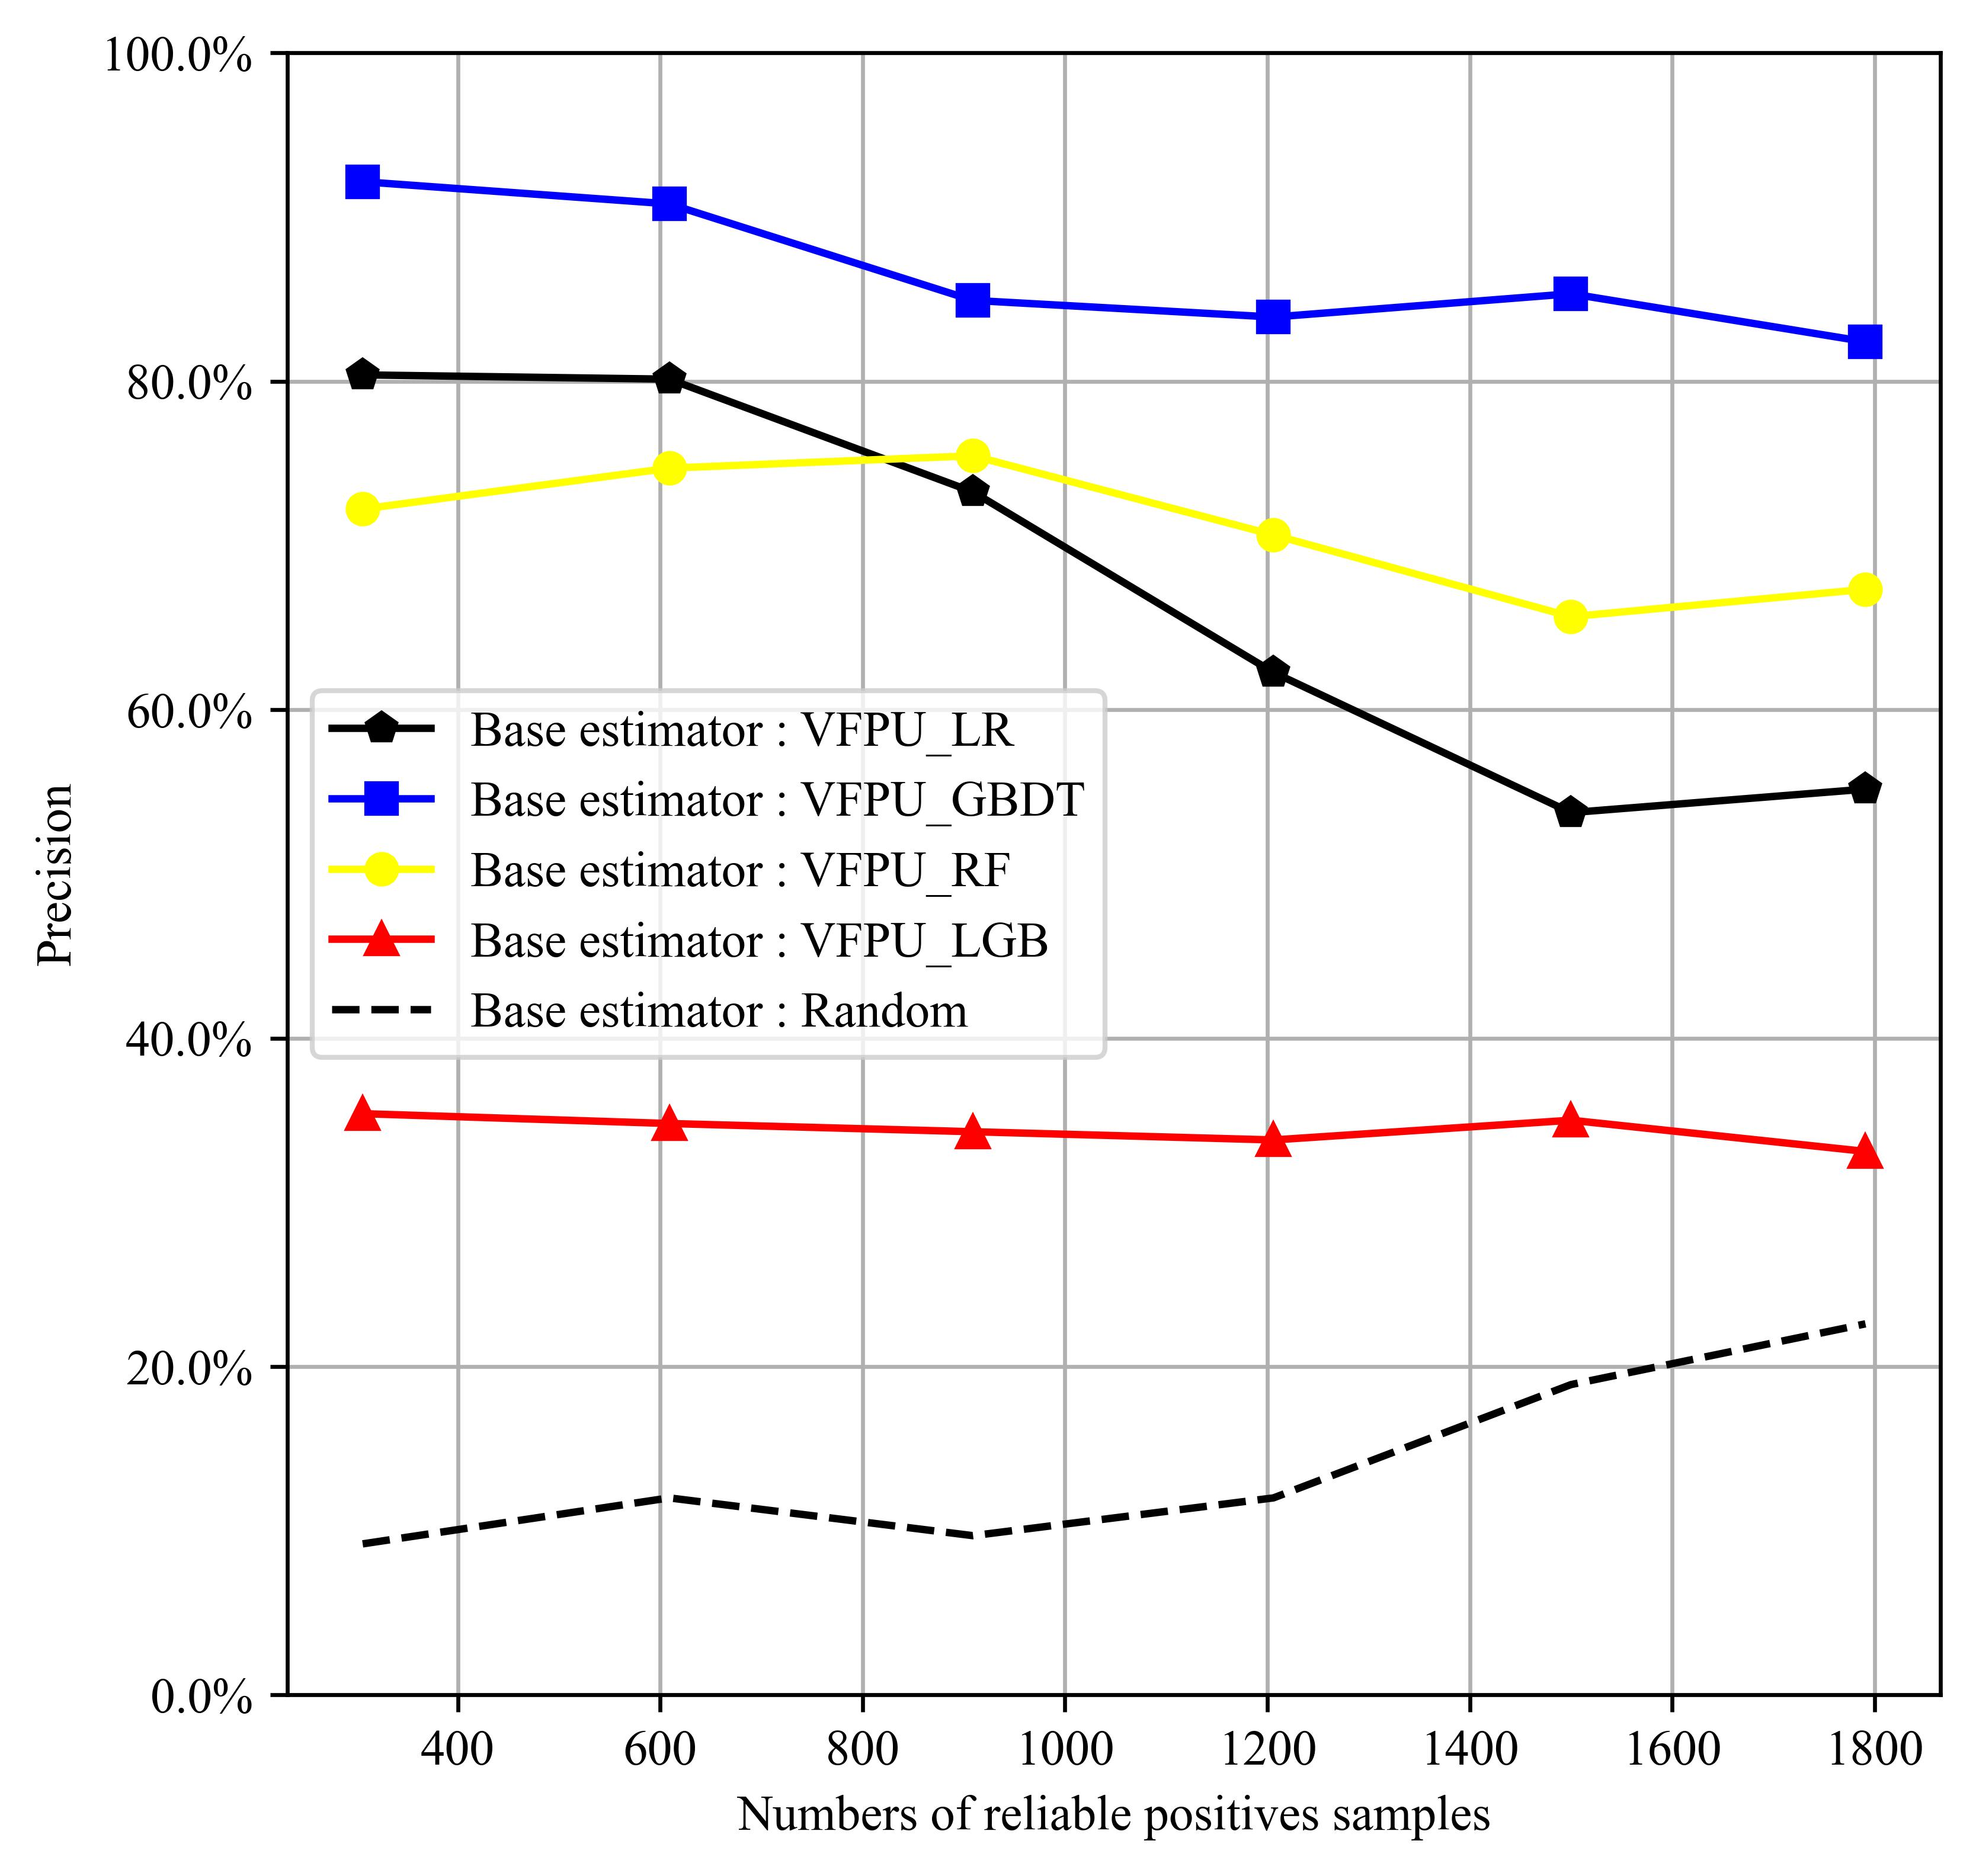
\includegraphics[width=0.45\textwidth,height=4.1cm]{chapters/imgs/Figure 4 (1) in JEPG format}}
	\subfigure[]{\label{RQ2.3.sub2}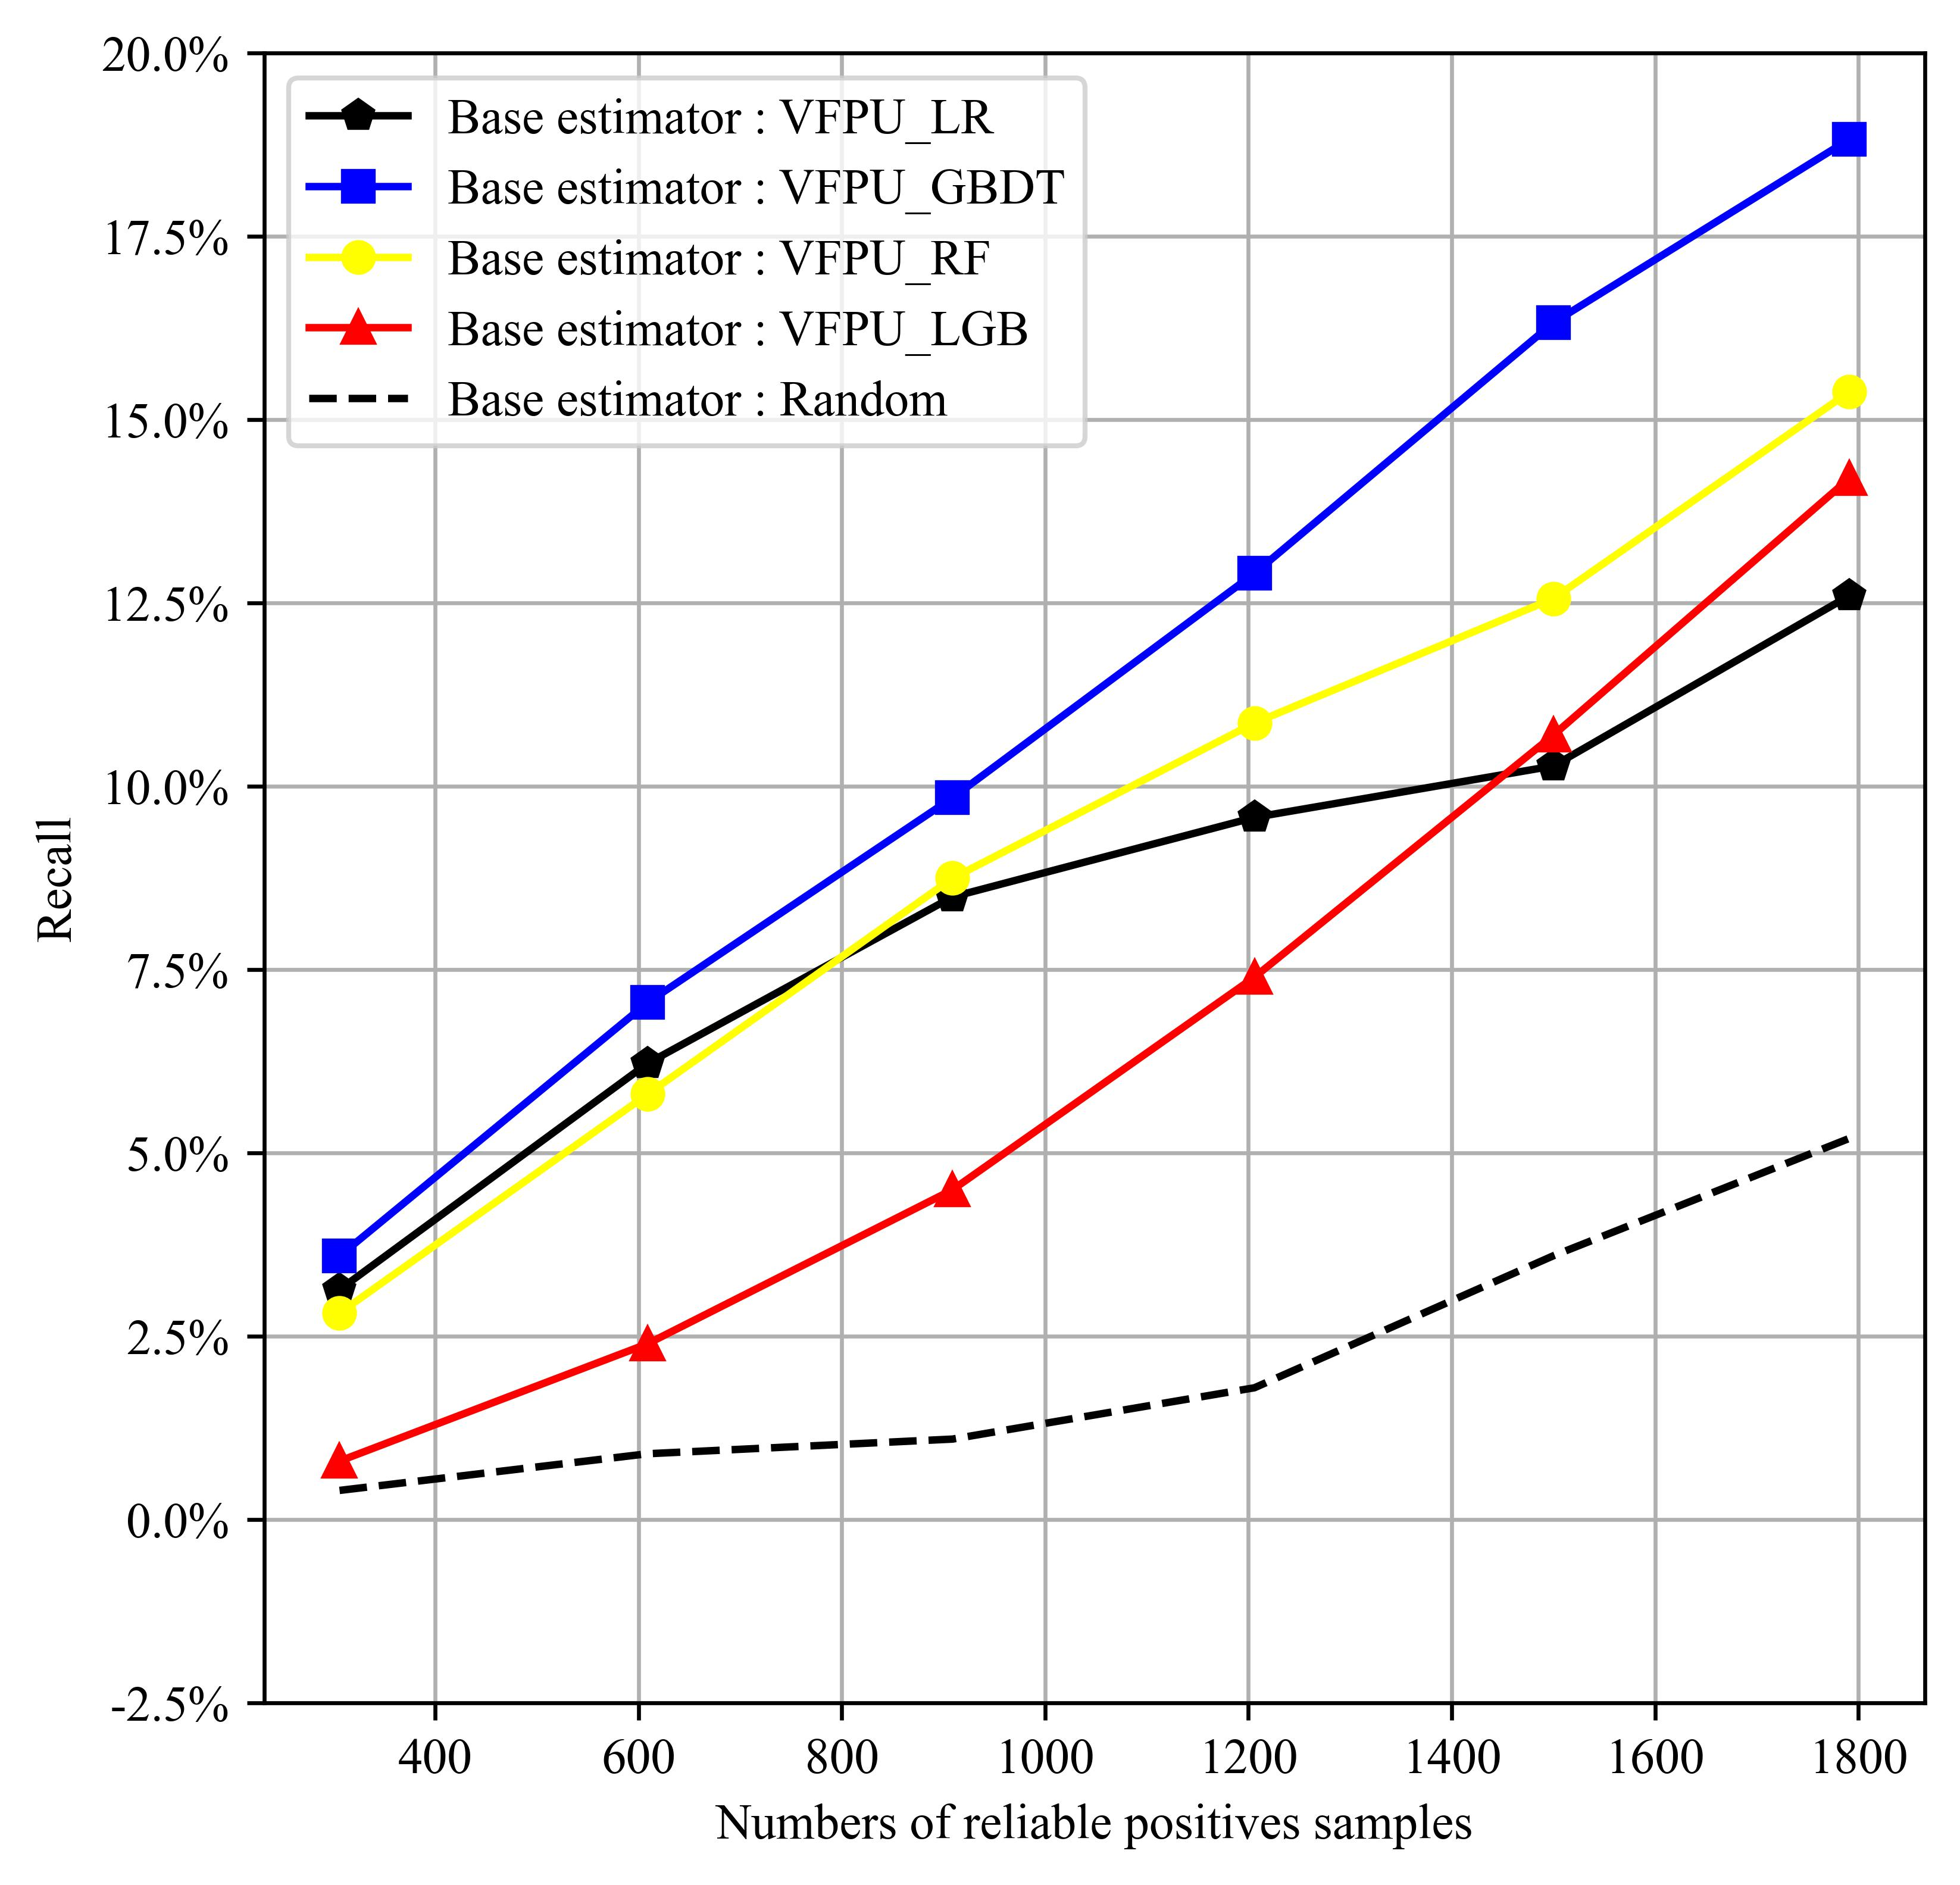
\includegraphics[width=0.45\textwidth,height=4.1cm]{chapters/imgs/Figure 4 (2) in JEPG format}}
	\subfigure[]{\label{RQ2.3.sub3}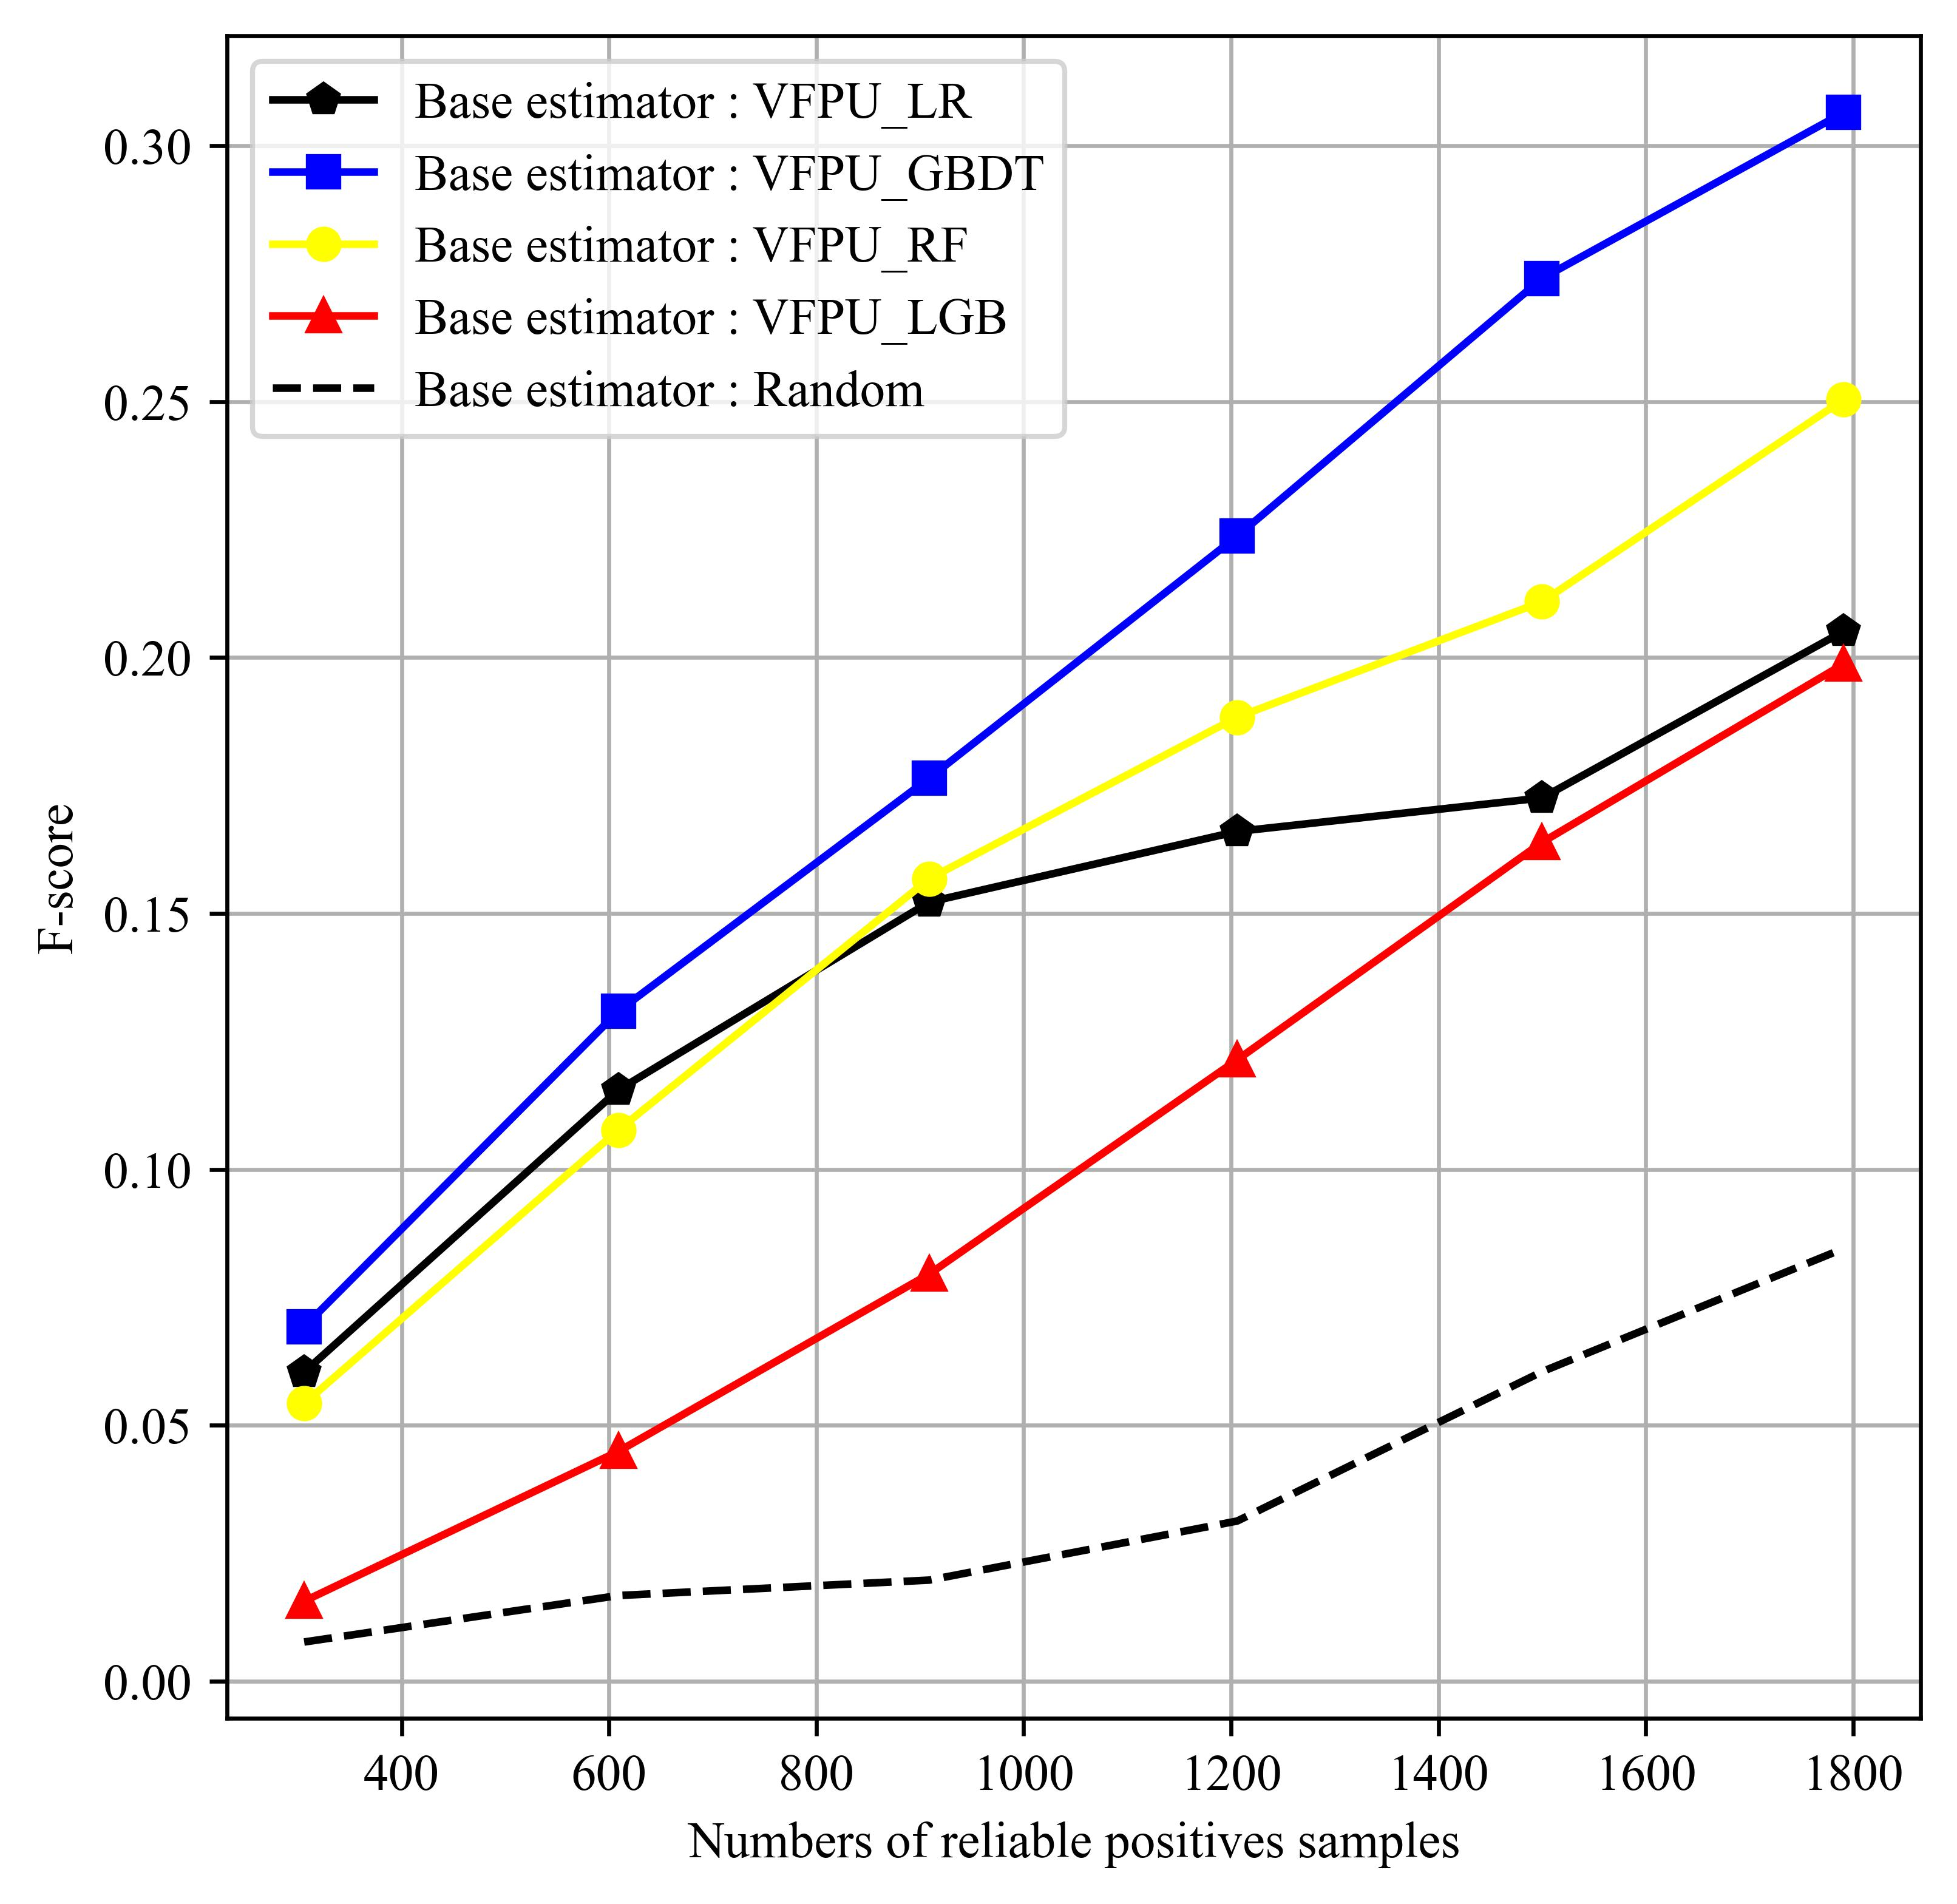
\includegraphics[width=0.45\textwidth,height=4.1cm]{chapters/imgs/Figure 4 (3) in JEPG format}}
	\subfigure[]{\label{RQ2.3.sub4}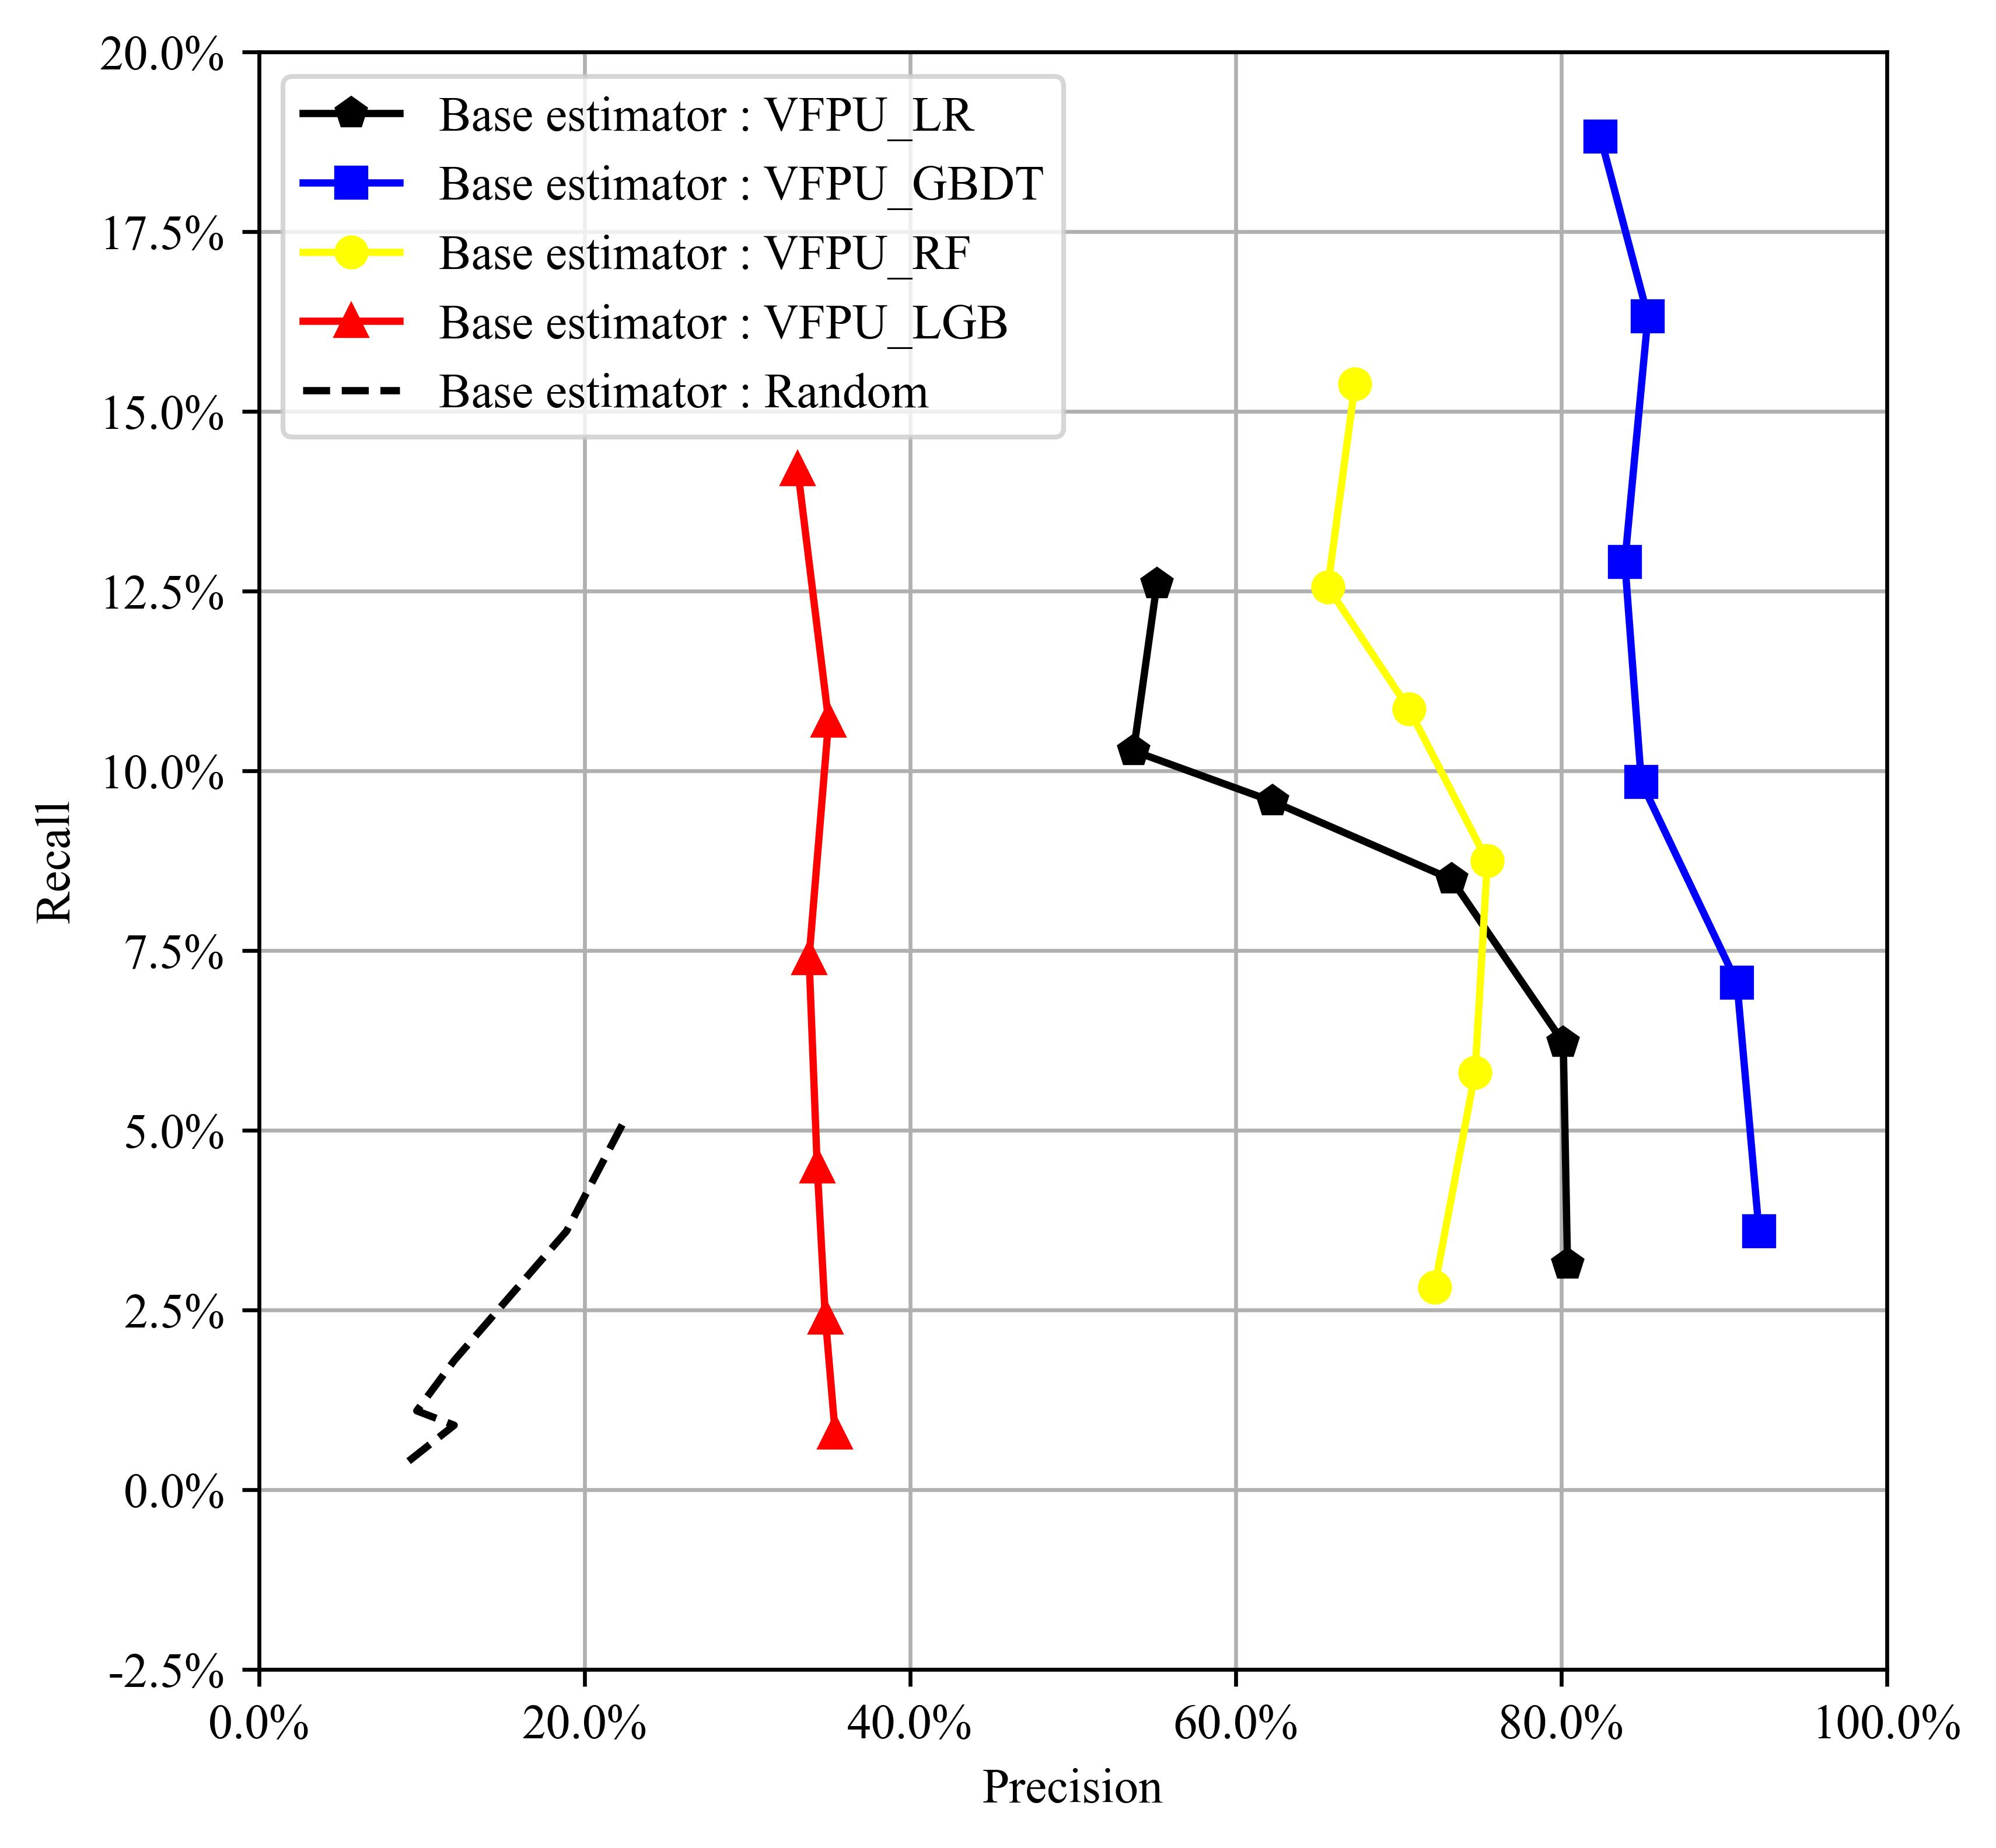
\includegraphics[width=0.45\textwidth,height=4.1cm]{chapters/imgs/Figure 4 (4) in JEPG format}}
	\bicaption[\xiaosi 不同基学器在不同可靠正样本数量下的性能]
	{\centering \songti \wuhao 不同基学器的性能:(a)精度;(b)召回率;(c)F-score;(d)精度-召回率(Census)}
	{\centering \wuhao Base estimators performance: (a) Precision; (b) Recall; (c) F-score; (d) Precision-Recall}
	\label{RQ2.3}
\end{figure}
\vspace{-0.35cm}

此外,图 \ref{RQ2.1.sub4} 中的精确度-召回率曲线进一步验证了VFPU\_GBDT的鲁棒性。通过在各种阈值设置下绘制精确度对召回率的曲线,该曲线有效地捕捉了分类器的性能动态,特别是在类不平衡是关键问题的场景中。VFPU\_GBDT曲线更接近图的右上象限,表明其在多个阈值下的强大性能——这是不平衡分类任务中高性能模型的标志。

图 \ref{RQ2.2}和 图 \ref{RQ2.3} 提供了VFPU\_GBDT估计器有效性的进一步支持证据。这些图报告了在信用卡违约和成人普查数据集上进行的类似实验。尽管数据集在内在特性和分布属性上有所不同,但这些情况下的实验结果反映了与图 \ref{RQ2.1} 中观察到的相似趋势。VFPU\_GBDT在不同数据集上的一致优越性增强了其在VFPU框架中作为基估计器时的可靠性和有效性。

总结来说,三个基准数据集上的实验结果一致表明,VFPU\_GBDT优于VFPU\_LR、VFPU\_RF、VFPU\_LGB以及基线随机抽样技术。VFPU\_GBDT的优越性能,表现为更高的精确度、召回率和平衡的F-score,使其成为在解决UDD-PU问题时VFPU算法最可靠和推荐的基估计器。因此,在所有后续实验中,采用GBDT作为VFPU方法的基估计器,利用其在挑战性条件下实现准确和平衡分类的明显优势。

实验三:基线对比实验,表 \ref{RQ3.1} 显示,提出的No\_Fed\_VFPU\_GBDT方法在所有测试数据集上以及对于各个不同的$num$值均持续优于其他九种半监督方法。例如,在Census数据集中,当$num=1000$时,的方法实现了最高的推荐准确率99\%。这一显著性能与基线方法形成了鲜明对比:\_GBDT、2Step\_GBDT和Bagging\_GBDT分别仅达到64\%、62\%和55\%的准确率。同时,基于深度学习的方法——MixMatch、FixMatch、CoMatch、AdaMatch和SoftMatch——的推荐准确率明显较低,分别为35.94\%、37.06\%、33.39\%、37.28\%和35.86\%。
\vspace{-0.1cm}
\begin{table}[h]
	\centering
	\renewcommand{\arraystretch}{1.2}
	\bicaption[\xiaosi 不同半监督方法的准确推荐百分比(无联邦)]{\wuhao 不同半监督方法的准确推荐百分比(无联邦)}{\wuhao Accurate recommendations  of semi-supervised methods (non-federated)}
	\label{RQ3.1}
	\resizebox{\textwidth}{!}{
		%		{\songti \wuhao
			\begin{tblr}{
					cells = {c},
					cell{1}{1} = {c=2}{},
					cell{2}{1} = {r=10}{},
					cell{12}{1} = {r=10}{},
					cell{22}{1} = {r=10}{},
					hline{1,32} = {-}{1.5pt},    % Top and bottom lines 1.5pt thick
					hline{2,12,22} = {-}{0.75pt} % Middle lines 0.75pt thick
				}
				\diagbox{Datasets \& Methods}{$num$} &                     & 100              & 700              & 1300             & 1900             & 2100             & 2400             \\
				Bank               & MixMatch            & 32.81\%          & 31.25\%          & 24.85\%          & 20.31\%          & 13.44\%          & 12.03\%          \\
				& FixMatch            & 27.81\%          & 25.47\%          & 24.07\%          & 13.28\%          & 12.66\%          & 12.50\%          \\
				& CoMatch             & 31.56\%          & 24.85\%          & 24.07\%          & 17.19\%          & 12.50\%          & 12.03\%          \\
				& AdaMatch            & 33.56\%          & 30.50\%          & 25.78\%          & 20.63\%          & 18.13\%          & 17.19\%          \\
				& SoftMatch           & 32.81\%          & 31.56\%          & 24.53\%          & 19.38\%          & 17.19\%          & 12.50\%          \\
				& \_GBDT              & 53.65\%          & 47.00\%          & 33.62\%          & 28.99\%          & 29.17\%          & 29.33\%          \\
				& Bagging\_GBDT       & 42.74\%          & 33.46\%          & 28.22\%          & 31.67\%          & 27.03\%          & 26.00\%          \\
				& 2Step\_GBDT         & 49.79\%          & 42.79\%          & 29.72\%          & 33.38\%          & 31.30\%          & 26.85\%          \\
				& Pseudo-Labelling    & 33.30\%          & 22.00\%          & 21.80\%          & 24.10\%          & 23.00\%          & 22.70\%          \\
				& No\_Fed\_VFPU\_GBDT & \textbf{77.00\%} & \textbf{66.86\%} & \textbf{59.62\%} & \textbf{54.26\%} & \textbf{53.95\%} & \textbf{52.38\%} \\
				Credit             & MixMatch            & 29.29\%          & 25.34\%          & 24.09\%          & 23.88\%          & 23.47\%          & 21.18\%          \\
				& FixMatch            & 27.00\%          & 25.34\%          & 23.88\%          & 22.85\%          & 22.43\%          & 21.39\%          \\
				& CoMatch             & 26.79\%          & 25.55\%          & 24.09\%          & 23.47\%          & 22.85\%          & 21.18\%          \\
				& AdaMatch            & 26.79\%          & 25.34\%          & 25.13\%          & 22.85\%          & 22.63\%          & 21.18\%          \\
				& SoftMatch           & 26.38\%          & 24.09\%          & 23.47\%          & 22.43\%          & 21.18\%          & 20.97\%          \\
				& \_GBDT              & 42.80\%          & 34.62\%          & 31.56\%          & 29.89\%          & 28.65\%          & 25.43\%          \\
				& Bagging\_GBDT       & 42.74\%          & 30.40\%          & 25.52\%          & 26.17\%          & 26.91\%          & 24.55\%          \\
				& 2Step\_GBDT         & 42.74\%          & 33.29\%          & 31.77\%          & 26.24\%          & 27.57\%          & 26.00\%          \\
				& Pseudo-Labelling    & 38.40\%          & 32.50\%          & 30.90\%          & 29.20\%          & 28.40\%          & 27.30\%          \\
				& No\_Fed\_VFPU\_GBDT & \textbf{51.25\%} & \textbf{50.14\%} & \textbf{47.69\%} & \textbf{41.82\%} & \textbf{40.82\%} & \textbf{39.82\%} \\
				Census             & MixMatch            & 37.72\%          & 36.39\%          & 36.05\%          & 34.15\%          & 32.81\%          & 32.59\%          \\
				& FixMatch            & 38.84\%          & 37.28\%          & 36.39\%          & 34.38\%          & 33.93\%          & 32.36\%          \\
				& CoMatch             & 37.18\%          & 34.06\%          & 32.97\%          & 31.38\%          & 31.38\%          & 31.38\%          \\
				& AdaMatch            & 38.39\%          & 37.50\%          & 36.24\%          & 35.49\%          & 34.38\%          & 33.93\%          \\
				& SoftMatch           & 38.84\%          & 35.94\%          & 35.04\%          & 33.93\%          & 32.81\%          & 29.91\%          \\
				& \_GBDT              & 64.00\%          & 61.00\%          & 58.00\%          & 54.00\%          & 51.00\%          & 54.00\%          \\
				& Bagging\_GBDT       & 68.00\%          & 59.00\%          & 54.00\%          & 52.00\%          & 48.00\%          & 51.00\%          \\
				& 2Step\_GBDT         & 66.00\%          & 63.00\%          & 56.00\%          & 51.00\%          & 52.00\%          & 53.00\%          \\
				& Pseudo-Labelling    & 42.90\%          & 29.30\%          & 28.40\%          & 41.40\%          & 37.30\%          & 45.30\%          \\
				& No\_Fed\_VFPU\_GBDT & \textbf{99.00\%} & \textbf{99.43\%} & \textbf{94.57\%} & \textbf{84.08\%} & \textbf{80.08\%} & \textbf{75.08\%} 
			\end{tblr}
			%		}	
	}
\end{table}
\vspace{-0.5cm}
Match系列算法尽管是半监督学习领域最新的进展,但表现不佳可以归因于两个关键因素。首先,这些方法本质上需要大量标记数据,涵盖正类和负类。然而,在PU问题情境下,负样本并未被明确标记,这使得这些算法处于明显的不利地位。其次,使用Wide ResNet-28模型这一相对复杂的深度学习网络,在面对类分布极度不平衡的数据集时,可能无意中导致过拟合。这种过拟合会削弱模型的泛化能力,从而导致整体性能较低。

相比之下,PU学习方法,包括VFPU\_GBDT、\_GBDT、Bagging\_GBDT和2Step\_GBDT,专门为解决在主要由未标记样本构成的数据集中揭示隐藏正样本这一挑战而设计。这些方法利用数据的内在结构,并采用定制的策略来迭代细化对潜在正实例的识别。因此,如表 \ref{RQ3.1}所示,表现最好的四种方法分别为\_GBDT、Bagging\_GBDT、2Step\_GBDT和VFPU\_GBDT。它们的出色性能突显了PU学习策略在负样本不可直接获得且数据存在显著不平衡的情景中的有效性。

通过对打分机制、超参数设置以及底层模型架构的详细讨论,丰富了分析内容,从而全面理解了实验设置及各方法的相对优劣。这一详细论述凸显了提出的No\_Fed\_VFPU\_GBDT方法在有效揭示隐藏正样本方面的优势,为未来在常规PU学习和联邦PU学习框架下的研究提供了宝贵的启示。

\vspace{-0.1cm}
\begin{table}[h]
	\centering
	\bicaption[\xiaosi 不同半监督方法的准确推荐百分比(纵向联邦)]
	{\wuhao 不同半监督方法的准确推荐百分比(纵向联邦)}
	{\wuhao Accurate recommendations  of semi-supervised methods (in VFL)}
	\label{RQ3.2}
	\resizebox{\textwidth}{!}{
		% 整体使用 {\songti \wuhao ...} 包裹表格内容
		{\songti \wuhao
			\begin{tblr}{
					column{1} = {c},
					column{2} = {c},
					cell{1}{1} = {c=2}{},
					cell{2}{1} = {r=4}{},
					cell{6}{1} = {r=4}{},
					cell{10}{1} = {r=4}{},
					hline{1} = {-}{1.5pt}, % 顶部粗线
					hline{2} = {-}{}, % 表头下方普通线
					hline{6,10} = {-}{}, % 数据区域中的普通横线
					hline{14} = {-}{1.5pt}, % 底部粗线
				}
				\diagbox{Datasets \& Methods}{$num$} &                  & 100              & 700              & 1300             & 1900             & 2100             & 2400             & runtime(s)        \\
				Bank               & VF\_GBDT         & 7.00\%           & 5.30\%           & 4.70\%           & 5.10\%           & 5.00\%           & 4.80\%           & 10673.81          \\
				& VF\_Bagging GBDT & 17.00\%          & 18.90\%          & 19.70\%          & 20.30\%          & 20.70\%          & 20.80\%          & 15069.88          \\
				& VF\_2Step GBDT   & 4.00\%           & 3.60\%           & 5.30\%           & 5.40\%           & 6.50\%           & 7.40\%           & 44030.4           \\
				& VFPU\_GBDT       & \textbf{74.00\%} & \textbf{63.10\%} & \textbf{59.00\%} & \textbf{54.20\%} & \textbf{53.20\%} & \textbf{52.30\%} & \textbf{106922.2} \\
				Credit             & VF\_GBDT         & 18.00\%          & 22.60\%          & 22.10\%          & 21.40\%          & 21.60\%          & 22.30\%          & 12025.47          \\
				& VF Bagging GBDT  & 32.00\%          & 23.90\%          & 23.50\%          & 23.30\%          & 22.30\%          & 22.00\%          & 15791.59          \\
				& VF\_2Step GBDT   & 24.00\%          & 25.40\%          & 23.70\%          & 22.30\%          & 22.30\%          & 22.00\%          & 46954.19          \\
				& VFPU\_GBDT       & \textbf{44.00\%} & \textbf{48.86\%} & \textbf{44.85\%} & \textbf{39.47\%} & \textbf{38.33\%} & \textbf{37.43\%} & \textbf{107075.9} \\
				Census             & VF\_GBDT         & 19.00\%          & 25.40\%          & 23.90\%          & 23.10\%          & 22.90\%          & 22.80\%          & 11581.47          \\
				& VF\_Bagging GBDT & 13.00\%          & 19.90\%          & 22.30\%          & 23.20\%          & 23.20\%          & 23.90\%          & 15987.59          \\
				& VF\_2Step GBDT   & 25.00\%          & 23.10\%          & 24.30\%          & 24.60\%          & 25.00\%          & 25.60\%          & 46808.19          \\
				& VFPU\_GBDT       & \textbf{98.00\%} & \textbf{98.71\%} & \textbf{94.23\%} & \textbf{80.53\%} & \textbf{76.05\%} & \textbf{72.74\%} & \textbf{107089.9} 
			\end{tblr}
		}
	}
\end{table}
\vspace{-0.3cm}

在第二个实验中,将第一个实验中表现最佳的四种方法适配到纵向联邦学习(VFL)环境中,分别标记为VF\_GBDT、VF\_Bagging\_GBDT、VF\_2Step\_GBDT和VFPU\_GBDT。此外,为了评估这些方法在VFL环境中部署时的时间复杂度和计算开销,在$num = 2400$的各种数据集上仔细记录了每种方法的训练时间。训练时间表示为runtime(s),其中s代表秒,详细内容见表 \ref{RQ3.2}。

表 \ref{RQ3.2} 与表 \ref{RQ3.1} 类似,展示了VFL设置下不同方法所达到的准确率百分比的比较分析。结果清晰地表明,VFPU\_GBDT方法在推荐准确率方面始终优于其他三种方法。例如,在Census数据集上,当$num=1000$时,VFPU\_GBDT达到了显著高的98.70\%的推荐准确率,这明显高于VF\_GBDT、VF\_Bagging\_GBDT和VF\_2Step\_GBDT的准确率,它们分别为24.20\%、21.10\%和24.30\%。在Credit数据集上,尽管VFPU\_GBDT展示了更高的准确率,但它带来了更高的计算成本:本章的方法记录的运行时间为107075.9s,而VF\_GBDT、VF\_Bagging\_GBDT和VF\_2Step\_GBDT的运行时间分别为12025.47s、15791.59s和46954.19s。

值得注意的是,按runtime(s)指标衡量,VFPU\_GBDT的耗时约为其他方法的10倍。这种增加的时间消耗主要是由于VFPU\_GBDT在选择可靠正样本时采用了更为谨慎和迭代的策略。该算法采用多次迭代,每次迭代只选择一小部分样本,确保只有最可靠和准确预测的正样本被选中。这种谨慎的选择过程引入了额外的计算开销。然而,这种训练时间与推荐准确率之间的权衡被认为是可接受的,因为准确率的显著提高证明了额外训练时间的合理性。


\vspace{-0.1cm}
\begin{figure}[h]
	\centering 
	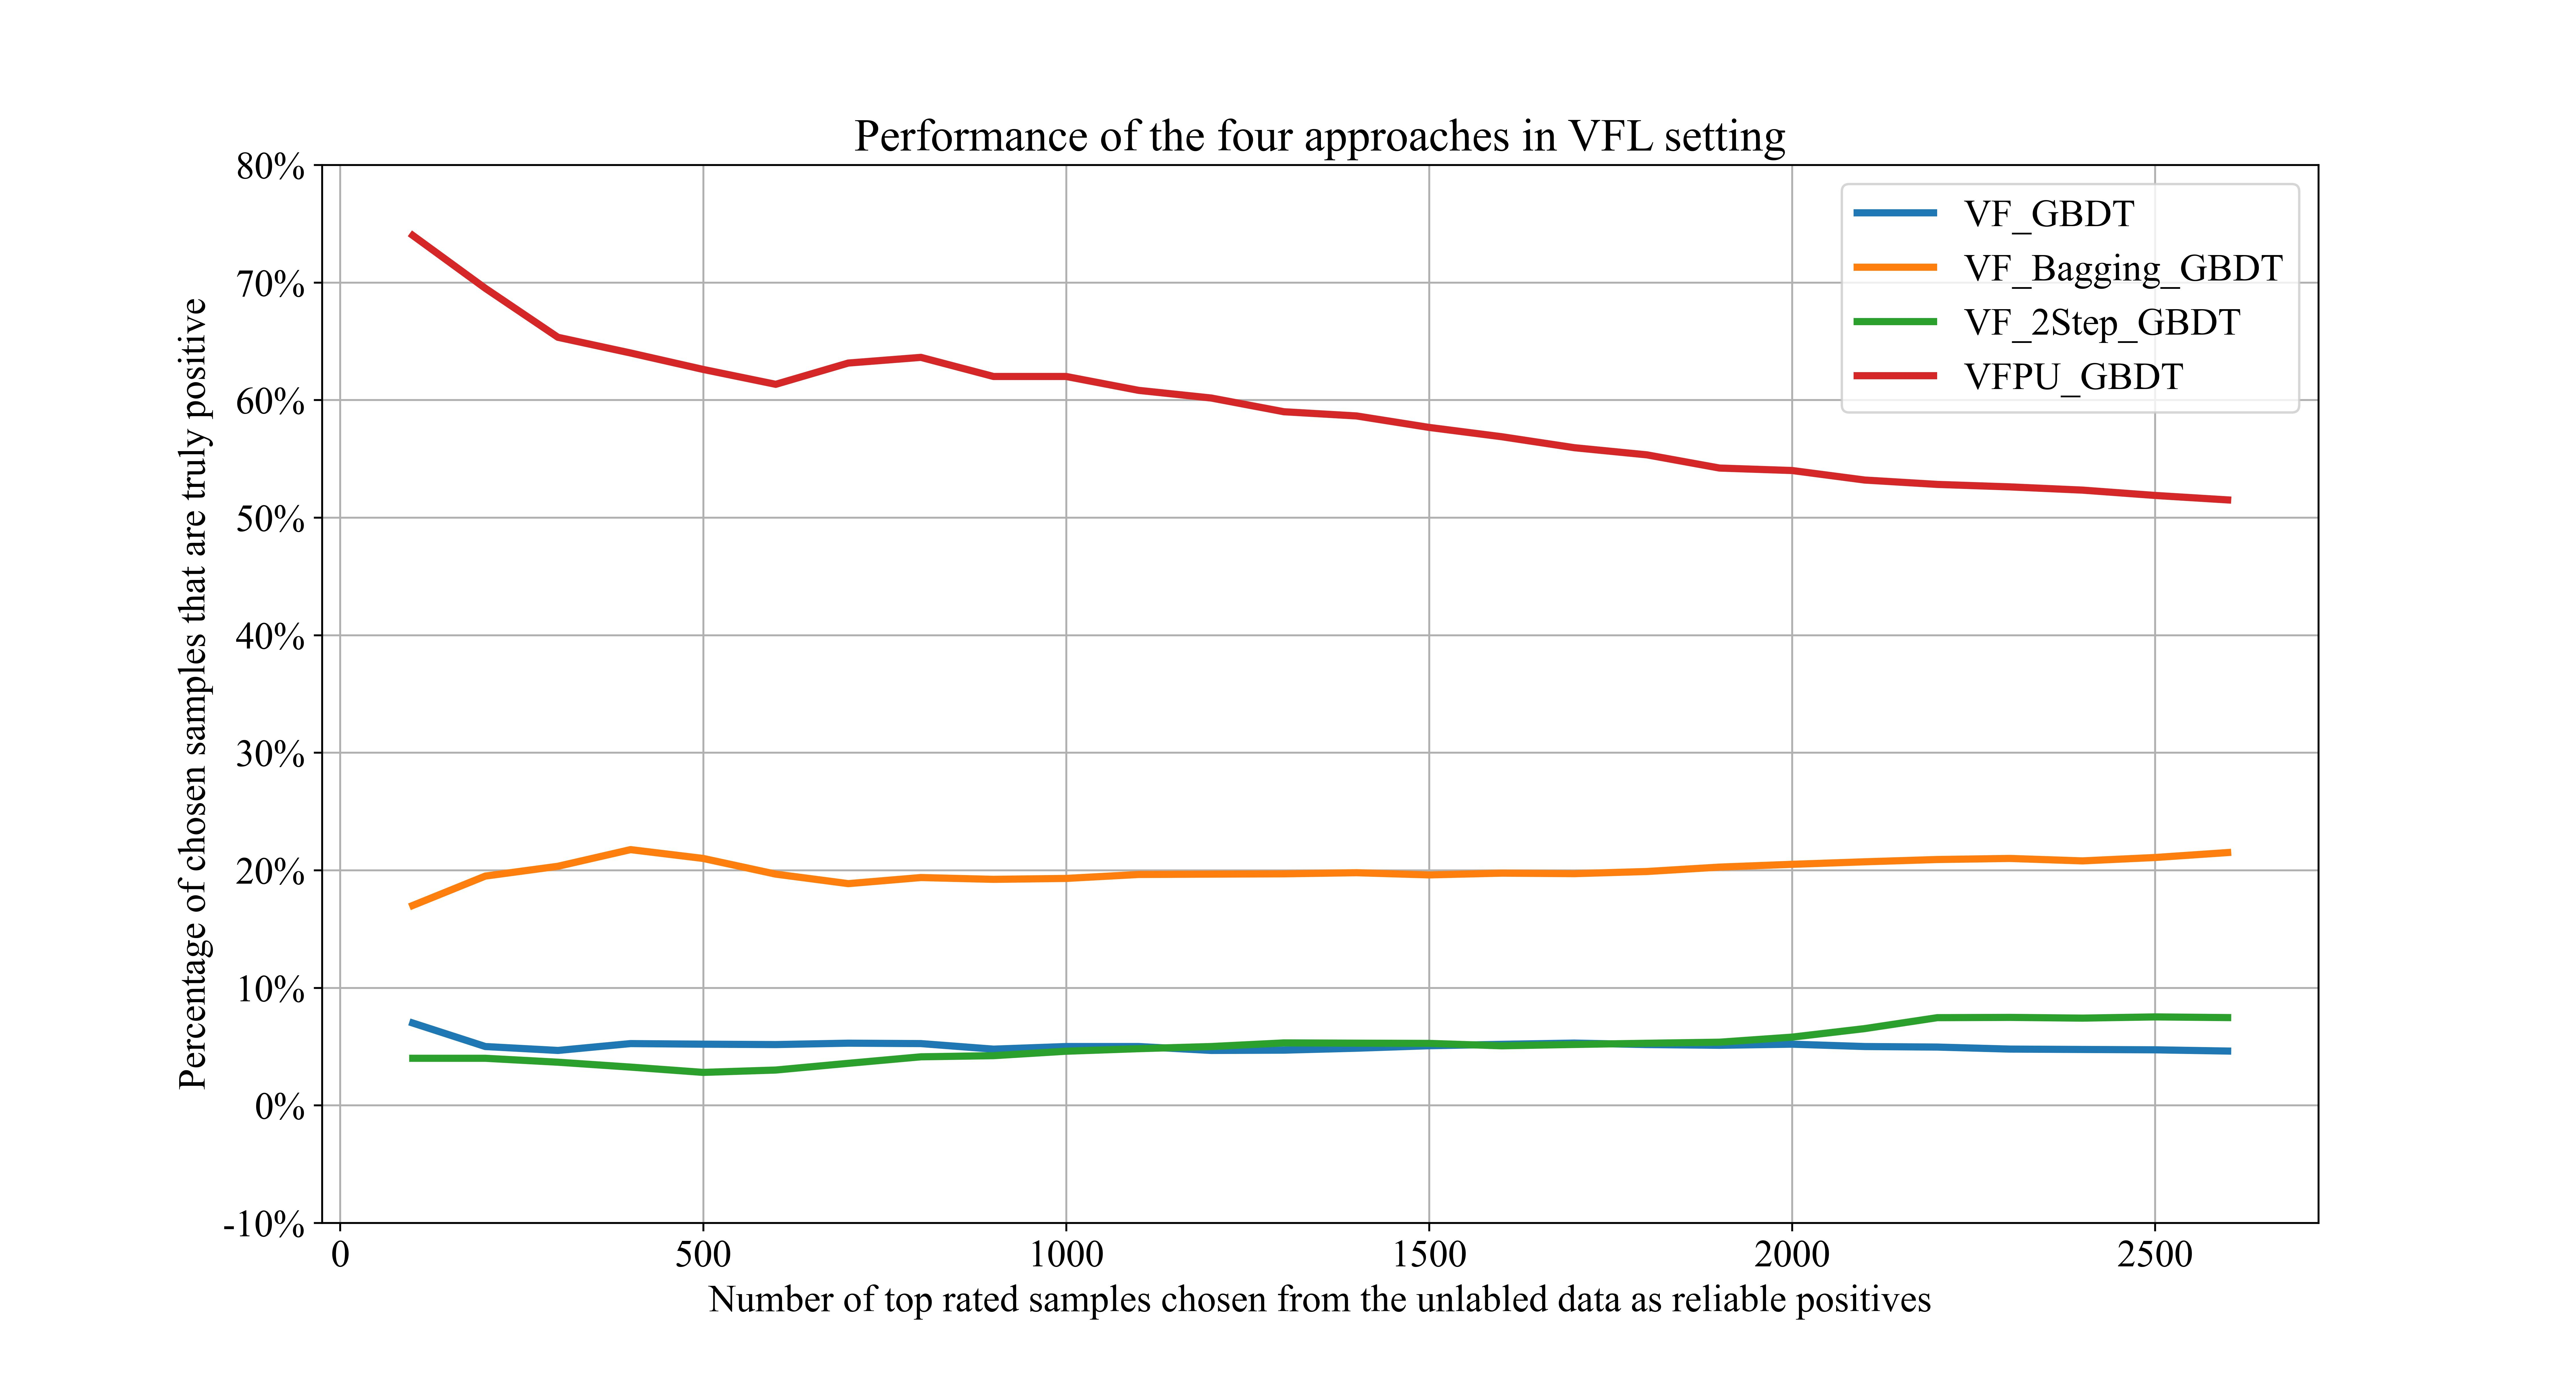
\includegraphics[width=0.9\textwidth]{chapters/imgs/Figure 5 in JPEG format}
	\bicaption[\xiaosi 不同半监督方法在纵向联邦学习(VFL)中的准确推荐百分比]
	{\centering \wuhao 不同半监督方法在纵向联邦学习(VFL)中的准确推荐百分比(Bamk 数据集)}
	{\centering \wuhao The accurate recommendations percentage by Different Semi-supervised Methods in VFL (The Bank Marketing Dataset)}
	\label{fig:GBDT}
\end{figure}
\vspace{-0.35cm}

图  \ref{fig:GBDT} 提供了表 \ref{RQ3.2} 中讨论的银行营销数据集实验结果的可视化表示。在该图中,x轴表示被选为可靠正样本的评分最高的未标记样本数量,而y轴表示这些被选择样本中真正为正样本的百分比。图中清晰地说明,随着$num$从100增加到1000,VFPU\_GBDT识别的隐藏正样本数量迅速减少。这种观察到的减少可归因于几个因素。最初,与正类表现出强烈相似性或与负类有明显差异的未标记数据样本被迅速识别和选择。然而,随着选择过程的继续,剩余的未标记数据往往在正负类之间表现出特征重叠,这给分类器带来干扰。这种干扰导致错误分类,从而降低了准确推荐的百分比。虽然其他方法在不同$num$值下表现相对稳定,但这种表面上的稳定性并不一定是有利的。这些方法始终较低的准确推荐百分比表明它们在可靠识别隐藏正样本方面能力有限。此外,考虑到未标记数据集中只有约2500个真正的正样本,当选择的正样本数量超过这个阈值时,VFPU\_GBDT的准确率自然会下降。

总之,实验结果提供了强有力的证据,表明VFPU\_GBDT算法在VFL环境中推荐可靠正样本方面非常有效。尽管需要额外的计算时间,但推荐准确率的显著提升使VFPU\_GBDT相比其他半监督方法成为更优方案。这项实验突显了在联邦学习环境中应用VFPU\_GBDT算法解决未标记数据缺乏的PU(UDD-PU)学习推荐问题的显著优势,强调了它在高准确率至关重要的实际应用中的潜力。

\section{本章小结}
本章主要介绍了未标记数据缺乏的PU(UDD-PU)学习问题,其中需要模型训练的一方仅持有正样本数据,而其他参与方拥有大量未标记数据。为解决UDD-PU问题,本章提出了一种基于半监督学习的多方联邦推荐方法。具体而言,设计了VFPU算法作为该方法的核心,该算法有效整合了两种PU学习技术,并将其适配到纵向联邦学习框架中。通过这种方式,VFPU能够利用有限的标记数据(正样本)和丰富的未标记数据来提高推荐模型的性能。在三个数据集上评估了所提出的方法,并将其与其他半监督学习方法进行了比较。实验结果明确表明,VFPU算法在确保数据隐私的同时,与非联邦方法相比只有很小的性能下降,就能达到令人满意的性能。此外,证明了VFPU算法在纵向联邦学习环境中发现隐藏正样本方面始终优于其他半监督学习方法。而且,对不同基学习器的分析表明,梯度提升决策树(VFPU\_GBDT)在精确率、召回率和F值方面持续展现出卓越的性能。这一发现强调了为VFPU算法选择适当基学习器的重要性,以便在各种实际应用中优化其性能。

% 第4章


\chapter{总结与展望}
\thispagestyle{others}
\pagestyle{others}
\xiaosi

\section{主要结论}

本文主要……

\section{研究展望}

更深入的研究……

以下文字用于测试。

以下文字用于测试。

以下文字用于测试。

以下文字用于测试。

以下文字用于测试。

以下文字用于测试。

以下文字用于测试。

以下文字用于测试。

以下文字用于测试。

以下文字用于测试。

以下文字用于测试。

以下文字用于测试。

以下文字用于测试。

以下文字用于测试。

以下文字用于测试。

以下文字用于测试。

以下文字用于测试。

以下文字用于测试。

以下文字用于测试。

以下文字用于测试。

以下文字用于测试。

以下文字用于测试。

以下文字用于测试。

以下文字用于测试。

以下文字用于测试。

以下文字用于测试。

以下文字用于测试。

以下文字用于测试。




%如果要增加章节数请在此加项

\backmatter

%取消后续章节的页眉上的章节编号
\renewcommand{\chaptermark}[1]{\markboth{#1}{}}

%参考文献
\begin{thebibliography}{200}
	\wuhao %设置参考文献字体大小
	\linespread{1}\selectfont
	\setlength{\itemsep}{-1.4ex} %缩小条目间行距
	\thispagestyle{others}
	\pagestyle{others}
	
	\makeatletter
	\renewcommand\@biblabel[1]{[#1]\hfill} %序号左对齐
	\makeatother
	\setlength{\labelsep}{0cm}
	
	
	\bibitem{chen2021secureboost+}
	FAN, CHEN, MA et al. SecureBoost+: Large Scale and\&nbsp;High-Performance Vertical Federated Gradient Boosting Decision Tree[C]. Advances in Knowledge Discovery and Data Mining: 28th Pacific-Asia Conference on Knowledge Discovery and Data Mining, PAKDD 2024, Taipei, Taiwan, May 7–10, 2024, Proceedings, Part III, Berlin, Heidelberg, 2024: 237–249.
	
	\bibitem{de2010practical}
	CRISTOFARO D, TSUDIK, GENE. Practical Private Set Intersection Protocols with Linear Complexity[C]. Financial Cryptography and Data Security: 14th International Conference, FC 2010, Tenerife, Canary Islands, January 25-28, 2010, Revised Selected Papers 14, Berlin, Heidelberg, 2010: 143-159.
	
	\bibitem{li2021comatch}
	HOI SCH. CoMatch: Semi-Supervised Learning with Contrastive Graph Regularization[C]. Proceedings of the IEEE/CVF International Conference on Computer Vision (ICCV), Los Alamitos, CA, USA, 2021: 9475-9484.
	
	\bibitem{jin2023federated}
	TSOUVALAS, SAEED, OZCELEBI et al. Labeling Chaos to Learning Harmony: Federated Learning with Noisy Labels[J]. ACM Trans. Intell. Syst. Technol., 2024, 15(2): 26.
	
	\bibitem{liang2022rscfed}
	LIANG, LIN, FU et al. RSCFed: Random Sampling Consensus Federated Semi-Supervised Learning[C]. Proceedings of the IEEE/CVF Conference on Computer Vision and Pattern Recognition, New Orleans, LA, USA, 2022: 10154-10163.
	
	\bibitem{tarvainen2017mean}
	TARVAINEN, VALPOLA, HARRI. Mean teachers are better role models: Weight-averaged consistency targets improve semi-supervised deep learning results[C]. Advances in Neural Information Processing Systems, Red Hook, NY, USA, 2017: 1195-1204.
	
	\bibitem{fan2022private}
	FAN, HU, HUANG et al. Private Semi-Supervised Federated Learning[C]. Proceedings of the Thirty-First International Joint Conference on Artificial Intelligence, Vienna, Austria, 2022: 2009-2015.
	
	\bibitem{jeong2020federated}
	ZHENG, TANG, JU et al. 2024 IEEE International Conference on Bioinformatics and Biomedicine (BIBM)[C]. 2024 IEEE International Conference on Bioinformatics and Biomedicine (BIBM), 2024: 4054-4059.
	
	\bibitem{lin2022federated}
	LIN, CHEN, XU et al. Federated Learning with Positive and Unlabeled Data[C]. International Conference on Machine Learning, Baltimore, MD, USA, 2022: 13344-13355.
	
	\bibitem{wang2022enhancing}
	WANG, XU, XU et al. Enhancing Federated Learning with In-Cloud Unlabeled Data[C]. 2022 IEEE, Kuala Lumpur, Malaysia, 2022: 136-149.
	
	\bibitem{itahara2021distillation}
	ITAHARA, NISHIO, KODA et al. Distillation-based semi-supervised federated learning for communication-efficient collaborative training with non-iid private data[J]. IEEE Transactions on Mobile Computing, 2021, 22(1): 191-205.
	
	\bibitem{diao2022semifl}
	DIAO, DING, TAROKH et al. Semifl: Semi-supervised federated learning for unlabeled clients with alternate training[C]. Advances in Neural Information Processing Systems, New Orleans, LA, USA, 2022: 17871-17884.
	
	\bibitem{hinton2006reducing}
	HINTON, SALAKHUTDINOV, R. R. Reducing the Dimensionality of Data with Neural Networks[J]. Science, 2006, 313(5786): 504-507.
	
	\bibitem{kingma2013auto}
	CHEN, LIU, PENG et al. Auto-encoding variational Bayes[J]. Cambridge Explorations in Arts and Sciences, 2024, 2(1).
	
	\bibitem{xu2019modeling}
	XU, SKOULARIDOU, CUESTA-INFANTE et al. Modeling Tabular Data Using Conditional GAN[C]. Advances in Neural Information Processing Systems, Vancouver, Canada, 2019: 7333-7343.
	
	\bibitem{goodfellow2014generative}
	GOODFELLOW, POUGET-ABADIE, MIRZA et al. Generative Adversarial Nets[C]. Advances in Neural Information Processing Systems, Montreal, Canada, 2014: 2672-2680.
	
	\bibitem{mirza2014conditional}
	MIRZA, OSINDERO, SIMON. Conditional Generative Adversarial Nets[J]. Computer Science, 2014: 2672-2680.
	
	\bibitem{adler2018banach}
	ADLER, LUNZ, SEBASTIAN. Banach Wasserstein[C]. Advances in Neural Information Processing Systems, La Jolla, CA, USA, 2018: 6754-6763.
	
	\bibitem{arjovsky2017towards}
	BOTTOU L. Towards Principled Methods for Training Generative Adversarial Networks[C]. International Conference on Learning Representations, Toulon, France, 2017.
	
	\bibitem{xu2018synthesizing}
	LIU, FAN, LI et al. Tabular data synthesis with generative adversarial networks: design space and optimizations[J]. The VLDB Journal, 2023, 33(2): 255–280.
	
	\bibitem{lee2021invertible}
	LEE, HYEONG, JEON et al. Invertible Tabular GAN[C]. Advances in Neural Information Processing Systems, Red Hook, NY, USA, 2021: 4263-4273.
	
	\bibitem{nguyen2017dual}
	NGUYEN, LE, VU et al. Dual discriminator generative adversarial nets[C]. Advances in Neural Information Processing Systems, Red Hook, NY, USA, 2017: 2670-2680.
	
	\bibitem{singh2021metgan}
	SINGH, KAYATHWAL, WADHWA et al. Metgan: Memory efficient tabular gan for high cardinality categorical datasets[C]. Neural Information Processing: 28th International Conference, ICONIP 2021, Sanur, Bali, Indonesia, December 8--12, 2021, Proceedings, Part VI, Cham, Switzerland, 2021: 519-527.
	
	\bibitem{zhao2021ctab}
	ZHAO, KUNAR, BIRKE et al. Ctab-gan: Effective table data synthesizing[C]. Asian Conference on Machine Learning, Virtual, 2021: 97-112.
	
	\bibitem{engelmann2021conditional}
	ENGELMANN, LESSMANN, STEFAN. Conditional Wasserstein GAN-based oversampling of tabular data for imbalanced learning[J]. Expert Systems with Applications, 2021, 174: 114582.
	
	\bibitem{ho2020denoising}
	HO, JAIN, ABBEEL et al. Denoising Diffusion Probabilistic Models[C]. Advances in Neural Information Processing Systems, Red Hook, NY, 2020: 6840-6851.
	
	\bibitem{kotelnikov2023tabddpm}
	KOTELNIKOV, BARANCHUK, RUBACHEV et al. TabDDPM: Modelling Tabular Data with Diffusion Models[C]. International Conference on Machine Learning, Honolulu, Hawaii, USA, 2023: 17564-17579.
	
	\bibitem{yang2019federated}
	YANG, LIU, CHEN et al. Federated Machine Learning: Concept and Applications[J]. ACM Transactions on Intelligent Systems and Technology (TIST), 2019, 10(2): 1-19.
	
	\bibitem{mcmahan2017communication}
	MCMAHAN, MOORE, RAMAGE et al. Communication-Efficient Learning of Deep Networks from Decentralized Data[C]. Proceedings of the 20th International Conference on Artificial Intelligence and Statistics AISTATS, Fort Lauderdale, FL, USA, 2017: 1273-1282.
	
	\bibitem{konevcny2016federated}
	KONEVCNY, MCMAHAN, YU et al. Federated Learning: Strategies for Improving Communication Efficiency[J]. arXiv preprint, 2016, abs/1610.05492.
	
	\bibitem{li2020federated}
	LI, SAHU, ZAHEER et al. Federated Optimization in Heterogeneous Networks[J]. Proceedings of Machine Learning and Systems, 2020, 2: 429-450.
	
	\bibitem{kairouz2021advances}
	KAIROUZ, MCMAHAN, AVENT et al. Advances and Open Problems in Federated Learning[J]. Foundations and Trends\textregistered, 2021, 14(1--2): 1-210.
	
	\bibitem{konevcny2015federated}
	LI, LI, ZHANG et al. Federated Adam-Type Algorithm for Distributed Optimization With Lazy Strategy[J]. IEEE Internet of Things Journal, 2022, 9(20): 20519-20531.
	
	\bibitem{liu2019communication}
	LIU, HUANG, LI et al. Communication-efficient federated learning for wireless edge intelligence: A survey[C]. 2019 IEEE 20th International Conference on Communication Technology (ICCT), Xi'an, China, 2019: 1327-1332.
	
	\bibitem{liu2020secure}
	LIU, KANG, XING et al. A secure federated transfer learning framework[J]. IEEE Intelligent Systems, 2020, 35(4): 70-82.
	
	\bibitem{chen2020vafl}
	CHEN, YIN, LI et al. VaFL: A method of vertical asynchronous federated learning for heterogeneous data distribution[C]. 2020 International Conference on Machine Learning and Cybernetics (ICMLC), Adelaide, Australia, 2020: 1-7.
	
	\bibitem{2015Semi}
	RASMUS, VALPOLA, HONKALA et al. Semi-Supervised Learning with Ladder Networks[J]. Computer Science, 2015, 9 Suppl 1(1): 1-9.
	
	\bibitem{van2020survey}
	ENGELEN v, HOOS, H. H. A survey on semi-supervised learning[J]. Machine Learning, 2020, 109(2): 373-440.
	
	\bibitem{lee2013pseudo}
	LEE, DONG-HYUN. Pseudo-label: The simple and efficient semi-supervised learning method for deep neural networks[C]. ICML Workshop on Challenges in Representation Learning, Atlanta, GA, USA, 2013: 896-903.
	
	\bibitem{elkan2008learning}
	ELKAN, NOTO, KEITH. Learning classifiers from only positive and unlabeled data[C]. Proceedings of the 14th ACM, New York, NY, USA, 2008: 213-220.
	
	\bibitem{mordelet2013bagging}
	MORDELET, VERT, JEAN-PHILIPPE. Bagging for positive and unlabeled learning[J]. IEEE Transactions on Pattern Analysis and Machine Intelligence, 2013, 35(10): 2402-2412.
	
	\bibitem{li2021survey}
	LI, ZHANG, CHEN et al. A Survey on Tabular Data Generation Techniques[J]. IEEE Transactions on Knowledge and Data Engineering, 2021, 33(12): 6213-6232.
	
	\bibitem{zhang2020tab}
	ZHANG, WU, DU et al. TAB: A Hybrid Framework for Multi-dimensional Table Synthesis[C]. Proceedings of the Thirty-Fourth AAAI Conference on Artificial Intelligence, New York, NY, USA, 2020: 1234-1241.
	
	\bibitem{brown2019differential}
	BROWN, WILLIAMS, DAVIS et al. Differentially Private Synthetic Tabular Data Generation via Deep Generative Models[C]. Proceedings of the 2019 IEEE International Conference on Data Mining (ICDM), Beijing, China, 2019: 567-576.
	
	\bibitem{hardt2016equality}
	HARDT, PRICE, SREBRO et al. Equality of Opportunity in Supervised Learning[C]. Advances in Neural Information Processing Systems, Red Hook, NY, USA, 2016: 3315-3323.
	
	\bibitem{rudin2019stop}
	RUDIN, CYNTHIA. Stop Explaining Black Box Machine Learning Models for High Stakes Decisions and Use Interpretable Models Instead[J]. Nature Machine Intelligence, 2019, 1(5): 206-215.
	
	\bibitem{esteva2017dermatologist}
	ESTEVA, KUPREL, NOVOA et al. Dermatologist-Level Classification of Skin Cancer with Deep Neural Networks[J]. Nature, 2017, 542(7639): 115-118.
	
	\bibitem{miotto2018deep}
	MIOTTO, WANG, WANG et al. Deep Learning for Healthcare: Review, Opportunities and Challenges[J]. Briefings in Bioinformatics, 2018, 19(6): 1236-1246.
	
	\bibitem{lee2015cyber}
	LEE, BAGHERI, KAO et al. A Cyber-Physical Systems Architecture for Industry 4.0-Based Manufacturing Systems[J]. Manufacturing Letters, 2015, 3(1): 18-23.
	
	\bibitem{tao2018digital}
	TAO, CHENG, QI et al. Digital Twin-Driven Product Design, Manufacturing and Service with Big Data[J]. The International Journal of Advanced Manufacturing Technology, 2018, 94(9): 3563-3576.
	
	\bibitem{wang2019deep}
	WANG, MA, ZHANG et al. Deep Learning for Smart Manufacturing: Methods and Applications[J]. Journal of Manufacturing Systems, 2018, 48: 144-156.
	
	\bibitem{zhang2019short}
	LEE, EO, JUNG et al. Short-term traffic prediction with deep neural networks: A survey[J]. IEEE Access, 2021, 9: 54739-54756.
	
	\bibitem{mordelet2014bagging}
	MORDELET, VERT, J-P. A bagging SVM to learn from positive and unlabeled examples[J]. Pattern Recognition Letters, 2014, 37(1): 201-209.
	
	\bibitem{liu2003building}
	LIU, DAI, LI et al. Building text classifiers using positive and unlabeled examples[C]. Proceedings of the Third IEEE International Conference on Data Mining, Melbourne, FL, USA, 2003: 179-186.
	
	\bibitem{liu2015classification}
	LIU, TAO, DACHENG. Classification with Noisy Labels by Importance Reweighting[J]. IEEE Transactions on Pattern Analysis and Machine Intelligence, 2015, 38(3): 447-461.
	
	\bibitem{xu2017multi}
	XU, XU, XU et al. Multi-Positive and Unlabeled Learning[C]. Proceedings of the 26th International Joint Conference on Artificial Intelligence, Melbourne, Australia, 2017: 3182-3188.
	
	\bibitem{he2021secure}
	HE, DU, ZHU et al. Secure logistic regression for vertical federated learning[J]. IEEE Internet Computing, 2021, 26(2): 61-68.
	
	\bibitem{yang2019parallel}
	LIU SYaBRaXZaL. Parallel Distributed Logistic Regression for Vertical Federated Learning
	without Third-Party Coordinator[J]. Clinical Orthopaedics and Related Research, 2019, abs/1911.09824.
	
	\bibitem{yao2022efficient}
	GENCTURK, SINACI, CICEKLI et al. BOFRF: A novel boosting-based federated random forest algorithm on horizontally partitioned data[J]. IEEE Access, 2022, 10: 89835-89851.
	
	\bibitem{xu2021efficient}
	HAN, CHENG, ZHAO et al. SecureXGB: A Secure and Efficient Multi-party Protocol for Vertical Federated XGBoost[J]. Proc. ACM Manag. Data, 2025, 3(1): 26.
	
	\bibitem{wang2022feverless}
	WANG, ERSOY, OUG. Feverless: Fast and Secure Vertical Federated Learning Based on XGBoost for Decentralized Labels[J]. IEEE Transactions on Big Data, 2022, 9(1): 295-308.
	
	\bibitem{feng2019securegbm}
	FENG, XIONG, SONG et al. Securegbm: Secure multi-party gradient boosting[C]. 2019 IEEE International Conference on Big Data (Big Data), Los Angeles, CA, USA, 2019: 1312-1321.
	
	\bibitem{fitriani2021data}
	FITRIANI, FEBRIANTO, CANDRA D. Data mining for potential customer segmentation in the marketing bank dataset[J]. JUITA: Jurnal Informatika, 2021, 9(1): 25-32.
	
	\bibitem{subasi2019prediction}
	SUBASI, CANKURT, SELCUK. Prediction of default payment of credit card clients using Data Mining Techniques[C]. 2019 International Engineering Conference (IEC), Istanbul, Turkey, 2019: 115-120.
	
	\bibitem{chakrabarty2018statistical}
	CHAKRABARTY, BISWAS, SANKET. A statistical approach to adult census income level prediction[C]. 2018 International Conference on Advances in Computing, Communication Control and Networking (ICACCCN), Greater Noida, India, 2018: 207-212.
	
	\bibitem{aono2016scalable}
	AONO, HAYASHI, PHONG T et al. Scalable and secure logistic regression via homomorphic encryption[C]. Proceedings of the Sixth ACM Conference on Data and Application Security and Privacy, New York, NY, USA, 2016: 142-144.
	
	\bibitem{li2022fedtree}
	LI, ZHAOMIN, CAI et al. Proceedings of Machine Learning and Systems[C]. Proceedings of Machine Learning and Systems, 2023: 89-103.
	
	\bibitem{liu2021fate}
	LIU, FAN, CHEN et al. FATE: An Industrial Grade Platform for Collaborative Learning with Data Protection[J]. Journal of Machine Learning Research, 2021, 22(226): 1-27.
	
	\bibitem{chen2015xgboost}
	CHEN, HE, BENESTY et al. Xgboost: extreme gradient boosting[J]. R package version 0.4-2, 2015, 1(4): 1-4.
	
	\bibitem{ke2017lightgbm}
	KE, MENG, FINLEY et al. Lightgbm: A highly efficient gradient boosting decision tree[C]. Advances in Neural Information Processing Systems, Red Hook, NY, USA, 2017: 3146-3154.
	
	\bibitem{pedregosa2011scikit}
	PEDREGOSA, VAROQUAUX, GA\"E. Scikit-learn: Machine Learning in P[J]. Journal of Machine Learning Research, 2011, 12: 2825-2830.
	
	\bibitem{paillier1999public}
	PAILLIER, PASCAL. Public-Key Cryptosystems Based on Composite Degree Residuosity Classes[C]. Advances in Cryptology---EUROCRYPT '99, Berlin, Heidelberg, 1999: 223-238.
	
	\bibitem{cheng2021secureboost}
	CHENG, FAN, JIN et al. Secureboost: A Lossless Federated Learning Framework[J]. IEEE Intelligent Systems, 2021, 36(6): 87-98.
	
	\bibitem{sohn2020fixmatch}
	SOHN, BERTHELOT, LI et al. FixMatch: simplifying semi-supervised learning with consistency and confidence[C]. Proceedings of the 34th International Conference on Neural Information Processing Systems, Red Hook, NY, USA, 2020: 13.
	
	\bibitem{oliver2018realistic}
	OLIVER, ODENA, RAFFEL et al. Realistic evaluation of deep semi-supervised learning algorithms[C]. Proceedings of the 32nd International Conference on Neural Information Processing Systems, Red Hook, NY, USA, 2018: 3239–3250.
	
	\bibitem{liu2023multi}
	LIU, LV, CHEN et al. Multi-Party Federated Recommendation Based on Semi-Supervised Learning[J]. IEEE Transactions on Big Data, 2023, 10(4): 356-370.
	
\end{thebibliography}
\clearpage



%如果没有附录请自行删除以下页面

%附录A
%\specialsectioning
\chapter{附录A 各学院中英文名称对照表}
\thispagestyle{others}

\begin{table}[h]
	\renewcommand{\arraystretch}{1.5}
	\centering
	\begin{tabular}{p{2cm}p{3cm}p{8.5cm}}
		\toprule[1.5pt]
		\makecell[c]{\songti\xiaosi\bfseries 序号}&\makecell[l]{\songti\xiaosi\bfseries 中文名称}&\makecell[l]{\songti\xiaosi\bfseries 英文名称}\\
		\hline
		\makecell[c]{\wuhao 01}&\makecell[l]{\wuhao 通信工程学院}&\makecell[c]{\wuhao School of Communications and Information Engineering}\\
		\bottomrule[1.5pt]
	\end{tabular}
	
\end{table}

\clearpage

%附录B
%%\specialsectioning
\chapter{附录B 常见一级学科中英文名称对照表}
\thispagestyle{others}



\begin{table}[h]
	\renewcommand{\arraystretch}{1.5}
	\centering
	\begin{tabular}{p{2cm}p{3cm}p{8.5cm}}
		\toprule[1.5pt]
		\makecell[c]{\songti\xiaosi\bfseries 代码}&\makecell[l]{\songti\xiaosi\bfseries 中文名称}&\makecell[l]{\songti\xiaosi\bfseries 英文名称}\\
		\hline
		\makecell[c]{\wuhao 0810}&\makecell[l]{\wuhao 信息与通信工程}&\makecell[l]{\wuhao Information and Communication Engineering}\\
		\bottomrule[1.5pt]
	\end{tabular}
	
\end{table}

\clearpage

%附录C
%%\specialsectioning

\chapter{附录C 常见专业学位类别中英文名称对照表}

\thispagestyle{others}


\begin{table}[h]
	\renewcommand{\arraystretch}{1.5}
	\centering
	\begin{tabular}{p{2cm}p{3cm}p{8.5cm}}
		\toprule[1.5pt]
		\makecell[c]{\songti\xiaosi\bfseries 代码}&\makecell[l]{\songti\xiaosi\bfseries 中文名称}&\makecell[l]{\songti\xiaosi\bfseries 英文名称}\\
		\hline
		\makecell[c]{\wuhao 1256}&\makecell[l]{\wuhao 工程管理}&\makecell[l]{\wuhao Engineering Management}\\
		\bottomrule[1.5pt]
	\end{tabular}
	
\end{table}

\clearpage

%作者简介
\specialsectioning


\chapter{作者简介}
\thispagestyle{others}
\pagestyle{others}
\xiaosi

%\section{1. \ 基本情况}
%吕九峦,男,重庆人,1998年11月出生,重庆邮电大学软件工程学院软件工程专业2022级硕士研究生。
%
%\section{2. \ 教育和工作经历}
%2018-09$\sim$2022-06 重庆交通大学信息科学与工程学院,本科,专业:计算机科学与技术
%
%2022-09$\sim$2025-06 重庆邮电大学软件工程学院,硕士研究生,专业:软件工程
%
\section{1. \ 攻读学位期间的研究成果}

\vspace{0.2cm}


\subsection{1.1 \ 发表的学术论文和著作}
\begin{enumerate}[label={[{\arabic*}]}, leftmargin=2em]
	\item  LIU X, \textbf{LV J}, CHEN F, et al. Multi-Party Federated Recommendation Based on Semi-Supervised Learning[J]. \textit{IEEE Transactions on Big Data}, 2023, 10(4): 356-370.(SCI期刊,已录用)
\end{enumerate}
%\begin{enumerate}[label={[{\arabic*}]}, leftmargin=2em]
%	\item  第2作者(导师第1作者). IEEE Transactions on Big Data, 2023. (SCI期刊,已录用)
%\end{enumerate}


\subsection{1.2 \ 参与的科研项目及获奖}
\begin{enumerate}[label={[{\arabic*}]}, leftmargin=2em, itemsep=0pt, parsep=0pt, topsep=0pt]
	\item  硕士研究生学业奖学金(一等), 重庆邮电大学, 2022.
	\item  硕士研究生学业奖学金(特等), 重庆邮电大学, 2023.
	\item  蓝桥杯大赛python组, 省级二等奖, 2023.
	\item  全国大学生软件测试大赛, 国家级三等奖, 2023.
	\item  国家奖学金, 重庆邮电大学, 2024
\end{enumerate}








% 致谢
% 致谢
%\specialsectioning
\chapter{致 \quad 谢}
\thispagestyle{others}
\pagestyle{others}
\xiaosi
%
%感谢老师、同学们的关心、支持和帮助!









\end{document}